% !TeX program = xelatex
\documentclass[letterpaper,11pt]{article}

\usepackage[margin=1in]{geometry}
\usepackage{xeCJK}
\setCJKmainfont{FandolSong-Regular}
\setCJKsansfont{FandolHei-Regular}
\setCJKmonofont{FandolFang-Regular}

\usepackage{amsmath,amssymb}
\usepackage{textcomp}
\usepackage{graphicx}
\usepackage{xcolor}
\usepackage{url}
\usepackage{float}
\usepackage{placeins}
\usepackage{setspace}
\usepackage{indentfirst}
\usepackage{enumitem,fancyvrb}
\usepackage{booktabs,multirow,longtable,makecell,array,tabularx}
\usepackage{caption}
\usepackage{xspace}
\usepackage{listings}
\usepackage[ruled,vlined,linesnumbered]{algorithm2e}
\usepackage{pgfplots}
\usepackage{pgfplotstable}
\usepgfplotslibrary{groupplots,fillbetween}
\usetikzlibrary{patterns}
\usepackage{amsthm}
\usepackage[unicode,colorlinks=true,linkcolor=blue,citecolor=blue,urlcolor=blue]{hyperref}
\usepackage[capitalize,nameinlink]{cleveref}

\pgfplotsset{compat=1.18}
\definecolor{ArborBlue}{HTML}{0072B2}
\definecolor{ArborSky}{HTML}{56B4E9}
\definecolor{ArborOrange}{HTML}{D55E00}
\definecolor{ArborGreen}{HTML}{009E73}
\definecolor{ArborPurple}{HTML}{CC79A7}
\definecolor{ArborGray}{HTML}{666666}
\definecolor{ArborLightGray}{HTML}{D9D9D9}

\pgfplotsset{
  arbor axis/.style={
    grid=major,
    major grid style={draw=black!12,line width=0.25pt},
    axis line style={draw=black!70,line width=0.4pt},
    tick style={draw=black!70,line width=0.4pt},
    tick align=outside,
    tick label style={font=\scriptsize},
    label style={font=\small},
    legend style={font=\scriptsize,draw=none,fill=none},
    line width=0.8pt,
    mark size=2pt,
    clip=false,
    scaled ticks=false,
  },
  arbor panel/.style={
    title style={font=\bfseries\scriptsize,at={(axis description cs:0,1.04)},anchor=south west},
  },
}

\RecustomVerbatimEnvironment{Verbatim}{Verbatim}{frame=single,tabsize=4,fontsize=\footnotesize}
\captionsetup{font=small,labelfont=bf}
\setstretch{1.08}
\setlength{\parindent}{2em}
\setlength{\parskip}{0.2em plus 0.1em}
\emergencystretch=2em

\renewcommand{\v}[1]{\boldsymbol{#1}}
\newcommand\pkg[1]{\textsf{#1}}
\newcommand{\sysname}{Arbor\xspace}
\newcommand{\parab}[1]{\vspace{0.4em}\noindent\textbf{#1}\hspace{0.4em}}
\newcolumntype{Y}{>{\raggedright\arraybackslash}X}

% A generated tabular body may end with \\.  LaTeX's public \input adds
% file-hook tokens after that row terminator, so a following booktabs rule is
% no longer adjacent to the alignment's \cr.  Use the kernel input primitive
% only for such row-only files; ordinary chapter and figure inputs keep their
% normal hooks.
\makeatletter
\newcommand{\inputtabularbody}[1]{\@@input{#1}}
\makeatother

\theoremstyle{definition}
\newtheorem{invariant}{不变量}
\newtheorem{definition}{定义}
\theoremstyle{plain}
\newtheorem{theorem}{定理}[section]
\newtheorem{lemma}[theorem]{引理}
\crefname{invariant}{不变量}{不变量}
\crefname{definition}{定义}{定义}
\crefname{theorem}{定理}{定理}
\crefname{lemma}{引理}{引理}

% Old auxiliary files from a biblatex build contain \abx@aux@... commands.
% This paper uses BibTeX, so ignore those stale commands long enough for LaTeX
% to rewrite the aux files with the current bibliography setup.
\makeatletter
\providecommand{\abx@aux@refcontext}[1]{}
\providecommand{\abx@aux@cite}[2]{}
\providecommand{\abx@aux@segm}[3]{}
\providecommand{\abx@aux@page}[2]{}
\providecommand{\abx@aux@read@bbl@mdfivesum}[1]{}
\providecommand{\abx@aux@defaultrefcontext}[3]{}
\providecommand{\abx@aux@defaultlabelprefix}[3]{}
\providecommand{\abx@aux@number}[3]{}
\makeatother

% Reuse the thesis chapter files without changing their contents.
\let\papersection\section
\let\papersubsection\subsection
\let\papersubsubsection\subsubsection
\newcommand{\chapter}[1]{\papersection{#1}}
\renewcommand{\section}[1]{\papersubsection{#1}}
\renewcommand{\subsection}[1]{\papersubsubsection{#1}}

\title{\textbf{Arbor: Multicast-Credit Transport for In-Network Collectives}}
\author{}
\date{}

\begin{document}

\maketitle
\begin{abstract}

Collective libraries expose increasingly programmable schedules, but execute
them as point-to-point transfers. In-network aggregation must additionally
preserve which inputs belong to one packet offset, which tree and aggregation
state they share, and when the group completes or enters recovery. Existing
systems reconstruct parts of this relation through data-plane hashing, switch
transport endpoints, or control-plane allocation; path selection, aggregation
state, congestion feedback, and recovery consequently operate at different
boundaries.

Arbor combines an aggregation-agnostic, feedback-gated packet-level path
scheduler with a multicast-native transport abstraction. For each packet offset,
the scheduler selects a preinstalled tree whose rate and window gates admit
transmission. A multicast credit commits that choice to a stable requester group;
its copies acquire per-switch slots along downstream branches, and requesters
return branch-specific position stacks in the corresponding requests. Group
completion updates subsequent path allocation, injection, and recovery. All jobs
share one owner-tagged cyclic allocator per switch. For a shared cyclic
allocator, we derive the exact minimum
reuse depth and deployment bounds from its advance sequence and safe-release
time. When provisioned at this depth, Arbor's in-band cyclic allocation exposes
every address without a per-job or per-rank multiplier.

We implement a DPDK host runtime and a parameterized aggregation RTL datapath.
Packet-level simulations cover six collective primitives, multi-level aggregation, four endpoint
congestion-control algorithms, failures, and multi-tenant workloads. Across 110
state-sizing runs, measured reuse depth remains within the corresponding cyclic
bound. On a fixed 6.4-Tbps spine with a 42-MiB empirical-p99 state budget, we
increase the configured population from 16 to 512 while keeping about 75\%
of the jobs communication-active. Relative to each point's topology-derived
per-job service budget, Arbor sustains 97.42--97.98\%; statically partitioned
SwitchML-like settles at 69.99--75.03\% after its partitions become binding,
while ATP-like falls from 97.59\% to 40.50\% as hash collisions increase.

% TODO(testbed-v80-final): Add only the final four-rank V80 FP32 throughput,
% CPU-core, baseline, and resource result after the clean campaign is sealed.

\end{abstract}


\chapter{引言}
\label{chap:intro}

集合通信决定了数据并行、张量并行和 ZeRO/FSDP~\cite{zero,fsdp} 等训练策略的
通信开销。NCCL~\cite{nccl} 为常见原语提供拓扑感知实现；MSCCL~\cite{msccl}、
HiCCL~\cite{hiccl} 和 TACCL~\cite{taccl} 进一步开放细粒度的发送、接收、
规约和拷贝动作，让端侧运行时针对拓扑和训练策略生成 collective 计划。计划
最终仍交给点对点传输执行：路径、拥塞与可靠性沿每条连接独立演化，同一
packet offset 的输入关系和整组完成条件留在运行时手中，网络看到的只是一批
彼此独立的连接流量。

点对点执行直接决定链路上要走多少字节。以 ring AllReduce 为例，
reduce-scatter 和 all-gather 使每个 rank 共发送 $2(N-1)M/N$ 字节；$N=16$
时已接近 $1.9M$，仅主机出口的串行化就把 logical goodput 上界压到
53.3~Gbps（\cref{ssec:p2p-ccl}）。在网聚合让交换机或网络侧加速器沿路径
合并规约输入~\cite{switchml,netreduce,atp}：每个 rank 的线量回到 $M$
字节，共享链路只承载聚合后的数据流，吞吐上界从 $N/(2(N-1))$ 倍线速回到
线速本身。

这份理论收益却始终没有走出单厂商垂直栈。SHARP~\cite{sharp} 绑定
InfiniBand 交换机与专用控制面；在开放以太网数据中心里，至今没有出现一个
像 RoCE 之于 RDMA 那样可共享、多租户的在网聚合传输。障碍可以归结为两个
资源边界。

第一，昂贵的专用聚合状态不等于活跃任务可用的容量。现有系统把 accumulator、
贡献计数和恢复结果放在可编程交换机 SRAM、硬件 reduction tree 或路径上的
FPGA 中~\cite{switchml,atp,sharp,netreduce}。增加 SRAM 或旁挂 FPGA 扩大的
只是物理容量：地址若仍按 job、通信组或连接预留，静默上下文占住的容量就
服务不了活跃任务；数据面哈希允许跨任务共享，却可能在其它地址空闲时发生
碰撞；控制面全局规划则受分配粒度与更新周期限制~\cite{airp}。关键因而不在
再堆多少聚合内存，而在全部活跃任务能否使用这些地址、地址何时可以安全复用
——按单条连接 BDP 整定窗口只回答带宽问题，给不出共享 allocator 的安全
深度（\cref{ssec:inc-survey}）。

第二，现有方案都要在点对点连接之上另设一层组内协调，因为带宽不一致出现在
两个层面。候选树之间剩余容量不同时，按报文标识固定的 ECMP 或 packet
spraying~\cite{ecmp,themis} 无法把后续 offset 转向空闲树；CONGA 和
LetFlow 等自适应方案~\cite{conga,letflow} 能迁移单个 unicast packet 或
flowlet，却决定不了同一 offset 的整组输入该用哪棵聚合树。同一棵树内的
输入分支速率不同时，聚合器必须保留部分结果，直到最慢分支补齐。SwitchML、
ATP 和 EPIC 分别通过 aggregation pool、参数服务器和交换机传输端点约束
这种偏斜~\cite{switchml,atp,epic}；它们能够响应慢分支，但也把组内推进
绑定到了相应的状态或端点上，而维持这层协调本身还要消耗聚合状态之外的
交换机逻辑、存储或专用服务器（\cref{ssec:group-consistency}）。

上述两个层面对应传输层的两项义务，本文分别称之为\emph{聚合上下文一致性}
与\emph{整组进度可见性}：前者要求 credit 显式绑定 offset、树和逐级位置，
避免不同 requester 把同一份许可导出为不同 packet；后者要求发送控制、恢复
和后续选树只消费整组完成或组级拥塞信号。第一个边界的答案则是一条独立的
推进界：配置达到端口上界后，共享状态的容量安全有了保证，在线选树无需把
``剩余 slot''当作第三个竞争资源。

如同传输层管理带宽——决定谁、在何时、以什么速率向哪条路径注入——在网
聚合引入了一种新的网络资源，却没有引入管理它的传输对象。\sysname 的回答
是一个原生多播、完全带内的传输层。\sysname 把一个 responder 与一组
requester 之间稳定的 request/response 关系定义为\emph{多播-聚合流}：一条
流依次传输多个 message，每个 message 覆盖一段连续数据。responder 为每个
packet offset 组播一份 credit，credit 指定该 offset 使用的聚合树
（subchannel）；下行副本沿各自分支推进各级 allocator、取得位置栈，
requester 凭 credit 发送本分支输入。消费同一份 credit 的 requester 继承
同一 Credit Context——credit 显式携带该绑定，整组一致性由此成为协议
构造，而非端侧推断。六种集合通信原语只改变 channel 集合与 payload 方向；
聚合参数全部随包带内到达，数据面只剩直接索引的计数与累加。这一简化正是
部署性的来源：聚合器不再需要可编程交换机，而是旁挂商用交换机的即插即用
加速器——不查表、不装通信组或转发状态、无逐组控制面配置，并按完整
8-KiB payload 执行 FP32 规约。

\parab{整组完成引导后续 subchannel.}
一个 subchannel 对应一棵聚合树。responder 为每棵树分别维护窗口和 pacing
状态，并从当前允许发放的 subchannel 中为下一个 packet offset 选树。整组
完成事件更新所选树的状态；gate 关闭期间，该树拿不到新的 offset。

\parab{可定容的共享聚合状态.}
normal credit 沿下行路径为 Credit Context 取得逐级 slot；request 沿上行
路径带回这些位置并通过 owner 校验。每台交换机上的所有 job 共用一个循环
allocator；一次 allocation 从绑定 slot 到本级聚合完成期间 allocator 推进
了多少次，决定所需深度。\Cref{sssec:slot-bound} 给出最大推进深度的精确
容量条件，并用 allocation 到达包络推导部署上界；满足容量条件时，循环映射
可以安全使用全部已配置地址。

\parab{整组完成控制发送与恢复.}
responder 以速率门 $r_s$ 和窗口门 $W_s$ 约束每个 subchannel 的 credit
发放。一份 normal credit 对应的整组输入首次完成时，responder 获得覆盖
最慢分支的样本，所选端侧拥塞控制算法据此更新后续发送许可；基于速率和
基于窗口的控制律共用这一 credit 发放与整组完成接口。owner mismatch 或
超时使对应 Credit Context 转入整组 repair；requester 的 normal 单注入与
responder 的 repair 位图共同保证单次提交。六种集合通信原语通过 channel
集合和 request/response 的用户 payload 方向配置，选树、聚合、发送控制和
恢复沿用同一组规则（\cref{tab:collective-mapping}）。

本文贡献如下：

\begin{itemize}
    \item \textbf{共享聚合器内存的精确定容界。}
    我们以复用保护区间内的最大 advance 数定义精确最小深度 $D_e$，并证明
    $A_e\geq D_e$ 是 normal path 不提前复用的充要条件；推进包络、端口
    速率和安全覆盖时延进一步给出部署闭式界。定容针对全部 job 合并后的
    共享分配序列，不随 job 或 rank 数附加静态乘数，为聚合器内存的配置
    提供有原则的依据。

    \item \textbf{面向整组 offset 的多播原生传输对象。}
    多播-聚合流为 responder、requester group 和连续 message 定义稳定的
    传输关系；一份组播 credit 逐 offset 绑定 subchannel、逐级聚合位置与
    发送许可，使聚合上下文一致性来自协议构造而不是端侧推断。每条预装
    subchannel 独立维护 rate/window gate，整组完成样本驱动 gate，拥塞或
    故障的树自然少获得后续 offset，自适应选路因此在在网 fan-in 下保持
    Credit Context 唯一性（\cref{ssec:response-credit}）；选择规则只读
    完成反馈与 gate 状态，与聚合语义和状态容量解耦。Normal credit 在
    沿途各级推进 allocator 并把取得的位置压栈返回，request 按栈定位聚合
    状态；$A_e=D_e$ 时该机制以最小安全深度避免提前复用，并使 100\% 的
    已配置 slot 地址成为无冲突容量，不受哈希冲突或 per-job 分区限制。
    六种 collective 原语共用同一数据通路，仅改变 channel 集合与 payload
    方向。

    \item \textbf{原型实现与即插即用的聚合加速器。}
    我们实现 DPDK 主机运行时和面向 Alveo V80 的四端口聚合 RTL kernel。
    聚合语义由端点与带内字段承载，数据面无需通信组、成员或转发表，只剩
    计数与累加；聚合器因而不依赖可编程交换机，以旁挂商用交换机的即插即用
    加速器部署，支持完整 8-KiB payload 的 FP32 规约，无逐组控制面配置。
    包级仿真覆盖六种 collective 原语和四种端侧拥塞控制算法；110 次状态实验均满足
    相应的循环复用界。在固定 6.4-Tbps spine 和按实测 p99 operating point
    配置的 42-MiB 状态上，我们把配置人口从 16 增至 512，并令约 75\% 的
    job 持续通信。相对各点由拓扑确定的 per-job service budget，\sysname
    保持 97.42\%--97.98\%；静态分区的 SwitchML-like 在分区成为瓶颈后为
    69.99\%--75.03\%，ATP-like 则随哈希冲突增加从 97.59\% 降至 40.50\%。
    % TODO(testbed-v80-final): 在最终 V80 数据封存后补四 rank FP32 吞吐、
    % 最小 poller core 数、ATP/SwitchML 对比和 accelerator 资源摘要。
\end{itemize}

\chapter{背景与动机}
\label{chap:background}

端侧运行时按 collective 语义组织通信计划，底层传输按连接推进发送与反馈，
在网聚合则按通信组和 packet offset 维护共享状态。三者处理同一批数据，却
各有一套完成与资源边界。本章从在网聚合的收益出发（\cref{ssec:p2p-ccl}），
先解释专用聚合状态为何不能直接转化为活跃任务可用的容量
（\cref{ssec:inc-survey}），再考察现有方案如何把组内协调绑定在特定传输
边界上（\cref{ssec:group-consistency}），最后提炼传输层必须满足的上下文
与反馈要求（\cref{ssec:inc-limits}）。

\section{集合通信与在网聚合}
\label{ssec:p2p-ccl}
\label{ssec:inc-mech}

一次集合通信由一组 rank 按共同语义交换数据：\texttt{AllReduce}、
\texttt{Reduce} 和 \texttt{ReduceScatter} 对对应输入执行结合性规约，
\texttt{Broadcast} 和 \texttt{AllGather} 分发一个或多个 rank 的数据，
\texttt{Barrier} 同步参与者。一次调用给出 buffer、数据范围、类型和可选
规约算子，调用完成时各 rank 得到该原语规定的输出。

NCCL~\cite{nccl} 等通信库用 ring、tree 或分层算法实现这些语义；
MSCCL~\cite{msccl}、HiCCL~\cite{hiccl} 和 TACCL~\cite{taccl} 允许进一步
组合发送、接收、规约和拷贝动作。生成的计划规定数据块、参与 rank 和动作
依赖，执行层再把每个动作交给点对点传输。

点对点算法同时决定链路上的数据量。对大小为 $M$ 的 $N$-rank ring
AllReduce，reduce-scatter 和 all-gather 各使每个 rank 发送 $(N-1)M/N$
字节，合计 $2(N-1)M/N$。$N=16$ 时每个 rank 要发送 $1.875M$；仅考虑
100-Gbps 主机出口的串行化，logical goodput 上界就只剩 53.3~Gbps。

\parab{点对点执行以连接为状态单位.}
每条传输分别维护路径、拥塞状态、序号和可靠性，collective 运行时根据完成
事件推进后续动作。这一分工让通信库自由组合计划，也使传输反馈天然对应一个
sender--receiver 关系；同一 collective 内的不同连接同样按各自状态调速和
选路。

\parab{整组关系留在 collective 计划中.}
同一 packet offset 的多份输入共享通信组、聚合算子和完成条件，一个输入的
进度会影响整组数据何时进入下一步。运行时保存这些依赖，网络报文则沿各自
连接传输。一旦网络设备参与 fan-in，它就需要为这些输入选择共同的聚合树和
状态，并从多个分支的到达事件判断整组是否完成——聚合与恢复的边界因而大于
任何一条单独连接。

在网聚合让交换机、NIC 或专用设备在路径上合并规约输入：一个数据块的输入
沿聚合树的上行分支汇合，中间结果继续向根推进，response 再返回 responder
或 requester group。聚合点之后传输的是中间结果，链路字节随之减少、规约
路径随之缩短。对上面的 ring 例子，在网聚合把每个 rank 的线量从
$2(N-1)M/N$ 降回 $M$，吞吐上界从 $N/(2(N-1))$ 倍线速回到线速；
\cref{fig:baseline-anchor} 的 200-Gbps 单层控制中，NCCL-like 与三个
在网聚合模型分别达到 103.73 和 196.25--198.43~Gbps。

\section{专用聚合状态不能充分转化为可用容量}
\label{ssec:inc-survey}

数据面为每轮聚合维护上下文，通常包括通信标识、packet offset、已到达
贡献数和部分结果。实现把上下文放入一组 slot，交换机 SRAM、NIC 片上存储
或专用加速器内存决定可以同时驻留多少轮聚合；一个上下文从取得 slot 到本级
聚合完成的时间构成复用保护区间。已有系统把这些状态放在交换机 SRAM、
NIC-FPGA 或专用 reduction hardware 中~\cite{switchml,atp,netreduce,sharp,epic}。
问题在于，增加 FPGA 或片上 SRAM 扩大的只是物理容量，某个任务或路径预留的
空闲地址并不会自动服务其它活跃任务。部署成本因而同时取决于 slot 总数、
复用是否安全，以及活跃任务能否寻址已经配置的容量。

\parab{安全深度由路径、生命周期和分配序列共同决定.}
同一 offset 的输入沿多条分支进入聚合树，并在每个共享子树中合并，各分支
必须在同一级使用同一个聚合位置；选树因此同时确定报文经过的链路和逐级
状态位置。对一个聚合上下文，同一 allocator 在其复用保护区间内发生的
allocation 数决定循环映射所需的最小深度。多个通信组共享 allocator 时，
它们的 allocation 合并为同一个推进序列，安全深度由这条合并序列与上下文
生命周期共同决定；达到该深度之后，地址所有权和选择方式进一步决定有多少
slot 真正可被活跃任务使用。

\parab{现有方案在隔离与共享之间取舍.}
SwitchML~\cite{switchml}、NetReduce~\cite{netreduce}、SHARP~\cite{sharp}
和 EPIC~\cite{epic} 在预先建立的任务、连接、路径或通信组上下文中复用
状态。隔离让不同上下文独立推进，代价是静默上下文里的地址借不给活跃任务
——SwitchML 的任务分区还要同时承载 active accumulator 与 retained
result。ATP~\cite{atp} 转而允许各任务哈希寻址共享池，命中时在数据面
聚合，冲突时交由参数服务器补全。它先按 job/sequence 计算候选位置，只有
候选位置发生冲突后才执行 remap/fallback，而不是在每次 allocation 时直接
取得池中的空闲位置；共享池未满时因而仍可能碰撞。A2TP~\cite{a2tp} 和
PA-ATP~\cite{paatp} 在此基础上加入聚合器感知的公平性与进度调度。
AIRP~\cite{airp} 则由控制面联合规划拓扑、放置和聚合器内存，用全局视图
换来共享，代价是较粗的分配粒度和更新周期。

\begin{figure}[t]
\centering
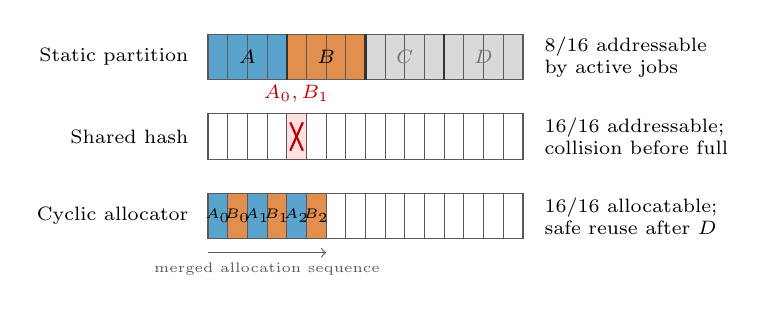
\begin{tikzpicture}[x=0.25cm,y=0.72cm,font=\scriptsize]
% All three rows contain the same sixteen physical slots.  Filled cells in
% the bottom two rows illustrate allocation, not instantaneous occupancy.
\node[anchor=east] at (-0.5,3.4) {Static partition};
\foreach \i in {0,...,3}  {\fill[ArborBlue!65]   (\i,3.0) rectangle +(1,0.8);}
\foreach \i in {4,...,7}  {\fill[ArborOrange!70] (\i,3.0) rectangle +(1,0.8);}
\foreach \i in {8,...,15} {\fill[ArborLightGray] (\i,3.0) rectangle +(1,0.8);}
\foreach \i in {0,...,16} {\draw[black!65,line width=0.35pt] (\i,3.0) -- (\i,3.8);}
\draw[black!65,line width=0.45pt] (0,3.0) rectangle (16,3.8);
\foreach \i in {4,8,12} {\draw[black!80,line width=0.8pt] (\i,3.0) -- (\i,3.8);}
\node at (2,3.4) {$A$};
\node at (6,3.4) {$B$};
\node[text=black!55] at (10,3.4) {$C$};
\node[text=black!55] at (14,3.4) {$D$};
\node[anchor=west,align=left] at (16.6,3.4) {8/16 addressable\\by active jobs};

\node[anchor=east] at (-0.5,2.0) {Shared hash};
\foreach \i in {0,...,15} {\fill[white] (\i,1.6) rectangle +(1,0.8);}
\fill[red!12] (4,1.6) rectangle +(1,0.8);
\foreach \i in {0,...,16} {\draw[black!65,line width=0.35pt] (\i,1.6) -- (\i,2.4);}
\draw[black!65,line width=0.45pt] (0,1.6) rectangle (16,2.4);
\draw[red!75!black,line width=0.8pt] (4.18,1.75) -- (4.82,2.25);
\draw[red!75!black,line width=0.8pt] (4.82,1.75) -- (4.18,2.25);
\node[anchor=south,text=red!75!black] at (4.5,2.43) {$A_0,B_1$};
\node[anchor=west,align=left] at (16.6,2.0) {16/16 addressable;\\collision before full};

\node[anchor=east] at (-0.5,0.6) {Cyclic allocator};
\foreach \i in {0,...,15} {\fill[white] (\i,0.2) rectangle +(1,0.8);}
\foreach \i in {0,2,4} {\fill[ArborBlue!65]   (\i,0.2) rectangle +(1,0.8);}
\foreach \i in {1,3,5} {\fill[ArborOrange!70] (\i,0.2) rectangle +(1,0.8);}
\foreach \i in {0,...,16} {\draw[black!65,line width=0.35pt] (\i,0.2) -- (\i,1.0);}
\draw[black!65,line width=0.45pt] (0,0.2) rectangle (16,1.0);
\node[font=\tiny] at (0.5,0.6) {$A_0$};
\node[font=\tiny] at (1.5,0.6) {$B_0$};
\node[font=\tiny] at (2.5,0.6) {$A_1$};
\node[font=\tiny] at (3.5,0.6) {$B_1$};
\node[font=\tiny] at (4.5,0.6) {$A_2$};
\node[font=\tiny] at (5.5,0.6) {$B_2$};
\draw[->,black!65] (0,-0.05) -- node[below,font=\tiny] {merged allocation sequence} (6,-0.05);
\node[anchor=west,align=left] at (16.6,0.6) {16/16 allocatable;\\safe reuse after $D$};
\end{tikzpicture}

\caption{同一份 16-slot 物理容量在三种分配方式下的状态示意。配置四个
job，仅 $A/B$ 活跃：静态分区把 $C/D$ 的预留（灰色）留在原地；共享哈希
允许活跃任务寻址全池，但两个 offset 仍可能在其它地址空闲时碰撞；共享
循环 allocator 把全部活跃 allocation 合并为一个序列，在安全深度 $D$ 之后
覆盖复用。填色表示地址所有权或示例 allocation，不表示某一时刻的实际
占用率。}
\label{fig:motivation-state-allocation}
\end{figure}

\begin{table}[t]
    \centering
    \caption{典型在网聚合系统的状态所有权、原语覆盖与位置选择。}
    \label{tab:inc-comparison}
    \small
    \setlength{\tabcolsep}{3pt}
    \begin{tabularx}{\linewidth}{@{}p{0.11\linewidth}p{0.13\linewidth}p{0.11\linewidth}p{0.16\linewidth}Xp{0.14\linewidth}@{}}
        \toprule
        系统 & 状态位置 & 所有权范围 & 原语覆盖 & 位置选择 & 不可用时的处理 \\
        \midrule
        SwitchML~\cite{switchml} & 交换机 SRAM & 任务级分区 & 梯度 AllReduce & PSN 分区内循环复用 & 端侧窗口等待/恢复 \\
        NetReduce~\cite{netreduce} & RDMA 路径 FPGA & 路径上下文 & AllReduce & RDMA 报文拦截 & 端点 RoCE 恢复 \\
        SHARP~\cite{sharp} & 硬件 reduction tree & 通信组映射 & Reduce/AllReduce/Barrier & 预配置 tree & 通信库与硬件处理 \\
        EPIC~\cite{epic} & 交换机/加速器 SRAM & 组与连接 context & AllReduce/Reduce/Broadcast & PSN 窗口循环复用 & mode-specific ACK/NAK \\
        ATP~\cite{atp} & 交换机 SRAM & 跨任务共享 & 梯度 AllReduce & job/sequence hash & 参数服务器补全 \\
        AIRP~\cite{airp} & 网络内聚合器 & 控制面共享 & 随底层 INC & 全局资源规划 & 依赖底层 INC \\
        \bottomrule
    \end{tabularx}
\end{table}

\Cref{fig:motivation-state-allocation} 中的比例表示\emph{活跃任务可寻址的
状态}，而非当前非空 slot 的比例。任务级分区只让活跃任务使用自己的份额；
数据面哈希可以寻址全池，却不保证未满时没有碰撞；控制面规划有全局视图，
但受分配粒度和更新周期限制。\Cref{tab:inc-comparison} 把这些机制映射到
代表性系统。

\parab{共享哈希仍会留下不可用容量.}
\Cref{fig:motivation-hash-conflicts} 固定 $N=4,J=4$、端侧控制规则和链路
配置，仅改变 ATP 的物理聚合器数 $A$。哈希冲突率总体从 $A=8$ 时的
68.31\% 降至 $A=512$ 时的 1.08\%；在 $A=1024$ 的
3,440,448 次 aggregation attempt 中未观测到哈希冲突。有限测量中的零次
冲突并非普适保证：在 $8\le A\le960$ 的其余已测配置中，静态 job/sequence
映射仍会发生冲突，并把相应 packet 转入回退路径。

\begin{figure}[t]
\centering
\begin{tikzpicture}
\begin{axis}[
  arbor axis,
  width=0.96\linewidth,height=0.53\linewidth,
  xmin=8,xmax=1024,ymin=0,ymax=70,
  xtick={8,128,256,512,768,1024},
  ytick={0,10,20,30,40,50,60,70},
  xlabel={物理聚合器数 $A$},
  ylabel={哈希冲突率（\%）},
]
\addplot[ArborOrange,thick,mark=*,mark size=1.0pt]
  table[col sep=comma,x=physicalAggregators,y=atpHashCollisionPct]
    {plots/data/pgf/motivation-atp-hash-collisions.csv};
\end{axis}
\end{tikzpicture}

\caption{ATP 的物理聚合器数与哈希冲突率。测试床固定为 $N=4,J=4$、
每 job 每 rank 64-MiB AllReduce、8-KiB payload、端侧控制规则和链路配置；
曲线扫描全部 51 组物理聚合器配置 $A$。哈希冲突率为 FPGA 记录的 collision
数占全部 root aggregation attempts 的比例，每点汇总五个 fresh process。
$A=1024$ 的 3,440,448 次 attempt 中未观测到 collision。横纵轴均为线性
坐标。}
\label{fig:motivation-hash-conflicts}
\end{figure}

安全定容与地址覆盖因此是两个不同的问题：对共享池，全部 job 的 allocation
合并为一个推进序列并决定安全深度；达到该深度后，位置选择机制才决定已配置
地址是否都能成为活跃任务的可用容量。\Cref{sssec:slot-bound} 给出循环映射
的精确条件和部署界，\cref{ssec:eval-state} 再量化三种分配方式达到同一
性能目标所需的状态。

\section{现有组内协调依赖特定传输边界}
\label{ssec:group-consistency}

点对点 ACK、ECN、窗口和路径状态天然对应一个 sender--receiver 关系或本地
传输段，而同一 offset 的聚合完成取决于整个 fan-in。已有 INC 系统并非
忽略慢分支，而是各自在点对点连接之上建立了组内协调边界。
SwitchML~\cite{switchml} 把任务的 aggregation pool 同时用作发送窗口：
worker 收到聚合结果后才复用对应 slot，慢分支最终通过 pool 的自时钟限制
全组推进。ATP~\cite{atp} 在上行聚合时合并 CE，参数服务器再通过
parameter ACK 把共同信号返回各 worker；多播之后的单条返回分支仍可再次
标记 CE，但该信号只作用于相应 worker，不会在同一轮重新合并为组信号。

EPIC~\cite{epic} 把协调边界进一步移入交换机传输端点：Mode-I 在交换机
终结连接并逐跳流控，Mode-III 维护 pipe、ACK 进度和有效 PSN 范围，其
rate-sync 选项还可由首跳交换机为超前 rank 主动生成 CNP。维持这些边界
本身就有数据面代价：SwitchML 的 pool 同时充当发送窗口，窗口深度与
SRAM 分区互相牵制；ATP 需要参数服务器及其链路承接组信号；EPIC 则在
交换机中保存连接、ACK 进度和有效 PSN 范围等聚合状态之外的传输状态。
这份代价还随原语分化——EPIC 的 AllReduce、Broadcast 和 Reduce 分别
需要 ACK 改写反射、逐级 ACK 聚合和沿树 ACK 广播，非对称原语还要对齐
各 rank 的序号漂移；每支持一种原语，交换机传输端点上就多一份数据面
处理逻辑与存储（\cref{tab:inc-comparison} 的原语覆盖列）。因此，这些
机制都能约束分支偏斜，代价是把组内推进分别绑定到 aggregation pool、
参数服务器或交换机侧传输状态，并让原语覆盖成为数据面实现的函数。下面的
实验量化这些边界需要吸收的底层代价，而不是把它们简化为``对慢分支没有
响应''。

\parab{一条慢分支仍会扩大状态的保护区间.}
无论协调边界位于 pool、参数服务器还是交换机传输端点，聚合器都必须等同一
offset 的全部输入到齐：若一条分支与其它流共享瓶颈，快分支的输入先到也
不能单独提交，部分聚合值要一直保留到慢分支补齐。协调机制允许的到达偏斜
因而直接决定状态持有时间，也决定循环 allocator 在安全复用前必须跨越的
slot 窗口。

\begin{figure}[t]
\centering
\begin{minipage}[b]{0.46\linewidth}
\centering
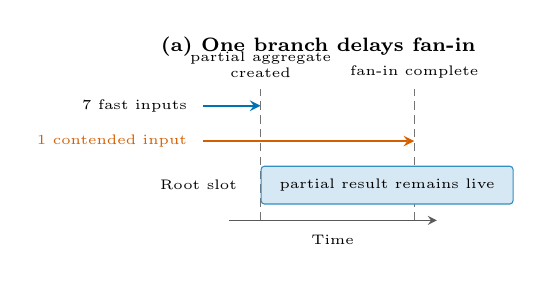
\begin{tikzpicture}[
  x=0.61cm,y=0.56cm,font=\scriptsize,
  arrival/.style={-stealth,line width=0.7pt},
  event/.style={black!55,densely dashed,line width=0.45pt},
  state/.style={draw=ArborBlue!80,fill=ArborBlue!16,rounded corners=1.2pt,
    minimum height=0.48cm,align=center,font=\tiny},
]
\node[font=\bfseries\scriptsize,anchor=south] at (3.25,4.05)
  {(a) One branch delays fan-in};

\node[anchor=east,font=\tiny] at (0.72,3.15) {7 fast inputs};
\draw[arrival,ArborBlue] (0.86,3.15) -- (2.05,3.15);
\node[anchor=east,font=\tiny,text=ArborOrange] at (0.72,2.35)
  {1 contended input};
\draw[arrival,ArborOrange] (0.86,2.35) -- (5.25,2.35);

\draw[event] (2.05,0.55) -- (2.05,3.53);
\draw[event] (5.25,0.55) -- (5.25,3.53);
\node[anchor=south,align=center,font=\tiny] at (2.05,3.56)
  {partial aggregate\\created};
\node[anchor=south,align=center,font=\tiny] at (5.25,3.56)
  {fan-in complete};

\node[anchor=east,font=\tiny] at (1.76,1.35) {Root slot};
\node[state,anchor=west,minimum width=3.20cm] at (2.05,1.35)
  {partial result remains live};
\draw[-stealth,black!65,line width=0.45pt] (1.40,0.55) -- (5.72,0.55);
\node[anchor=north,font=\tiny] at (3.55,0.43) {Time};
\end{tikzpicture}
\end{minipage}\hfill
\begin{minipage}[b]{0.51\linewidth}
\centering
\begin{tikzpicture}
\begin{axis}[
  arbor axis,arbor panel,
  width=\linewidth,height=0.50\columnwidth,
  title={(b) Measured state expansion},
  xmin=0.8,xmax=4.6,
  ymin=-0.45,ymax=1.45,
  xtick={1,2,3,4},
  xticklabels={1x,2x,3x,4x},
  ytick={0,1},
  yticklabels={{State holding p99\\$31.8\!\rightarrow\!127.2~\mu$s},
    {Safe reuse depth\\$89\!\rightarrow\!229$ slots}},
  y dir=reverse,
  xmajorgrids=true,
  ymajorgrids=false,
  yticklabel style={font=\scriptsize,align=right},
  xlabel={Increase over no contention},
]
\addplot[black!70,thin,densely dotted,mark=none,forget plot]
  coordinates {(1,-0.45) (1,1.45)};
\addplot[
  ArborGray,only marks,mark=square*,mark size=2.0pt,forget plot,
]
  table[col sep=comma,x expr=1,y=x]
    {plots/data/pgf/motivation-branch-skew.csv};
\addplot[
  ArborBlue,only marks,mark=*,mark size=2.4pt,
  nodes near coords,
  point meta=explicit symbolic,
  every node near coord/.append style={font=\scriptsize,anchor=west,xshift=2pt},
  error bars/.cd,x dir=both,x explicit,
]
  table[col sep=comma,x=relative,y=x,x error=relativeCi,meta=label]
    {plots/data/pgf/motivation-branch-skew.csv};
\end{axis}
\end{tikzpicture}
\end{minipage}

\caption{单条受竞争分支扩大聚合状态的保护区间。(a) 同一 offset 的七个
输入先到，root slot 持续保存部分结果，直到受竞争分支的最后一个输入到达。
(b) root 状态的 p99 持有时间由 31.8 增至 127.2~\textmu s，安全循环复用
深度由 89 增至 229 slots，分别为无背景流时的 4.0 和 2.6 倍。点为三条配对
物理分支的均值，误差线为 Student-t 95\% CI。}
\label{fig:motivation-branch-skew}
\end{figure}

为隔离这一效应，\cref{fig:motivation-branch-skew} 把一个 8-rank
AllReduce 固定到同一棵树上，只加入一条持续点对点流，与其中一条 200-Gbps
上行链路竞争。root 状态的 p99 持有时间从 31.83 增至 127.24~\textmu s，
完整 slot 事件轨迹给出的安全循环复用深度从 89 增至 229；树、聚合位置和
其它链路均保持不变，8192-slot 配置不构成瓶颈，全部运行也没有丢包、PFC、
\texttt{AGG\_MISS}、overwrite 或 repair。增长因此只来自单条分支拖延整组
完成，与聚合状态不足或恢复流量无关。这个对照实验固定发放行为，没有复现
上述系统完整的自时钟、参数服务器或逐跳流控；它量化的是这些机制共同需要
约束的状态生命周期，其中的 p99 也只是有限运行中的观测值，不是定容所需的
硬上界。\Cref{ssec:eval-cc} 在相同的固定单树、禁止换路条件下，进一步
比较不同反馈范围如何控制发送。

\parab{候选树之间的剩余容量不一致.}
ECMP~\cite{ecmp} 在 flow 粒度固定路径；Themis~\cite{themis} 用确定性的
PSN--path 映射喷洒 packet，常规分配同样由报文标识决定，不响应持续的路径
不对称。CONGA~\cite{conga} 和 LetFlow~\cite{letflow} 等自适应方案按网络
反馈在 flowlet 或 packet 粒度迁移后续流量，但一次决策只移动一个单播
packet 或 flowlet。聚合树的剩余容量不同时，固定映射会把一部分 offset 留
在慢树上；自适应单播能迁移后续流量，却决定不了同一 offset 的整组输入该
使用哪棵聚合树。

\parab{在网 fan-in 改变选路的决策单位与一致性义务.}
单播多路径中，一次选路决策的错误代价是乱序或次优路径
（\cref{ssec:p2p-ccl}）。在网 fan-in 下，为一个 packet offset 选择聚合树
是一次整组决策：它同时确定整组输入经过的链路和逐级聚合位置。这一决定必须
传达给全部 requester，而不同分支上的控制信息可能以不同顺序到达。若各
requester 仅按本地连接状态把一次选树决定绑定到``下一个未发送 packet''，
同一决定就可能对应不同 offset，使一轮 fan-in 合并不同数据的输入。一棵
固定树天然避免该错误，却无法利用其它树的动态剩余容量；静态条带化也只能
在预定比例内保持一致。本文把自适应方案必须维持的关系称为\emph{聚合上下文
一致性}：同一 packet offset 的全部输入必须导出同一棵树和同一份逐级聚合
上下文。

\section{上下文与反馈要求及多播-聚合流}
\label{ssec:inc-limits}

传输层因此需要满足两项要求。\emph{聚合上下文一致性}要求同一 offset 的
输入进入同一棵树，并在共享的每一级使用一致的聚合位置；\emph{整组进度
可见性}要求发送控制、后续选树和恢复依据覆盖最慢分支的完成边界或组级拥塞
信号。多租户状态管理还需独立保证上下文在复用前已经安全结束，动态选树才
不必把``是否还有空闲 slot''当作又一个在线决策变量。

本文把同时描述一对多发送与多对一聚合的传输关系称为\emph{多播-聚合流}。
它固定一个 responder 和 requester group，并以 packet offset 作为路径、
聚合上下文、组内推进和恢复的共同语义边界；\cref{chap:design} 给出具体
实现。

\chapter{设计}
\label{chap:design}

\sysname 将多播-聚合流实现为 channel，并以组播 credit 逐 packet offset
推进。Credit Context 绑定 offset 与 subchannel，credit 副本沿下行路径取得
逐级聚合位置；requester 带回这些位置后，request 在上行路径完成聚合。
responder 再以完成事件选择 subchannel、约束后续 credit，并在异常时启动
整组 repair。\Cref{tab:design-sync} 汇总这些规则如何满足
\cref{ssec:inc-limits} 的上下文一致性与整组进度要求。

\begin{table}[t]
    \centering
    \caption{\sysname 用同一组协议字段建立聚合上下文一致性并暴露整组进度。}
    \label{tab:design-sync}
    \small
    \setlength{\tabcolsep}{3pt}
    \begin{tabularx}{\linewidth}{p{0.18\linewidth}YY}
        \toprule
        机制 & 上下文绑定 & 整组进度 \\
        \midrule
        多播-聚合流 &
        定义路径、聚合位置与恢复的共同 packet-offset 边界 &
        把 responder 与 requester group 的 request/response 关系作为一个传输对象 \\
        组播 credit &
        显式绑定 offset、subchannel 与逐级 slot &
        requester group 消费同一份 credit，并继承同一 Credit Context \\
        聚合器位置反馈 &
        response 下行分配 slot，request 上行带回并通过 owner 校验 &
        同一 offset 的所有输入在其共享的每一级命中同一聚合位置 \\
        拥塞控制 &
        responder 以 $r_s$ 和 $W_s$ 两道门约束后续 credit，repair 使用独立预算 &
        fan-in 完成时间反映最慢分支，一份闭环完成时延样本约束整组速率 \\
        可靠性 &
        owner mismatch 生成失配通知，repair request 走旁路，二者都不产生正常完成样本 &
        responder 组播 repair trigger，并用 requester 位图完成整组去重 \\
        \bottomrule
    \end{tabularx}
\end{table}

\section{总体设计}
\label{ssec:design-overview}

运行时把一次原语调用映射为一个或多个 channel message。每个 message 覆盖
一段连续数据，并进一步切成固定大小的 packet。以 \texttt{AllReduce} 为例，
数据按 rank 切片，每个 rank 作为一个切片的 responder，其它 rank 为该切片
提供同一 packet offset 上的输入；其余原语的映射见
\cref{ssec:channel-subchannel}。

\begin{figure*}[t]
\centering
% 设计总览：多播-聚合流与组播 credit（fig:design-overview）
% (a) 一份 normal credit 的组播闭环；(b) 一个 channel 的多棵 subchannel 树
\begin{minipage}[b]{0.56\linewidth}
\centering
\begin{tikzpicture}[x=1cm,y=1cm,
  box/.style={draw,rounded corners=1.5pt,minimum height=0.5cm,
    inner sep=3pt,font=\scriptsize},
  acc/.style={box,fill=ArborLightGray!60},
  ep/.style={box,fill=ArborBlue!12},
  credit/.style={-stealth,ArborBlue,semithick,dashed},
  up/.style={-stealth,ArborOrange,semithick},
  lab/.style={font=\tiny,inner sep=1pt}]
  \node[ep]  (R)  at ( 0.0,4.55) {responder};
  \node[acc] (SP) at ( 0.0,3.15) {加速器};
  \node[acc] (L1) at (-1.9,1.75) {加速器};
  \node[acc] (L2) at ( 1.9,1.75) {加速器};
  \node[ep]  (q1) at (-2.7,0.35) {$q_1$};
  \node[ep]  (q2) at (-1.1,0.35) {$q_2$};
  \node[ep]  (q3) at ( 1.9,0.35) {$q_3$};
  \node[lab,anchor=west] at ( 0.62,3.38) {slot 7};
  \node[lab,anchor=east] at (-2.52,1.98) {slot 3};
  \node[lab,anchor=west] at ( 2.52,1.98) {slot 5};
  % 下行：credit 组播副本，逐级推进 allocator 并压栈
  \draw[credit] (R)  to[bend right=18]
    node[lab,left=2pt]{credit $(k,s_1)$} (SP);
  \draw[credit] (SP) to[bend right=18] (L1);
  \draw[credit] (SP) to[bend right=18] (L2);
  \draw[credit] (L1) to[bend right=18]
    node[lab,left=2pt]{栈 $[7,3]$} (q1);
  \draw[credit] (L1) to[bend right=18] (q2);
  \draw[credit] (L2) to[bend right=18]
    node[lab,right=2pt]{栈 $[7,5]$} (q3);
  % 上行：request 按栈逐级聚合并累计贡献数
  \draw[up] (q1) to[bend right=18] (L1);
  \draw[up] (q2) to[bend right=18] (L1);
  \draw[up] (L1) to[bend right=18] node[lab,right=2pt]{$\times2$} (SP);
  \draw[up] (q3) to[bend right=18] (L2);
  \draw[up] (L2) to[bend right=18] node[lab,left=2pt]{$\times1$} (SP);
  \draw[up] (SP) to[bend right=18]
    node[lab,right=2pt]{$\times3$，完成样本} (R);
  % 图例
  \draw[credit] (-3.30,-0.55) -- (-2.85,-0.55);
  \node[lab,anchor=west] at (-2.80,-0.55) {credit 下行：分配 slot、压位置栈};
  \draw[up] ( 0.55,-0.55) -- ( 1.00,-0.55);
  \node[lab,anchor=west] at ( 1.05,-0.55) {request 上行：按栈聚合};
\end{tikzpicture}
\par\smallskip{\small (a) 一份 normal credit 的组播闭环}
\end{minipage}\hfill
\begin{minipage}[b]{0.40\linewidth}
\centering
\begin{tikzpicture}[x=1cm,y=1cm,
  box/.style={draw,rounded corners=1.5pt,minimum height=0.5cm,
    inner sep=3pt,font=\scriptsize},
  ep/.style={box,fill=ArborBlue!12},
  sw/.style={box,fill=ArborLightGray!60},
  t1/.style={ArborBlue,semithick},
  t2/.style={ArborOrange,semithick,dashed},
  lab/.style={font=\tiny,inner sep=1pt}]
  \node[sw] (SA) at (-0.9,2.05) {$S_A$};
  \node[sw] (SB) at ( 0.9,2.05) {$S_B$};
  \node[ep] (Rb) at (-2.4,0.40) {R};
  \node[ep] (b1) at (-0.8,0.40) {$q_1$};
  \node[ep] (b2) at ( 0.8,0.40) {$q_2$};
  \node[ep] (b3) at ( 2.4,0.40) {$q_3$};
  \foreach \h in {Rb,b1,b2,b3}{
    \draw[t2] (SB) -- (\h);
  }
  \foreach \h in {Rb,b1,b2,b3}{
    \draw[t1] (SA) -- (\h);
  }
  \node[lab,anchor=east,ArborBlue]   at (-1.38,2.42) {树 $s_1$};
  \node[lab,anchor=west,ArborOrange] at ( 1.38,2.42) {树 $s_2$};
  \node[lab,align=center] at (0,3.00)
    {offset：$k\to s_1$，\ $k{+}1\to s_2$，\ $k{+}2\to s_1$，$\cdots$};
  \node[lab,align=center] at (0,-0.30)
    {每棵树独立维护 $r_s$/$W_s$ gate；gate 关闭的树不取得新 offset};
\end{tikzpicture}
\par\smallskip{\small (b) 一个 channel 的多棵 subchannel 树}
\end{minipage}

\caption{多播-聚合流与组播 credit。(a) responder 为 packet offset $k$
在树 $s_1$ 上组播一份 credit；credit 副本逐级推进 allocator、取得 slot
并压入位置栈，requester 凭 credit 发送 request，上行按栈逐级聚合并累计
贡献数，整组到齐（$\times3$）后 responder 获得闭环完成样本。(b) 一个
channel 预装多棵 subchannel 树，responder 按各树的 gate 分配后续 offset；
同一 offset 的全部输入使用同一棵树。}
\label{fig:design-overview}
\end{figure*}

\sysname 把 credit 附在 response 上组播下发：带 credit 的 response 授权
一个 offset 和 subchannel，下行副本沿各自分支取得位置栈。requester 只有
消费该 credit 后才发送对应 request，并带回本分支的位置与逐级 fan-in。
上行聚合结果返回 responder 后，response 可以同时交付结果并授权新的
offset。注册闭环负责 message readiness，数据闭环负责 packet 许可与完成
（\cref{fig:design-overview}(a)）。

\parab{注册闭环.}
responder 只有在全组安装一条消息的本地状态后，才能为该消息发放 normal
credit。requester 提交消息后，在各 subchannel 上周期发送轻量
\texttt{REGISTER}；responder 为每个 message/subchannel 收集 requester
readiness，并在本地消息也已提交后组播 \texttt{REGISTER\_ACK}。周期发送
容忍控制包丢失，确认后 requester 停止对应信标。注册只确认 readiness，
不授予 request 发送。\sysname 只让正常路径的包经过加速器，其余包由网络
直接转发；拥塞控制也不采集注册阶段的样本。后续消息可以在当前消息传输期间
异步注册，因此注册闭环不要求 channel 在消息边界停顿。

\parab{Credit 驱动的数据闭环.}
responder 按每个 subchannel 的速率门和窗口门发放 credit。Credit 通过
response packet 组播给 requester group，使整组获得同一 offset 和
subchannel 的后续许可；response 副本沿各自分支携带聚合器位置，同一聚合
子树内的对应位置一致。readiness 完成后的数据 request 必须凭 credit 发送；
同一个 response 可以返回一个 packet 的数据或完成信息，并授权另一个
packet 的 request。负载均衡、拥塞控制与聚合器复用都由该 response/credit
闭环驱动。

\section{Channel 与 Subchannel}
\label{ssec:channel-subchannel}

channel 是多播-聚合流的协议表示：一个 channel 固定 responder 和
requester group，并依次承载多个 message。subchannel 是该 channel 在具体
拓扑上的一棵聚合树；每个 channel 独立定义自己的 subchannel 集合，不同
集合可以共享物理链路（\cref{fig:design-overview}(b)）。不同 packet
offset 可以选择不同 subchannel；同一 offset 的全部输入必须使用 credit
指定的同一棵树。

\Cref{tab:collective-mapping} 通过 channel 集合和用户 payload 方向表达
六种原语。``全部 rank''表示每个 rank 对应的 channel 都承载一个数据切片；
``root''只使用 root 对应的 channel。表中的有/无仅描述应用数据方向：
\texttt{Reduce} 和 \texttt{ReduceScatter} 的 response 仍携带 completion
与 credit，\texttt{Barrier} 的两个方向仍使用控制 packet。所有原语复用
相同的 credit、选树、聚合和恢复规则。

\begin{table}[t]
\centering
\caption{\sysname 在同一传输层数据通路上表达六种集合通信原语，差异仅在于
channel 集合的选择与 request/response 中用户 payload 方向的配置。}
\label{tab:collective-mapping}
\begin{tabular}{lccc}
\toprule
原语 & Channel & Request payload & Response payload \\
\midrule
AllReduce & 全部 rank & 有 & 有 \\
Reduce & root & 有 & 无 \\
Broadcast & root & 无 & 有 \\
AllGather & 全部 rank & 无 & 有 \\
ReduceScatter & 全部 rank & 有 & 无 \\
Barrier & 全部 rank & 无 & 无 \\
\bottomrule
\end{tabular}
\end{table}

\parab{Credit Context.}
在一个 channel 中，一份 credit 以 \texttt{(channel\_id, packet\_offset,
subchannel\_id)} 定义一个 \emph{Credit Context}。\texttt{packet\_offset}
标识本轮被授权的 packet，\texttt{subchannel\_id} 指定对应的聚合树。消费
同一份 credit 的 requester 继承同一 Credit Context；responder 按
\texttt{(channel\_id, packet\_offset)} 提交完成结果。

\section{聚合器位置反馈}
\label{ssec:agg-feedback}

聚合树上的每一级加速器维护一个 allocator 和一个共享 slot 池；同一加速器
的所有端口共用该池。Normal credit 沿下行路径经过各级加速器，每一级推进
allocator，将取得的 slot 的 owner 设为该 credit 的 Credit Context，并把
slot 编号压入位置栈。requester 因而只会收到已经取得沿途全部聚合位置的
normal credit。Repair trigger 不分配 slot。

\parab{Request 按位置栈逐级聚合.}
requester 把 credit 返回的位置栈和逐级 fan-in 写入 request。若本级
fan-in 为 1，加速器弹栈直转；否则按栈顶定位 slot，并验证 request 的
Credit Context 与 slot owner。首个需要合并的输入绑定 fan-in、算子和
payload shape；数据面同时检查输入是否属于当前支持的 data-type profile。
后续输入通过相同参数检查后累加贡献数和 payload。单个 requester 输入贡献
1，下层聚合结果贡献其携带的计数。贡献数达到本级 fan-in 后，加速器发出
aggregated packet、弹出本级位置，并由上一级继续处理。\texttt{Broadcast}
和 \texttt{AllGather} 使用同一计数路径合并空 request。

所有聚合参数均随 request 携带，加速器无需预装通信组、rank 或源地址表。
requester 对同一 Credit Context 至多发送一份 normal request；repair
request 直接旁路。因此，slot 保存 owner、聚合元数据、贡献数和累加结果，
但不保存 requester 身份或 per-requester bitmap。成员确认和 repair 去重由
responder 完成。

\parab{Owner 失配终止正常聚合.}
owner 失配表示 credit 许诺的 slot 已被新的 Credit Context 覆盖。加速器
丢弃 payload，并把 packet 改写为 header-only 的 \texttt{AGG\_MISS}；该
通知不再进入后续各级的正常聚合。responder 收到通知后将对应 credit 原子地
切换到 repair mode，并组播 repair trigger（\cref{ssec:reliability}）。
通知丢失时，原 credit 的超时器触发相同恢复过程。该规则同样处理单个输入和
下层 aggregated packet，不会把部分结果带入后续聚合级。

\parab{覆盖复用无需端到端释放.}
循环 allocator 通过覆盖复用 slot：normal credit 取得 slot 后，加速器
原子地安装新的 Credit Context owner 并重置逻辑聚合状态。旧 owner 的迟到
request 因 owner mismatch 产生 \texttt{AGG\_MISS}，responder 随后切入
repair。该规则把 slot 生命周期限制在本级：安全时刻由本级结果读出或
responder 的 repair cutover 确定。allocator 不等待端点或控制面发出显式
释放消息，也不维护分布式 aggregation-slot free list。加速器仅在把本级
结果复制到独立的完成缓冲区期间短暂阻止覆盖对应 slot；由此，slot 回收从
端到端协议状态变为加速器内部的局部覆盖操作。每一级独立维护循环指针和
owner；插入新的聚合层级只扩展 credit 的位置栈，不增加端点对该级 slot 的
分配或释放状态。\Cref{sssec:slot-bound} 给出不提前覆盖正常 Context 的
循环深度；深度不足时，被提前覆盖的 Context 转入 repair，旧部分结果仍
不能进入新 Context。

\section{Credit Context 与多路径选择}
\label{ssec:response-credit}
\label{ssec:packet-binding}

\parab{Credit Context 唯一性.}
多个 subchannel 的 response/credit 并行返回时，不同 subchannel 的 credit
在不同 requester 上可能以不同相对顺序到达。若 requester 按本地``下一个
未发送 packet''消费每个到达的 credit，同一份组播 credit 就可能在不同
requester 上绑定到不同 packet offset，使同一轮 fan-in 混入不同 packet 的
输入。\sysname 因此要求一份逻辑 credit 在所有 requester 上导出同一个
Credit Context，把聚合上下文一致性（\cref{ssec:group-consistency}）落实
为可检查的协议不变量。设组播 credit $C$ 逻辑上对应的 \texttt{channel\_id}、
\texttt{credit\_offset} 和 \texttt{subchannel\_id} 分别为 $c(C)$、
$k_c(C)$ 和 $s(C)$；requester $q \in Q$ 用 $C$ 实际发送的 request 继承的
三元组为 $(c_q(C), \mathrm{offset}_q(C), s_q(C))$。本文称如下条件为
\emph{Credit Context 唯一性}：
\begin{equation}
    \forall q \in Q,\quad
    (c_q(C), \mathrm{offset}_q(C), s_q(C))
    =
    (c(C), k_c(C), s(C)).
    \label{eq:credit-context-uniqueness}
\end{equation}

Credit Context 唯一性是组播 credit 的协议不变量。credit 确定 channel、
packet offset 和 subchannel；requester 据此选择 packet 和聚合树，并带回
沿途取得的位置栈（\cref{ssec:agg-feedback}）。未收到该 credit 的
requester 不会为对应 offset 发送 request。缺失输入和 response 由
\cref{ssec:reliability} 的恢复机制处理。

\parab{Payload/Credit offset 绑定.}
一个 response packet 可以返回 packet $p$ 的 payload 或完成信息，并用
credit 授权 packet $k$ 的 request。协议分别使用 \texttt{payload\_offset}
和 \texttt{credit\_offset} 绑定这两项语义；二者可以相同，也可以不同。
\texttt{Broadcast} 和 \texttt{AllGather} 主要使用前者，\texttt{Reduce}
和 \texttt{ReduceScatter} 主要使用后者，\texttt{AllReduce} 同时使用二者。
Credit Context 唯一性约束 credit 授权的 offset，不受 response payload
顺序影响。

\parab{反馈驱动的逐-offset 选树.}
responder 以 packet offset 为单位在多个预装 subchannel 间发放 credit。
每个 subchannel 都有速率门 $r_s$ 和窗口门 $W_s$；只有发放间隔到期且
未完成 credit 数小于 $W_s$ 时，该 subchannel 才能接收新的 packet
offset。responder 在当前允许发放的 subchannel 间分配后续 offset，拥塞或
恢复增多的 subchannel 因速率门收紧或窗口耗尽而获得更少 offset。已经发出
的 Credit Context 始终绑定原 subchannel，不在途换树。

\section{端到端拥塞控制}
\label{ssec:cc}

\parab{端点通过速率门和窗口门控制注入.}
\sysname 不依赖运行时集中式控制器：普通交换机的转发与组播表项在建组前
预装，responder 在本地更新每个 subchannel 的 $r_s$ 和 $W_s$，聚合加速器
不参与拥塞控制决策。requester 只凭 credit 发送，因此 responder 可以用
两道门控制每个 subchannel：速率门要求相邻 credit 的发放间隔不小于
$P/r_s$，窗口门要求未完成 credit 数小于 $W_s$，其中 $P$ 是一份 credit
授权的 packet 字节数，$r_s$ 和下式的 $x_s$ 均以 byte/s 计。令 $T_s$ 为该
subchannel 的稳态闭环完成时延，则 requester 分支上的稳态注入速率满足
\begin{equation}
    x_s \le \min\left\{r_s,\frac{W_sP}{T_s}\right\}.
    \label{eq:cc-two-gates}
\end{equation}
Rate-based、window-based 和 hybrid 控制律分别更新 $r_s$、$W_s$ 或二者。
小数窗口用 $W_s=1$ 加 pacing 表示。显式标记和基于完成时延的算法共用该
credit 发放接口，具体映射见 \cref{app:rate-modules}。

\parab{闭环完成时延覆盖当前最慢分支.}
responder 记录每份 credit 的发出时刻；当返回结果首次证明全组输入已经完成
时，两者之差给出其\emph{闭环完成时延}。该时间覆盖 credit 组播下行、
requester 消费、request 上行和 fan-in 聚合。令 $\mathcal{B}_s$ 表示
subchannel $s$ 上从 responder 经 requester 再返回的分支集合，$d_b$ 表示
分支 $b$ 对本轮完成的时延，则
\begin{equation}
    T_s=\max_{b\in\mathcal{B}_s} d_b.
    \label{eq:completion-delay}
\end{equation}
requester 发送路径停顿和网络排队都可以进入 $d_b$；消息提交偏斜由此前的
注册闭环吸收，不进入 normal credit 样本。只有决定最大值的分支直接改变
本轮完成时间。一份 credit、一次整组完成和一个 $T_s$ 使整组 requester
共享同一速率样本，无需沿途设备维护 per-flow 速率状态。

\parab{最大完成时延过滤非关键分支排队.}
考虑共享链路 $E$ 上增加的闭环排队时间 $q_E$。对一条经过 $E$ 的 channel
$i$，令 $S_i$ 为经过 $E$ 的分支中最大的无队列完成时延，$M_i$ 为其余分支
中的最大值；若所有分支都经过 $E$，定义 $M_i=-\infty$。于是
\begin{equation}
    T_i(q_E)=\max\{M_i,S_i+q_E\},\qquad
    \Delta_i=\max\{0,M_i-S_i\}.
    \label{eq:branch-slack}
\end{equation}
当 $q_E<\Delta_i$ 时，链路 $E$ 尚未决定该 channel 的完成时间，基于完成
时延的模块不会因这部分排队降低整组速率。此时降速不能直接缩短该 channel
的 fan-in 完成时间，反而会减少真正关键分支获得的流量。$q_E$ 达到
$\Delta_i$ 后，经过 $E$ 的分支成为当前最慢分支，后续排队完整进入 $T_i$。
因此，完成时延只让影响 collective 进度的分支直接参与速率调节。

\parab{共享链路上的公平性取决于分支余量.}
多个 channel 共享 $E$ 时，其 $\Delta_i$ 可以不同。若 $E$ 已是 channel
$j$ 的关键分支，却仍落在 channel $i$ 的非关键分支上，$j$ 会先观察到排队
并降速，$i$ 在 $q_E<\Delta_i$ 期间保持原速率。当 $i$ 已受其它分支限制且
不超过 $E$ 的剩余容量时，该行为避免无效退让；否则，非对称路径、
responder 放置和共享链路竞争会产生放置相关的公平性偏置。若所有竞争
channel 都以 $E$ 为关键分支，行为退化为所选控制律在共享瓶颈上的行为；
ECN 则可独立暴露任意分支上的队列。\Cref{ssec:eval-cc} 量化该吞吐与
公平性权衡。

\parab{参考状态与样本筛选.}
responder 在发放 credit 时保存所选控制律所需的参考状态，使返回样本按
发出时状态解释，避免用已经更新过的当前状态重复响应同一次拥塞。一份
normal credit 首次完成时产生一个样本；\texttt{AGG\_MISS}、repair、重放和
已经提交后的迟到输入不产生新样本，修复流量由 \cref{ssec:reliability} 的
独立预算限速。显式标记、rate-based、window-based 与 hybrid 模块所需信号
及其在该接口上的对应关系见\cref{app:rate-modules}。

\parab{显式 ECN 只需传播整组标记.}
基于 completion delay 的端侧算法只使用 responder 本地状态，不要求数据面
增加拥塞控制逻辑。可选 ECN 算法让 requester 把下行 credit 上的 CE 回显到
下一份 normal request，并在逐级聚合时对各输入的 CE 取 OR。responder 因而
获得覆盖上下行路径和全组分支的单个标记。该传播不引入 per-flow 拥塞状态，
控制律仍只在 responder 执行（\cref{app:rate-modules}）。

\section{可靠性与重传}
\label{ssec:reliability}

\sysname 将正常路径的纯计数与恢复路径的身份去重分开。requester 在正常
路径保证单注入，加速器按贡献数完成聚合；异常发生后，responder 将整个
Credit Context 切换到 repair，并用 requester 位图完成去重和回退聚合。

\parab{Normal request 单注入.}
requester 对每个 Credit Context 至多发出一份 normal request。同一份
credit 在 requester 本地只消费一次；之后对该 packet offset 的重发只由
repair trigger 触发，并携带 repair 标志。repair request 旁路 slot。
Normal request 在上行路径不被复制，因此同一 Credit Context 可以按贡献数
聚合；repair 去重和幂等提交由 responder 位图处理。

\parab{Responder 单点提交与重传.}
responder 为每份 normal credit 保留未完成记录，并采用与 ATP 类似的单次
提交语义~\cite{atp}。正常聚合结果只有在贡献数等于 requester group 规模时
才能提交；提交后缓存的 response 不再被迟到输入改写。responder 是唯一的
超时检测与恢复发起者，避免多个 requester 对同一份组播 credit 独立产生
NACK。超时或 \texttt{AGG\_MISS} 将未完成 credit 原子地切换到 repair
mode；此后迟到的正常聚合结果不能提交，该 Credit Context 只由 repair 路径
完成。

\parab{组播 repair trigger.}
定时器超时或收到交换机的失配通知（\cref{ssec:agg-feedback}）后，
responder 组播一份 repair trigger，携带 \texttt{(channel\_id,
packet\_offset, subchannel\_id)}。该控制消息标识恢复范围，requester 据此
沿原 subchannel 发送旁路正常聚合的 repair request。repair trigger 必须
组播：responder 只能观察最终到达的 aggregated packet、\texttt{AGG\_MISS}
和 repair request，看不到交换机 slot 中已经累加的部分状态，也无法可靠
判断哪一个 requester 的输入缺失。Repair request 不再进入原 slot，而是
直达 responder。因此恢复边界是整个 requester group：所有 requester 重新
提交，responder 再用位图收齐并去重。Repair 流量使用独立保守预算，且不
产生正常完成样本（\cref{ssec:cc}）。

\parab{Response 重放不创建第二份 normal credit.}
Response 重放不会使同一 requester 为一个 Credit Context 发送第二份
normal request：未完成 credit 以 repair trigger 重发；缓存的尾部
response 保留 normal credit 时，requester 按本地消费记录去重。已经提交的
结果直接从缓存 response 重放，不重新执行聚合。重试耗尽后，该 collective
失败，且不再复用其未确认的 message identifier。

\parab{END 确认消息完成并回收状态.}
消息末尾若干 packet 的 response 之后不再有新的 credit，其交付无法由后续
credit 的消费隐式确认。全部 credit 完成后，responder 组播 \texttt{END}；
requester 在本地消息完成后回复 \texttt{END\_ACK}。确认缺失时，responder
重放尚未被后续 credit 确认的尾部 response，并重新发送 \texttt{END}。握手
完成前，responder 保留相应 response 和消息状态；握手只延迟消息标识符
复用，不阻止已经注册的后续消息使用新的 packet offset。

\section{共享循环 allocator 的容量}
\label{ssec:bounded-state}
\label{sssec:slot-bound}

每台交换机的全部端口和 job 共用一个带 owner 的 slot 池，每个 normal
Credit Context 都推进同一个循环 allocator。本节要回答的问题可以说得很
直白：池子要配多少个 slot，才能保证 allocator 转一圈回到某个地址时，
上面的旧聚合一定已经结束？答案分两步：先给出一个精确的充要条件，再把
它换算成只依赖端口线速的部署上界。

\parab{循环复用的基本结构.}
设池中有 $A_e$ 个 slot，第 $n$ 次 allocation 使用地址 $n\bmod A_e$。
于是同一个地址恰好每隔 $A_e$ 次 allocation 被复用一次：某个 Context
在第 $n$ 次 allocation 拿到 slot 后，下一个使用同址的正是第 $n+A_e$
次 allocation。``复用是否安全''因此只取决于一个数字——从拿到 slot 到
它可以被安全覆盖，allocator 中间又推进了多少次。只要这个数字不超过
$A_e$，轮回到同址时旧 Context 必然已经结束。下面把``可以被安全覆盖''
和``推进了多少次''说精确。

\parab{复用保护区间.}
覆盖一个 slot 唯一的危险，是旧 Context 之后仍可能在本级提交 normal
结果。两类事件都会永久排除这种可能：本级聚合结果已经读出，或
responder 已完成 repair cutover——此后迟到的 normal 结果不再能提交
（\cref{ssec:reliability}）。对经过交换机 $e$ 的 normal Credit
Context $x$，记 $t_a(e,x)$ 为绑定 slot 的时刻，$t_f(e,x)$ 为上述两类
事件中先发生的时刻；$t_f$ 是 $x$ 的\emph{可安全覆盖时刻}，而非协议中
的显式释放事件。半开区间 $[t_a(e,x),t_f(e,x))$ 称为 $x$ 的\emph{复用
保护区间}，取 $R_e>0$ 为其长度的上界。

\parab{精确最小深度.}
令 $N_e(I)$ 表示事件区间 $I$ 内的 normal advance 数，对保护区间从
$x$ 自身的 allocation（含）计到 $t_f$（不含）。所需深度由最坏的
Context 决定：
\begin{equation}
 D_e=\sup_x N_e([t_a(e,x),t_f(e,x))).
 \label{eq:allocator-exact-depth}
\end{equation}
用一句话读这个定义：$D_e$ 是``任何一个 Context 在自己还不能被覆盖的
期间，整台交换机最多又发生了多少次分配''。计数覆盖全部 normal
advance——fan-in 为 1、弹栈直转因而自身可立即覆盖的 Context 也占一次
分配，同样推进循环指针。$D_e$ 只关于全部 job 合并后的同一条分配序列，
池容量因此不需要按 job 或 rank 数再乘静态因子。同一时刻的 $t_f$ 与 allocation 按先释放、后
分配排序；完整记账约定与实现无法保证该顺序时的处理见
\cref{app:allocator-port-bound}。

\begin{theorem}
\label{thm:allocator-exact}
第 $n$ 次 allocation 使用地址 $n\bmod A_e$ 时，normal path 不发生提前
覆盖当且仅当
\begin{equation}
 A_e\geq D_e .
 \label{eq:allocator-exact-condition}
\end{equation}
\end{theorem}

\noindent\emph{证明.}
充分性：任取 Context $x$，设它由第 $n$ 次 allocation 绑定，则复用
同址的是第 $n+A_e$ 次。由 $A_e\geq D_e$，$x$ 的保护区间内至多有
$A_e$ 次 advance（含 $x$ 自身），即区间内的 allocation 至多编号到
$n+A_e-1$；第 $n+A_e$ 次因此不早于 $t_f$——覆盖发生时 $x$ 已可安全
覆盖。必要性：若 $A_e<D_e$，按 \cref{eq:allocator-exact-depth} 存在
Context $x$，其保护区间内的 advance 数超过 $A_e$，于是第 $n+A_e$ 次
allocation 落在 $t_f$ 之前——同一地址在 $x$ 可安全覆盖前就被覆盖。
\Cref{fig:allocator-timeline} 画出这两种情形。\hfill$\square$

\begin{figure}[t]
\centering
\begin{tikzpicture}[font=\scriptsize]
\draw[->,black!70] (-0.2,0) -- (8.6,0);
\fill[ArborBlue,fill opacity=0.12] (0.6,0) rectangle (5.4,0.72);
\draw[ArborBlue,thick] (0.6,-0.14) -- (0.6,0.72);
\draw[ArborBlue,thick,dashed] (5.4,-0.14) -- (5.4,0.72);
\node[ArborBlue!70!black,anchor=south] at (2.8,0.76)
  {复用保护区间 $[t_a,t_f)$，长度 $\leq R_e$};
\node[anchor=north,align=center] at (0.8,-0.22)
  {$t_a$：第 $n$ 次 allocation\\绑定地址 $n\bmod A_e$};
\node[anchor=north,align=center] at (5.6,-0.22) {$t_f$：可安全覆盖};
\foreach \x in {1.3,2.0,2.7,3.4,4.1} \draw[black!55] (\x,-0.09) -- (\x,0.09);
\draw[black!55] (7.1,-0.09) -- (7.1,0.09);
\node[black!55,anchor=south] at (2.35,0.10) {后续 normal advance};
\draw[ArborOrange,thick,->] (4.8,1.46) -- (4.8,0.12);
\node[ArborOrange!85!black,anchor=south,align=center] at (4.3,1.48)
  {第 $n{+}A_e$ 次（$A_e<D_e$）\\提前覆盖};
\draw[ArborGreen!80!black,thick,->] (7.1,1.46) -- (7.1,0.12);
\node[ArborGreen!55!black,anchor=south,align=center] at (7.3,1.48)
  {第 $n{+}A_e$ 次（$A_e\geq D_e$）\\安全复用};
\end{tikzpicture}
\caption{循环复用的时间线。地址 $n\bmod A_e$ 在第 $n{+}A_e$ 次
allocation 时被再次使用：保护区间内的 advance 数不超过 $A_e$（即
$A_e\geq D_e$）时，同址复用必然落在可安全覆盖时刻 $t_f$ 之后；否则第
$n{+}A_e$ 次分配落入区间内，构成提前覆盖。}
\label{fig:allocator-timeline}
\end{figure}

容量不足不改变结果正确性。新 allocation 原子地安装新的 owner 并重置
逻辑聚合状态；覆盖后到达的旧 request 无法通过 owner 检查，并被改写为
\texttt{AGG\_MISS}。若不再有旧 request 到达，responder timeout 仍会
切入 repair。Normal request 单注入又阻止旧 Context 开始第二轮聚合。
欠配因而增加 repair，但不会把旧部分结果提交给新的 Context。

\parab{端口速率把 $D_e$ 换算为部署深度.}
$D_e$ 是协议量，部署者需要能直接从链路参数算出的上界。物理直觉是：
每一次 advance 最终都对应一份至少 $P$ bytes 的 payload packet 经过
某个端口，而端口串行化限制了任何时间窗内能通过的这类包数——一个
100-Gbps 端口发送一个 8-KiB 包约需 0.66~\textmu s，长度 $R_e$ 的窗口
内它至多承载约 $R_e/(0.66~\mu\mathrm{s})$ 次由它见证的推进。形式化地，考虑
每个 advance 都对应一个正常完成的 fixed-$P$ data context；若每个
context 都能与 allocation 后 $R_e$ 内一份至少携带 $P$ bytes 的
payload packet 一一对应，令 $\mathcal P_e$ 为这些 packet 实际经过的
有向端口集合，$C_p$ 为端口 $p$ 的线速，则
\begin{equation}
 D_e\leq
 \sum_{p\in\mathcal P_e}
 \left\lceil\frac{2C_pR_e}{8P}\right\rceil .
 \label{eq:allocator-directed-port}
\end{equation}
若推进 allocator 的 packet 本身就携带至少 $P$ bytes，配对区间从
$2R_e$ 收紧为 $R_e$：
\begin{equation}
 D_e\leq
 \sum_{p\in\mathcal P_e}
 \left\lceil\frac{C_pR_e}{8P}\right\rceil .
 \label{eq:allocator-payload-carrier-bound}
\end{equation}
两条界均按实际推进同一个共享 allocator 的端口求和。payload 配对与
两倍区间的证明，以及面向提供 advance 到达包络保证的实现、不依赖
payload 配对的另一条充分条件，见 \cref{app:allocator-port-bound}。

在 payload 一一配对前提仍成立时，若部署通过 admission、shaping 和
normal-to-repair deadline 保证保护时间不超过 $R_{\max}$，就可以在
上述容量式中直接使用 $R_{\max}$。沿用上面的直觉：100-Gbps 端口、
$P=8192$ bytes、$R_{\max}=100$~\textmu s 时，
\cref{eq:allocator-payload-carrier-bound} 给出 153 个 slot，即约
1.20~MiB payload memory，另加 metadata。部署使用契约保证的
$R_{\max}$，而非运行 trace 中观察到的最大值。

由循环复用的基本结构，任意连续 $A_e$ 次 allocation 恰好访问每个地址
一次；$A_e\geq D_e$ 时，全部已配置 slot 都是无冲突容量，不受哈希冲突
或 per-job 分区碎片影响。\Cref{ssec:eval-state} 在共用端口和端口分散
两种放置中核对实测 $D_e$ 与 \cref{eq:allocator-payload-carrier-bound}。

\chapter{实现}
\label{chap:implementation}

我们基于 DPDK 实现 \sysname 主机运行时，并为 Alveo V80 实现四端口聚合
RTL kernel。物理原型通过 Tofino 连接四个 100-GbE endpoint 端口和四个
V80 accelerator 端口；交换机只执行 unicast/multicast 转发。V80 kernel
暴露四组 packet AXI4-Stream 接口，DCMAC/GTM shell 负责物理网口、FEC、
GT reset 和时钟转换。六种集合通信原语共用同一 channel 数据路径，原语只
决定 channel 集合和 payload 方向。

\section{原型结构}
\label{sec:impl-structure}

\parab{Channel 单写与 shared poller.}
主机运行时由 EAL lcore poller 构成。每条 physical channel 拥有一对 DPDK
队列及独立的 credit、packet-offset 和 message 状态；配置把每条活跃 channel
恰好分配给一个 poller，一个 poller 可以轮询多条 channel。subchannel 使用
不同 UDP 端口，NIC flow steering 将其导入所属 poller 的 RX 队列，poller
再按报头分派到 channel。该映射保持 channel 状态单写，多条 channel 合并轮询
时不引入跨核锁。当前原型为每个本地运行时实例分配独占的 DPDK device 或 VF；
不同通信组仍共享网络中的 allocator。

\parab{异步 message 发布.}
一次 primitive 调用产生若干 channel message，每个 message 再切成
8192-byte packet。异步接口先在固定表中建立全部 message 并预留 packet
offset，随后用 256-bit 原子位图一次性发布；准备失败的 collective 不进入
数据面。调用在发布后立即返回，worker 根据位图事件启动 per-message 注册。
该路径只串行化同一 communicator 的提交，已发布 message 可以并行推进。

\parab{报头与路径编码.}
多级 profile 使用 20-byte header；物理 testbed 的单级 V3 profile 是前
16 bytes 的严格截断，省略后两级位置字段。两种 profile 的前 16 bytes 具有
相同字段和偏移，分别携带 payload offset 和 credit offset，并用独立
valid bit 区分返回数据与发送许可。24-bit packet offset 在 channel 内连续
编号；UDP port 编码 subchannel，因此 slot owner 可以表示为
\texttt{(UDP port, packet offset)}。Normal credit 最多携带三级位置栈，
2-bit \texttt{agg\_depth} 给出栈深，request 用三个对齐字节携带逐级
fan-in。控制包用 message 起始 offset 作为标识符复用 epoch。Normal
credit 只有在取得沿途全部位置后才交付 requester；\texttt{AGG\_MISS}
清除 payload 和位置栈。

\parab{NUMA 局部性与并行扩展.}
$R_{\rm rep}$ 个 replica 为一个 logical channel 建立相互独立的 physical
channel；poller 数量则决定这些 channel 使用多少主机核。两者相互独立：多条
channel 可以共享一个 poller，增加 poller 也不改变 channel、subchannel 或
credit 的协议语义。每个 channel 的 NIC 队列、mbuf pool 和状态环按其 poller
放置到本地 NUMA 节点；跨 socket 绑定需要显式启用。用户 buffer 的放置仍由
上层应用决定。\Cref{sssec:eval-endpoint-cpu} 分别扫描 replica 与 poller，
并报告达到目标链路速率所需的最小协议核数。

\parab{零拷贝 request 与分段接收.}
运行时把用户输入 buffer 注册给 NIC，并用 DPDK external buffer 将
payload 切片直接挂到 header mbuf 后。首发和 repair request 共用该
payload；repair 只重建 header。接收路径使用 NIC RX buffer split 分离
header 与 payload。requester 解析 header 后，将 response payload 一次
拷贝到用户输出 buffer。

\parab{可选的 I/OAT 交付路径.}
写回用户输出 buffer 的这次搬运有两条已注册路径：poller 直接执行 CPU
拷贝，或交给同 NUMA 节点的 I/OAT DMA 引擎、poller 只提交描述符并回收
完成。两条路径不改变协议语义，也不增加 poller；按 primitive 和消息
大小的路径选择在正式测量前冻结
（\cref{app:physical-implementation-audit}）。

\parab{Requester 无定时器、无重传状态.}
requester 维护一个 credit 队列和一个按 packet offset 取模的去重环，环深
为 $2\times\texttt{MAX\_WINDOW\_SIZE}$。Normal offset 单调推进，稳态
message 查找只检查当前与下一条 message；repair 才扫描完整表。Response
payload 按 \texttt{payload\_offset} 去重写回，credit 则连同 subchannel、
位置栈和 CE 状态入队。发送循环逐项构造 request，并带回位置栈、fan-in
和 CE。

每个未确认 message 的 \texttt{REGISTER} 在 channel 级预算内轮转发送；
\texttt{REGISTER\_ACK} 或首份 credit 停止其信标。注册门阻止 responder 在
全组 message 状态发布前发放 normal credit。requester 不维护数据重传
定时器；收到 repair trigger 后重发 repair request，由 responder 位图
去重（\cref{ssec:reliability}）。

\parab{未完成 credit 表与聚合 slot 合一.}
responder 将未完成 credit 表与主机聚合状态合并为一个按 packet offset
取模的状态环，深度同样为 $2\times\texttt{MAX\_WINDOW\_SIZE}$。entry 在
credit 发放时创建，并保存 requester 位图、master response、subchannel、
提交/repair 状态、重试次数、时间戳和拥塞控制参考状态。端侧拥塞控制模块
取得首个有效样本前，启动窗 $W_0$ 限制总在途 credit。环绕遇到仍承担重放
责任的 entry 时，responder 暂停发放，不会覆盖未确认结果。

交换机聚合结果和 repair 路径的主机聚合结果写入同一份 master response。
已提交结果用 mbuf clone 重放，不重新执行聚合。worker 每轮按固定步长扫描
状态环；超时触发组播 repair，独立 token bucket 限制 repair 流量。Master
response 保留到绑定它的后续 credit 完成；没有后续 credit 的尾部结果保留
到 \texttt{END\_ACK}。

\parab{消息结束与标识符复用.}
\texttt{END}、\texttt{END\_ACK} 和注册包都携带 message 起始 offset 作为
复用 epoch。requester 为最近完成的 epoch 保留 tombstone，因此 message
ID 复用后仍能回答迟到的 \texttt{END}。responder 在收齐 \texttt{END\_ACK}
前保留尾部 response；状态环绕回这些 entry 时暂停新 credit。

\section{聚合加速器：协议把数据面化简为计数与累加}
\label{sec:impl-accel}

端点维护单注入、成员和恢复状态；加速器只保存聚合中的 Credit Context。
加速器旁接商用交换机，不安装通信组、rank、IP/MAC 或转发表。

\parab{Request 自含聚合参数.}
request 用 credit 返回的位置栈直接索引本级 slot，并用
\texttt{(UDP port, packet offset)} 验证 owner。fan-in、算子和数据类型均
随 request 到达。RTL 解析固定偏移字段、推进位置栈，并完成 owner 比较、
计数和累加。当前 data-type profile 支持 FP32 的 SUM/MAX/MIN；其它数值
格式是 profile 扩展，不改变协议字段或恢复规则。聚合结果携带贡献计数，
responder 提交前验证其等于 requester group 规模；可选 ECN 路径在同一
slot 内对 CE 取 OR。控制包和 repair request 不进入加速器，拥塞控制状态
位于 responder。

\parab{预装 channel 状态跨 message 复用.}
当前原型的主机运行时持续处理所有预装 channel。Endpoint 创建 communicator
时只建立本地 channel 状态并完成 \texttt{REGISTER}；销毁前等待
\texttt{END}/\texttt{END\_ACK} 收尾，随后释放本地状态。该过程不重启 EAL，
也不向 V80 写入 per-group 配置。网络侧只需在普通交换机中预装常规单播和
组播转发表项；Arbor 不依赖可编程交换机。当前原型在建组前固定成员关系，
运行中不更新这些表项。

测试床中每个 subchannel 经过一个聚合阶段，位置栈退化为单项。包级仿真
实现并评估多级语义（\cref{ssec:agg-feedback}）。

\parab{分 bank 的 slot 池.}
所有物理端口共享一个 allocator。RTL 参考配置使用 1024-slot 池，并按
slot 低位把状态交织到四个 bank；每个 bank 包含 256 项元数据、payload
memory 和 FP32 pipeline。通用 RTL core 的 packet port 数由
\texttt{NUM\_PORTS} 参数化；V80 kernel 固定为四个 packet ports，bank 数
固定为四。入口使用 $\texttt{NUM\_PORTS}\times4$ 个 VOQ 按目标 bank 排队，
出口使用 $4\times\texttt{NUM\_PORTS}$ 个 VOQ 返回原 port。四个 worker
可以同时处理不同 Credit Context；同一 slot 的 fan-in 由一个 bank 顺序
累加，无 payload request 只更新贡献计数。

全局 allocator 为每个 normal credit 生成唯一 ticket；ticket $n$ 直接映射
到 $n\bmod A_e$，其低位同时选择 bank。四个 bank 只是同一分配序列的并行
实现，不建立独立指针或 slot 池。池深按 \cref{sssec:slot-bound} 的循环
复用条件配置；迟到 request 的 owner mismatch 生成 \texttt{AGG\_MISS}，
冲突计数用于检查配置。

\parab{聚合输出与组播注入分离.}
本级 request 聚合完成后，加速器只沿 Credit Context 绑定的上行父端口返回
一份结果；responder 收到结果后，才从该 subchannel 发出下一份
response/credit 并由普通交换机组播。四个 bank 可以并行完成不同 Context，
但这些完成流不会分别复制到同一组 requester。每个 subchannel 的速率门和
窗口门同时限制 responder 的组播注入，因此加速器不需要在四个物理端口之间
维护一份面向所有 requester 的全局结果发送队列。

该路径与结果本身需要组播的固定聚合接口不同。SwitchML~\cite{switchml}
若把一个逻辑聚合器分布到四条 FPGA 链路，四条独立完成流在进入交换机组播
复制后都可能同时到达每个 worker egress；长期的四输入归约为一输出并不能
限制这一瞬时峰值。这样的实现需要在组播前串行化全局完成流，并缓存等待发送
的完成描述符。ATP~\cite{atp} 的 worker aggregate 则先单播汇聚到 PS，PS
产生的 parameter 构成单一组播输入，因而没有相同的跨端口复制峰值；它仍需
维护 hash owner、collision/remap 和 parameter GC。Arbor 将位置、owner、
fan-in 和恢复边界放入 credit/request 闭环，使加速器的协议控制状态限于
直接索引的 owner、贡献计数和完成描述符。资源比较据此将 payload accumulator
与这些协议控制资源分开报告。

\parab{直接索引的 slot 数据路径.}
数据面状态是一个直接索引 slot 数组。Normal request 单注入使 slot 可以按
贡献数推进；repair request 不进入加速器（\cref{ssec:reliability}）。端点
按模 $2^{24}$ 比较 packet offset，并让存活 message 保持在无歧义半空间
内。\texttt{END} 保护 message ID 复用，未完成 credit 表和 owner 校验共同
保护在途 DATA。由此，RTL 无需 CAM、哈希表、per-flow 速率状态、
per-requester 记录或逐包定时器。

\Cref{chap:evaluation} 按机制报告物理协议路径、FP32 正确性和包级仿真的
证据范围，\cref{chap:llm-evaluation} 报告大模型训练评估。

\chapter{传输机制评测}
\label{chap:evaluation}
\label{chap:simulation}
\label{sec:eval-simulation}

本章按机制组织传输层证据：每类 claim 先给出物理原型上的锚点（如有），
再由包级仿真扩展到物理设施无法承载的规模与故障矩阵。LLM 训练工作负载
的端到端评估单独构成 \cref{chap:llm-evaluation}。

\section{平台、方法与证据边界}
\label{ssec:eval-testbed}
\label{ssec:eval-setup}

\parab{物理平台.}
物理原型使用四台 DPDK endpoint、一台 Tofino 交换机和一块 Alveo
V80。Tofino 连接四个 100-GbE endpoint 端口和 V80 的四个 100-GbE
DCMAC 端口；单层主实验使用四个 rank、两个 replica、8-KiB 完整 FP32
payload 和 $A=1024$ 个物理聚合 row，两层实验在同一块 V80 上实现四个
逻辑交换机、host 端固定 40~Gbps。三个系统各自绑定冻结的 routed 镜像与
端点源码；镜像编号、逐实验绑定与完整审计流程见
\cref{app:physical-implementation-audit}。

物理结果的证据纪律统一如下。每个正式运行绑定镜像、二进制与配置哈希，
测量窗前后核对 Tofino、DCMAC 和 FPGA 计数器、逐跳帧守恒与四个 rank 的
确定性 FP32 结果；数值、身份或守恒失败使该次运行作废。重传、repair 和
owner miss 作为观测结果保留、不用重跑替换；可恢复且能精确归因的链路
缺口标为 recovery-qualified，而非物理零丢包。除特别说明外，每个物理
性能点运行五个新进程，报告中位数和完整极差；吞吐矩阵使用
cache-diverse 口径——warm-up 与正式迭代访问不同的预注册 buffer，避免
把 cache 驻留当作应用吞吐。requester 侧的 payload 交付路径（CPU 拷贝或
同 NUMA I/OAT DMA，\cref{sec:impl-structure}）按 primitive 和消息大小
在正式运行前冻结。本章凡小标题以「物理」开头的实验来自该平台并遵循
上述纪律，未标记的实验为包级仿真。

\parab{物理端侧 CPU 口径与 baseline 调优.}
\label{sssec:eval-endpoint-cpu}
物理实验以测量窗内持续执行协议数据面的 poller lcore 为 CPU 资源单位，
不计只负责发布与等待完成的 EAL main lcore。ATP 的 PS 与 worker 是
非对称角色，结果分别报告两类节点的 poller 数；图中标量横轴为全 job
poller 总数除以所有 endpoint 的线速总和（以 100~Gbps 为单位），不把该平均值
解释为每类节点使用相同核数。端侧扫描在相同的四 rank、100-GbE、64-MiB、
8-KiB payload 和 FP32 正确性门下进行（Arbor 在该实验关闭 CC 以隔离
endpoint service capacity；其余物理实验使用另行冻结的 Swift
profile），跨系统比较取五次重复均通过审计、中位吞吐达到 90~Gbps 的
最小已测配置。ATP 和 SwitchML 允许一切与协议语义无关的端侧优化——
NUMA-local 内存、多队列、批处理、消除冗余拷贝——但不引入 Arbor 的
credit、repair 或 allocator 机制；配置在读取结果前冻结，完整候选与
排除原因见 \cref{app:physical-implementation-audit}。

包级仿真在 ns-3.39 上实现完整的 multicast-credit 协议，包括逐级
slot/owner、\texttt{REGISTER}/\texttt{END}、normal/repair 双路径、
multi-subchannel 调度和 responder 侧拥塞控制。仿真器跟踪 payload
字节、贡献计数、owner 和提交状态，但不执行 FP32 数值运算——它检查的
是协议状态和单次提交，不验证 FP32 数值结果。

主要机制实验使用 128-host leaf-spine 或三层 fat-tree，规模实验使用
1024-host fat-tree。状态与单变量机制实验的 host 链路主要为 100~Gbps、
leaf-spine 为 200~Gbps；\cref{fig:baseline-anchor,fig:capstone-throughput}
另行固定全部链路为 200~Gbps。逐链路等效时延为 3~\textmu s，\sysname
的数据包携带 8-KiB payload。主实验开启 priority flow control（PFC），
并同时报告 peak queue 和累计 pause；PFC 仅提供无损保护，不替代端到端
控制。非 CC 机制实验使用 fixed-rate gate，其余分解实验使用 Swift。
每个 workload family 的候选都必须完成、无协议违例且无 packet drop；
PFC 作为观测结果报告，不是跨实验统一的排除条件。需要比较多 job 公平性的
实验另行预声明 Jain 门槛。选择只使用独立 calibration 点；冻结后，同一
配置用于该 family 的全部正式 seed 和机制对照。

除各实验另行定义外，一个 job 的 logical goodput 是其全部逻辑消息字节
除以该 job 从首次提交到最后完成的时间；aggregate logical goodput 使用
全部 job 的逻辑消息字节和全局 makespan。二者均按 collective 的逻辑
数据量计数，不把链路复制或协议 header 计入分子。

除各段另有说明外，主要随机敏感性实验运行 20 个配对 seed 并报告
Student-t 95\% CI；固定拓扑和事件序列的机制扫描运行一次。样本不足
$10^4$ 时报告 p90，不外推 p99。ATP-like、SwitchML-like 和 p2p-CCL 是
按论文关键报文与调度语义构建的包级模型，不代表相应系统的完整软硬件
实现；跨系统结果只作为量级锚点，\sysname 内部机制的收益由单变量消融
给出。概括地说：ATP-like 哈希寻址共享聚合表，冲突输入经 PS 补全，并
保留动态 remap、端侧 fallback 和恢复语义；SwitchML-like 为每个 job
构造固定的分层聚合树；p2p-CCL 是四条 NCCL-style ring 上的持久
RDMA/DCQCN 传输。前两者与 \sysname 同用 8-KiB payload 并移除量化与
反量化时延，使比较集中于寻址、状态分配和传输语义。三个模型的完整报文
语义、恢复行为与参数冻结流程见 \cref{app:sim-models}。

只有完成全部 collective，或满足预先声明的稳态 cohort 排空条件，并通过
协议断言的运行才进入正文；各段分别给出重复次数和统计口径。

\section{数据面吞吐、原语与多 job 并发}
\label{ssec:eval-throughput}
\label{ssec:eval-primitives}
\label{ssec:eval-capstone}

\parab{物理端侧核数：三系统跨过 90 Gbps 的最小配置.}
同为 90-Gbps 线速目标，\sysname 每 100-GbE endpoint 平均需要 2 个
poller（全 job 8 个），比 ATP-8K 的 5 个和 SwitchML-8K 的 8 个少
60\% 和 75\%，吞吐分别为 96.666、91.915 和 96.627~Gbps。ATP-8K 的
5 个是四个 endpoint 上的平均值：PS 使用 8 个，三个 worker 各使用 4 个，
全 job 共 20 个。完整曲线见 \cref{fig:physical-endpoint-pollers}，以最慢
rank 的 logical goodput 为任务速率：Arbor 和 SwitchML-8K 在每 100-GbE
endpoint 配置 1、2、4、8 个 poller；ATP-8K 的 PS/worker 配置
1/1、2/2、4/4、8/4、8/8 分别对应平均 1、2、4、5、8 个 poller。

\begin{figure}[t]
\centering
% Values are the five-process medians and full ranges from
% plots/data/pgf/poller-scan.csv.
\begin{tikzpicture}
\begin{axis}[
  arbor axis,
  width=\linewidth,height=0.60\linewidth,
  xmin=3,xmax=33,ymin=0,ymax=101,
  xtick={4,8,16,20,32},
  xlabel={全 job datapath poller 数},
  ylabel={AllReduce goodput (Gbps)},
  legend style={at={(0.98,0.04)},anchor=south east},
]
\addplot[ArborGray,dotted,forget plot] coordinates {(4,90) (32,90)};
\addplot[ArborBlue,thick,mark=*,mark options={fill=ArborBlue},
  error bars/.cd,y dir=both,y explicit]
table[row sep=\\,x=pollers,y=median,
  y error minus=minus,y error plus=plus] {
pollers median minus plus\\
4 46.588 0.056 0.023\\
8 96.666 0.271 0.319\\
16 97.501 0.026 0.023\\
32 97.471 0.046 0.035\\
};
\addlegendentry{Arbor}
\addplot[ArborOrange,thick,dashed,mark=square*,
  mark options={fill=ArborOrange},error bars/.cd,y dir=both,y explicit]
table[row sep=\\,x=pollers,y=median,
  y error minus=minus,y error plus=plus] {
pollers median minus plus\\
4 36.391 0.025 0.020\\
8 57.767 9.889 0.545\\
16 87.758 3.735 0.822\\
20 91.915 1.458 0.517\\
32 94.961 1.259 0.389\\
};
\addlegendentry{ATP-8K}
\addplot[ArborGreen,thick,dash dot,mark=triangle*,
  mark options={fill=ArborGreen},error bars/.cd,y dir=both,y explicit]
table[row sep=\\,x=pollers,y=median,
  y error minus=minus,y error plus=plus] {
pollers median minus plus\\
4 29.987 0.021 0.035\\
8 47.805 0.121 0.254\\
16 56.731 4.356 1.023\\
32 96.627 0.240 0.067\\
};
\addlegendentry{SwitchML-8K}
\end{axis}
\end{tikzpicture}

\caption{三个物理系统对端侧 poller 数的敏感度。workload 为 $N=4$、
$J=1$、$A=1024$、64-MiB FP32 AllReduce；点为五个新进程的中位数，
误差线为完整极差，虚线为 90-Gbps 目标。横轴是全 job datapath poller
总数除以所有 endpoint 的线速总和（以 100~Gbps 为单位）；该归一化消除
增加 endpoint 数量带来的平凡线性增长。ATP 的横轴 5 对应 PS 8 个、
三个 worker 各 4 个，
并非每台主机均使用 5 个。SwitchML 的整批窗口包含 $17.86$~ppm 可恢复
上行丢包。}
\label{fig:physical-endpoint-pollers}
\end{figure}

Arbor p1 的五次运行均数值正确，但中位吞吐只有 46.588~Gbps，并触发
responder stall recovery；该点保留在完整曲线中。

SwitchML-8K 的核数差异不来自交换机侧聚合，而来自端侧 per-slot 周转
位于其自时钟进度路径上：poller 收到聚合结果后必须校验并迁移 slot
状态、把 8-KiB 结果落入连续输出缓冲区，再生成并序列化该 slot 的下一份
贡献——该 slot 的后续输入要等这条链走完才被释放。在消除了可判定的
冗余开销之后，保留快路径仍需约 5.2--5.7k cycles/packet（不含 RX
burst、decode 与 timer；完整端侧关键路径审计见
\cref{app:physical-implementation-audit}），p8 靠并行更多独立 slot
周转达到线速。\sysname 的 credit 则把多个 offset 的发放、requester
贡献发送和 result completion 解耦，已注册的 contribution slice 可直接
作为 extbuf 发送，不必在同一个 response callback 中先落位结果、再复制
下一份 TX payload。这里报告的是优化后 CPU/DPDK 实现在本机 mlx5 数据
路径上的实测需求，不是 SwitchML 算法的固有核数下界。

在同一最小 R2/P2 配置下，五种原语与六种消息大小的完整笛卡尔积均使用
五个新进程验证；每种原语沿用正式运行前冻结的参数。该矩阵检验最小
poller 配置是否覆盖完整 API，而不参与 poller 数的选择。完整结果、
Reduce 的 P2/P4 对照和链路等效吞吐换算见
\cref{app:physical-implementation-audit,tab:physical-workload}。

\begin{table*}[t]
\centering
\small
\caption{三个物理系统的 AllReduce 消息大小矩阵。括号内为全系统
datapath poller 数：Arbor 每 rank 2 个（共 8 个），ATP 的 PS 为 8 个、
三个 worker 各 4 个（共 20 个），SwitchML 每 rank 8 个（共 32 个）。
三者均为 $N=4$、$J=1$、$A=1024$；每格报告五个新进程的中位 logical
goodput（Gbps）。该表等量约束物理聚合状态而非端侧 CPU。}
\label{tab:physical-allreduce-size}
\setlength{\tabcolsep}{7pt}
\resizebox{\linewidth}{!}{%
\begin{tabular}{lrrr}
\toprule
消息大小 & \sysname（8 poller） & ATP-8K（20 poller） &
SwitchML-8K（32 poller） \\
\midrule
64 KiB & 7.489 & 7.273 & 7.853 \\
256 KiB & 23.622 & 21.179 & 24.655 \\
1 MiB & 50.890 & 44.083 & 52.394 \\
4 MiB & 77.749 & 74.460 & 72.131 \\
16 MiB & 90.359 & 89.044 & 91.774 \\
64 MiB & 97.217 & 91.608 & 96.429 \\
\bottomrule
\end{tabular}}
\end{table*}

\parab{物理单层多 job 与成员规模.}
两个完全重合的四-rank job 使用同一 Swift 参数和每 job 四个 poller：
并发时存活 job 的两个方向中位吞吐均为 44.734~Gbps，对端 job 离开后
分别恢复到 97.151 和 97.069~Gbps，新批次开始复用释放容量的最长观测
时间为 5.318~ms；十次预定重复的 80 个结果全部数值精确并通过硬件守恒
门。三-rank 实验改用 $\{H_0,H_1,H_2\}$ 和 $\{H_1,H_2,H_3\}$ 两个部分
重合的 job 而不改 CC 参数：每 job 从四个 poller 增至六个后，较慢的
solo 中位吞吐从 89.407 升至 96.297~Gbps，而双 job aggregate 仅从
97.804 变为 97.933~Gbps——低 solo 点因此来自两条 channel 共用一个
poller 的 endpoint serialization，不是 CC 失配。六-poller handoff
中，存活 job 从 44.727--44.729 恢复到 97.392--97.409~Gbps。这些结果
支持一个 64-MiB batch（约 5.5~ms）粒度内的容量复用，分辨不了更细的
时间行为；更细粒度由两层实验与仿真承担。

\parab{原语、组规模与消息大小.}
包级仿真的单 job 扫描运行 AllReduce、Reduce、ReduceScatter、
Broadcast 和 AllGather，覆盖 $N=4$--128 和 64~KiB--1~GiB；Barrier
单独运行 100 次。187 个配置均无协议违例。64-MiB AllReduce 在
$N=16,64,128$ 时分别达到 96.6、92.9 和 87.2~Gbps，1-GiB 消息分别达到
99.1、98.9 和 98.3~Gbps；64-KiB 消息只有 7.4--7.8~Gbps，小消息区由
闭环启动和有限包数主导。64-MiB 和 1-GiB 代表点分别不低于 87.2 和
98.3~Gbps；本文逐组规模报告，不假设吞吐随 $N$ 单调变化。

\parab{拓扑深度与公平设置.}
跨系统仿真固定 128 个 200-Gbps endpoint、3~\textmu s 单向链路时延和
256-MiB AllReduce。一个 job 含 16 个 ranks；一层控制把 ranks 接入同一
聚合交换机，两层拓扑含 4 台 access 和 4 台 root，三层拓扑含 8 台 ToR、
4 台 leaf 和 4 台 root。两层中每个 job 在每台 access 下放 4 个 ranks；
三层中每台 ToR 放 2 个。两/三层的上层均提供 4 条 200-Gbps 候选路径，
八 job 的 post-aggregation offered load 与该 800-Gbps cut 之比为 2:1；
三层的 ToR--leaf bundle 不构成额外瓶颈。

三个 INC 模型在每台可聚合交换机使用相同的 12-MiB 物理状态和 8-KiB
payload。ATP-like 由通信组内一个 rank 兼任 PS，不增加 endpoint 或 NIC，
并只在 worker/PS ToR 聚合；SwitchML-like 为每个 job 使用一棵固定分层
树；\sysname 在两/三层为每个 job 预先配置全部四棵候选树，再按运行时
反馈分配 packet offset。SwitchML-like 使用全局均衡的最优静态 root
映射，NCCL-like 使用四条 topology-aware ring。

\parab{单 job 深度控制.}
\Cref{fig:baseline-anchor} 比较一个持续通信的 16-rank job；纵轴直接报告
logical goodput，不对层数作协议相关换算。一层中，ATP-like、
SwitchML-like 和 \sysname 分别达到 198.31、198.43 和 196.25~Gbps，
NCCL-like 为 103.73~Gbps。两层中四者分别为 97.94、198.31、197.17 和
102.83~Gbps；三层为 94.14、198.19、195.83 和 101.95~Gbps。固定分层树在
该静态场景中最快；\sysname 在三种深度均达到 endpoint rate 的
97.9\%--98.6\%，与 SwitchML-like 相差 0.6\%--1.2\%。

\begin{figure}[t]
\centering
\begin{tikzpicture}
\begin{axis}[
  arbor axis,
  width=0.84\linewidth,height=0.50\linewidth,
  xmin=-0.15,xmax=2.15,ymin=0,ymax=210,
  xtick={0,1,2},xticklabels={One tier,Two tiers,Three tiers},
  ylabel={Logical goodput (Gbps)},
  legend style={at={(0.5,1.03)},anchor=south,legend columns=4,
    /tikz/every even column/.append style={column sep=5pt}},
]
\addplot[black,densely dotted,no marks,forget plot]
  coordinates {(0,200) (2,200)};
\addplot[ArborGray,thick,dotted,mark=triangle*,
  error bars/.cd,y dir=both,y explicit]
  table[col sep=comma,x=x,y=nccl,y error=nccl_error]
    {plots/data/pgf/transport-depth-single.csv};
\addlegendentry{NCCL-like}
\addplot[ArborOrange,thick,dashed,mark=square*,
  error bars/.cd,y dir=both,y explicit]
  table[col sep=comma,x=x,y=atp,y error=atp_error]
    {plots/data/pgf/transport-depth-single.csv};
\addlegendentry{ATP-like}
\addplot[ArborGreen,thick,dash dot,mark=diamond*,
  error bars/.cd,y dir=both,y explicit]
  table[col sep=comma,x=x,y=switchml,y error=switchml_error]
    {plots/data/pgf/transport-depth-single.csv};
\addlegendentry{SwitchML-like}
\addplot[ArborBlue,thick,mark=*,
  error bars/.cd,y dir=both,y explicit]
  table[col sep=comma,x=x,y=arbor,y error=arbor_error]
    {plots/data/pgf/transport-depth-single.csv};
\addlegendentry{Arbor}
\end{axis}
\end{tikzpicture}

\caption{一、二、三层拓扑上的单-job AllReduce。每点为五次配对运行的
均值，误差线为 Student-t 95\% CI；黑色虚线为 200-Gbps endpoint rate。
每次运行包含四轮 256-MiB AllReduce。}
\label{fig:baseline-anchor}
\end{figure}

ATP-like 只在 ToR 聚合，partial results 仍需经上层网络到达组内 PS；
SwitchML-like 和 \sysname 则在各层执行聚合。因此，增加拓扑深度只使
ATP-like 的单-job goodput 下降约一半。

\parab{暂时空闲通信组的路径复用.}
八个互不共享 NIC 的 job 使用同一拓扑和 256-MiB 消息。51.2-ms warm-up
之后，14 个 51.2-ms epoch 每次允许四个 job 启动下一轮 collective；每个 job
出现 7 次，任意 job 对共同出现 3 次。活动集合只在 collective 边界改变：
已经启动的 AllReduce 排空，关闭的 job 不再启动后继。该 50\%-active
输入取自训练通信组约 60\%--85\% 空闲时间的保守抽象；统计量为
51.2--768~ms 固定窗口内完成的 logical bytes 除以窗口长度，不除以
50\%。

\begin{figure}[t]
\centering
\begin{tikzpicture}
\begin{axis}[
  arbor axis,
  width=0.84\linewidth,height=0.50\linewidth,
  xmin=-0.15,xmax=2.15,ymin=0,ymax=900,
  xtick={0,1,2},xticklabels={One tier,Two tiers,Three tiers},
  ylabel={Aggregate logical goodput (Gbps)},
  legend style={at={(0.5,1.03)},anchor=south,legend columns=4,
    /tikz/every even column/.append style={column sep=5pt}},
]
\addplot[ArborGray,thick,dotted,mark=triangle*,
  error bars/.cd,y dir=both,y explicit]
  table[col sep=comma,x=x,y=nccl,y error=nccl_error]
    {plots/data/pgf/transport-depth-multijob.csv};
\addlegendentry{NCCL-like}
\addplot[ArborOrange,thick,dashed,mark=square*,
  error bars/.cd,y dir=both,y explicit]
  table[col sep=comma,x=x,y=atp,y error=atp_error]
    {plots/data/pgf/transport-depth-multijob.csv};
\addlegendentry{ATP-like}
\addplot[ArborGreen,thick,dash dot,mark=diamond*,
  error bars/.cd,y dir=both,y explicit]
  table[col sep=comma,x=x,y=switchml,y error=switchml_error]
    {plots/data/pgf/transport-depth-multijob.csv};
\addlegendentry{SwitchML-like}
\addplot[ArborBlue,thick,mark=*,
  error bars/.cd,y dir=both,y explicit]
  table[col sep=comma,x=x,y=arbor,y error=arbor_error]
    {plots/data/pgf/transport-depth-multijob.csv};
\addlegendentry{Arbor}
\end{axis}
\end{tikzpicture}

\caption{八个 job 在 50\%-active 通信组轨迹下的 fixed-window aggregate
logical goodput。每点为五次配对运行的均值，误差线为 Student-t 95\%
CI。SwitchML-like 使用离线最优的均衡固定树映射；\sysname 的四棵候选树
同样在运行前固定。}
\label{fig:capstone-throughput}
\end{figure}

一层没有路径选择，\sysname 与 SwitchML-like 均为 850.85~Gbps。该值可
高于四个 launch-eligible job 的 800~Gbps 名义速率：活动边界前已启动的
collective 会与新一组 job 短暂重叠，因此 800~Gbps 不是一层的物理上界。
两层中，\sysname 达到 763.96~Gbps，SwitchML-like 为 653.11~Gbps；三层
分别为 754.97 和 653.11~Gbps，提升为 17.0\% 和 15.6\%。这对应共享
800-Gbps upper cut 的 95.5\% 和 94.4\%。一层相同而多层
分离，说明收益来自反馈把后续 offset 移到当前空闲的预配置 root，而非不同
的 endpoint、消息或状态容量。

NCCL-like 在一/二/三层分别达到 467.37、230.69 和 232.48~Gbps；
ATP-like 为 505.11、146.20 和 80.29~Gbps。

后续小节分别隔离共享状态、反馈驱动选树、拥塞控制和恢复机制。

\section{多租户共享与聚合状态定容}
\label{ssec:eval-state}
\label{ssec:eval-multitenant}

\parab{物理状态与并发 job.}
我们在三个系统各自的冻结镜像上扫描 8-KiB 物理聚合 row 数
$A=8,16,\ldots,160$，并分别运行 $J\in\{1,2,4\}$ 个独立的四-rank、
64-MiB AllReduce job。Arbor 和 ATP 的横轴分别为 active row 和 hash
row；SwitchML 的每个逻辑 slot 使用两个 generation bank，按 $A=2K$ 个
物理 row 计数。每个 $(\text{system},A,J)$ 点以冻结参数运行五次正式
重复，180 个 cell、共 900 个正式进程全部通过数值与硬件门，恢复事件
保留在样本中。各系统保持原生端侧配置，该实验因此比较相同物理状态预算
下的吞吐，不作等 CPU 声明。

\begin{figure*}[t]
\centering
\pgfplotstableread[col sep=comma]
  {plots/data/pgf/physical-state-jobs.csv}\physicalstatejobsdata
\IfFileExists{plots/data/pgf/physical-state-jobs-ready.tex}
  {% The sealed three-system join has populated all baseline columns.
\def\physicalstatehasbaselines{1}
}
  {\def\physicalstatehasbaselines{0}}

\begin{tikzpicture}
\begin{groupplot}[
  group style={group size=3 by 1,horizontal sep=0.025\textwidth},
  arbor axis,
  arbor panel,
  width=0.315\textwidth,height=0.30\textwidth,
  xmin=4,xmax=164,ymin=0,ymax=102,
  xtick={8,32,64,96,128,160},
  xticklabel style={font=\scriptsize},
  ytick={0,20,40,60,80,100},
  xlabel={Physical 8-KiB rows $A$},
]
\nextgroupplot[
  title={(a) $J=1$},
  ylabel={Aggregate goodput (Gbps)},
  legend to name=physicalstatejobslegend,
  legend columns=3,
  legend style={/tikz/every even column/.append style={column sep=5pt}},
]
\addplot[ArborGray,dotted,forget plot] coordinates {(8,100) (160,100)};
\addplot[ArborBlue,thick,mark=*,mark size=1.5pt,
  error bars/.cd,y dir=both,y explicit]
  table[col sep=comma,x=physicalA,y=arborMedian,
    y error minus=arborMinus,y error plus=arborPlus,
    restrict expr to domain={\thisrow{jobs}}{1:1}]
    {\physicalstatejobsdata};
\addlegendentry{Arbor}
\ifnum\physicalstatehasbaselines=1
\addplot[ArborOrange,thick,dashed,mark=square*,mark size=1.4pt,
  unbounded coords=jump,error bars/.cd,y dir=both,y explicit]
  table[x=physicalA,y=atpMedian,
    y error minus=atpMinus,y error plus=atpPlus,
    restrict expr to domain={\thisrow{jobs}}{1:1}]
    {\physicalstatejobsdata};
\addlegendentry{ATP-8K}
\addplot[ArborGreen,thick,dash dot,mark=triangle*,mark size=1.5pt,
  unbounded coords=jump,error bars/.cd,y dir=both,y explicit]
  table[x=physicalA,y=switchmlMedian,
    y error minus=switchmlMinus,y error plus=switchmlPlus,
    restrict expr to domain={\thisrow{jobs}}{1:1}]
    {\physicalstatejobsdata};
\addlegendentry{SwitchML-8K}
\fi

\nextgroupplot[
  title={(b) $J=2$},
  yticklabels={},
]
\addplot[ArborGray,dotted,forget plot] coordinates {(8,100) (160,100)};
\addplot[ArborBlue,thick,mark=*,mark size=1.5pt,
  error bars/.cd,y dir=both,y explicit]
  table[col sep=comma,x=physicalA,y=arborMedian,
    y error minus=arborMinus,y error plus=arborPlus,
    restrict expr to domain={\thisrow{jobs}}{2:2}]
    {\physicalstatejobsdata};
\ifnum\physicalstatehasbaselines=1
\addplot[ArborOrange,thick,dashed,mark=square*,mark size=1.4pt,
  unbounded coords=jump,error bars/.cd,y dir=both,y explicit]
  table[x=physicalA,y=atpMedian,
    y error minus=atpMinus,y error plus=atpPlus,
    restrict expr to domain={\thisrow{jobs}}{2:2}]
    {\physicalstatejobsdata};
\addplot[ArborGreen,thick,dash dot,mark=triangle*,mark size=1.5pt,
  unbounded coords=jump,error bars/.cd,y dir=both,y explicit]
  table[x=physicalA,y=switchmlMedian,
    y error minus=switchmlMinus,y error plus=switchmlPlus,
    restrict expr to domain={\thisrow{jobs}}{2:2}]
    {\physicalstatejobsdata};
\fi

\nextgroupplot[
  title={(c) $J=4$},
  yticklabels={},
]
\addplot[ArborGray,dotted,forget plot] coordinates {(8,100) (160,100)};
\addplot[ArborBlue,thick,mark=*,mark size=1.5pt,
  error bars/.cd,y dir=both,y explicit]
  table[col sep=comma,x=physicalA,y=arborMedian,
    y error minus=arborMinus,y error plus=arborPlus,
    restrict expr to domain={\thisrow{jobs}}{4:4}]
    {\physicalstatejobsdata};
\ifnum\physicalstatehasbaselines=1
\addplot[ArborOrange,thick,dashed,mark=square*,mark size=1.4pt,
  unbounded coords=jump,error bars/.cd,y dir=both,y explicit]
  table[x=physicalA,y=atpMedian,
    y error minus=atpMinus,y error plus=atpPlus,
    restrict expr to domain={\thisrow{jobs}}{4:4}]
    {\physicalstatejobsdata};
\addplot[ArborGreen,thick,dash dot,mark=triangle*,mark size=1.5pt,
  unbounded coords=jump,error bars/.cd,y dir=both,y explicit]
  table[x=physicalA,y=switchmlMedian,
    y error minus=switchmlMinus,y error plus=switchmlPlus,
    restrict expr to domain={\thisrow{jobs}}{4:4}]
    {\physicalstatejobsdata};
\fi

% The sealed installer adds the baseline columns only after both fresh scans
% pass. SwitchML's x value is already charged both physical version banks.
\end{groupplot}
\node[anchor=south,yshift=26pt] at (group c2r1.north)
  {\ref{physicalstatejobslegend}};
\end{tikzpicture}

\caption{物理聚合状态随并发 job 数的吞吐变化。三个面板分别固定
$J=1,2,4$；横轴按实际的 8-KiB 物理 row 计数，纵轴为所有并发 job 的
aggregate logical goodput。点为五次正式重复的中位数，误差线为完整极差；
虚线为 100-Gbps 链路速率。端侧 poller 不作等量约束：Arbor 每 job、
每 rank 使用 4 个（$J=1,2,4$ 时全系统为 16、32、64 个）；ATP 使用
8 个 PS poller 和三个 worker 各 4 个（共 20 个）；SwitchML 在 $A=8$
时每 rank 4 个（共 16 个），其余点每 rank 8 个（共 32 个）。因此该图
比较同物理状态预算下的吞吐，不作等 CPU 性能声明。}
\label{fig:physical-state-jobs}
\end{figure*}

\Cref{fig:physical-state-jobs} 显示，Arbor 超过一个随 $J$ 缓慢右移的状态
拐点后稳定在 95--98~Gbps。以每个 $J$ 的 $A=160$ 中位吞吐作为状态充足
参考，并要求该点及所有更大的已测 $A$ 均保持至少 95\%，Arbor 在
$J=1,2,4$ 时分别只需 48、56 和 64 个物理 row。$J=1$ 时，ATP 和
SwitchML 达到各自最佳中位吞吐 95\% 的持久定容点均为 $A=112$，Arbor
为 $A=48$。在公共预算 $A=128$ 下，Arbor、ATP 和 SwitchML 的 $J=1$
中位吞吐分别为 97.176、91.982 和 95.478~Gbps；$J=2$ 时为
96.844、51.104 和 95.878~Gbps，$J=4$ 时为 96.861、49.979 和
96.175~Gbps。该判据允许协议恢复，刻画的是吞吐定容点，不是零恢复点。

Arbor 的十五次 $A=128$ 运行均落在 96.580--97.319~Gbps。
3,440,640 次 allocation 中有 323 次 owner miss（93.878~ppm），140/140 个
rank-job 结果均精确；该点是 recovery-qualified 线速点，不作
owner-miss-free 声明。ATP 在相同预算下增加 $J$ 后仍停留在约
50~Gbps，而 SwitchML 和 Arbor 保持 95~Gbps 以上。由于三者使用的端侧
poller 数并不相同，该结果是原生配置下的系统级状态敏感度，不能单独量化
allocator 相对等 CPU baseline 的收益。

并发数本身不是吞吐下降的充分原因：在很小的 $A$ 下，更多独立 job 反而
提高 aggregate goodput。真正的变量是各 job 独立 credit window 叠加成的
短时分配序列——其工作集超过循环 allocator 的复用距离时，owner miss
与恢复工作才增加。对十个异常点单独追加的诊断扫描（不混入主曲线）给出
直接证据：$A=48$ 时，$J=1,2,4$ 的吞吐最优初始 credit 窗口 $W_0$ 分别
为 4、2、1，即三种并发共享同一份 $8JW_0=32$ 的名义启动授权量（每 job
八条物理 channel），正式中位吞吐为 95.564、91.247 和 91.141~Gbps。该
授权量不等同于同时占用量，正确性仍由 \cref{sssec:slot-bound} 的
allocation-sequence reuse 条件决定；这些点支持``并发 credit 窗口改变
状态拐点''的解释，但不能单独归因为 RTT 增长。

\parab{物理在线复用已释放状态.}
我们使用独立于本实验选出的公共预算 $A=128$，同时运行一个 64-MiB donor
和一个 256-MiB survivor。Donor 完成后，survivor 在同一进程内继续提交
offset；端点、CC 状态和控制面配置均不重启。Arbor 的两个 job 共享一个
owner-tagged pool；ATP-8K 的两个 job 以独立 window hash 到同一张物理表；
SwitchML-8K 则保留运行开始时确定的静态连续分区。每个系统反转 donor 方向，
每个方向运行五次。

\begin{figure}[t]
\centering
\pgfplotstableread[col sep=comma]
  {plots/data/pgf/physical-state-handoff-timeseries.csv}\physicalstatehandoffdata

\begin{tikzpicture}
\begin{axis}[
  arbor axis,
  axis on top,
  width=\linewidth,height=0.61\linewidth,
  xmin=-8,xmax=10,ymin=0,ymax=103,
  xtick={-8,-4,0,4,8},
  ytick={0,20,40,60,80,100},
  xlabel={Time from donor completion (ms)},
  ylabel={Survivor goodput (Gbps)},
  legend style={at={(0.5,1.03)},anchor=south,legend columns=3,
    /tikz/every even column/.append style={column sep=4pt}},
]
\addplot[ArborGray,dotted,forget plot] coordinates {(-8,100) (10,100)};

\addplot[name path=arborHandoffUpper,draw=none,forget plot]
  table[x=time_ms,y=q3_gbps,
    restrict expr to domain={\thisrow{system_id}}{0:0}]
    {\physicalstatehandoffdata};
\addplot[name path=arborHandoffLower,draw=none,forget plot]
  table[x=time_ms,y=q1_gbps,
    restrict expr to domain={\thisrow{system_id}}{0:0}]
    {\physicalstatehandoffdata};
\addplot[fill=ArborBlue,fill opacity=0.13,draw=none,forget plot]
  fill between[of=arborHandoffUpper and arborHandoffLower];

\addplot[name path=atpHandoffUpper,draw=none,forget plot]
  table[x=time_ms,y=q3_gbps,
    restrict expr to domain={\thisrow{system_id}}{1:1}]
    {\physicalstatehandoffdata};
\addplot[name path=atpHandoffLower,draw=none,forget plot]
  table[x=time_ms,y=q1_gbps,
    restrict expr to domain={\thisrow{system_id}}{1:1}]
    {\physicalstatehandoffdata};
\addplot[fill=ArborOrange,fill opacity=0.10,draw=none,forget plot]
  fill between[of=atpHandoffUpper and atpHandoffLower];

\addplot[name path=switchmlHandoffUpper,draw=none,forget plot]
  table[x=time_ms,y=q3_gbps,
    restrict expr to domain={\thisrow{system_id}}{2:2}]
    {\physicalstatehandoffdata};
\addplot[name path=switchmlHandoffLower,draw=none,forget plot]
  table[x=time_ms,y=q1_gbps,
    restrict expr to domain={\thisrow{system_id}}{2:2}]
    {\physicalstatehandoffdata};
\addplot[fill=ArborGreen,fill opacity=0.10,draw=none,forget plot]
  fill between[of=switchmlHandoffUpper and switchmlHandoffLower];

\addplot[ArborBlue,very thick]
  table[x=time_ms,y=median_gbps,
    restrict expr to domain={\thisrow{system_id}}{0:0}]
    {\physicalstatehandoffdata};
\addlegendentry{Arbor}
\addplot[ArborOrange,very thick,dashed]
  table[x=time_ms,y=median_gbps,
    restrict expr to domain={\thisrow{system_id}}{1:1}]
    {\physicalstatehandoffdata};
\addlegendentry{ATP-8K}
\addplot[ArborGreen,very thick,dash dot]
  table[x=time_ms,y=median_gbps,
    restrict expr to domain={\thisrow{system_id}}{2:2}]
    {\physicalstatehandoffdata};
\addlegendentry{SwitchML-8K}

\draw[ArborGray,densely dashed] (axis cs:0,0) -- (axis cs:0,103);
\node[font=\scriptsize,anchor=north west] at (axis cs:0.15,101)
  {donor completes};
\end{axis}
\end{tikzpicture}

\caption{$A=128$ 时 $N=4$ survivor 的带宽变化。每个 rank 以本机 donor
最后一次协议完成为 $t=0$，原始 progress counter 重采样为 1-ms 区间；每次
运行先取四个 rank 的中位数，再对两个 donor 方向各五次固定重复取中位数。
阴影为十次运行的四分位区间。}
\label{fig:physical-state-handoff}
\end{figure}

\Cref{fig:physical-state-handoff} 显示了不同状态管理方式的动态差异。Arbor
随着 donor 的 offset 陆续完成即开始复用已释放 row，其合并中位曲线在
$t=1.5$~ms 达到 99.08~Gbps；$t=6$--10~ms 的稳定中位数为
99.00~Gbps。ATP-8K 在 overlap 期间受共享 hash collision 影响，两种方向的
中位吞吐仅为 25.46 和 29.82~Gbps；donor 退出后 collision pressure 降低，
约 3--5~ms 后恢复至 94.11--98.89~Gbps。该解释是由整批硬件 collision
counter 支持的推断，因为计数器未按退出前后分相。SwitchML-8K 在退出前保持
约 48.9~Gbps；退出后虽可使用空闲链路带宽，但不能取得 donor 的静态 row，
因此稳定在 83.47~Gbps。

$N=3$ 进一步使用部分重叠 communicator：job0 位于 H0/H1/H2，job1 位于
H1/H2/H3。两种 donor 方向下，Arbor、ATP-8K 和 SwitchML-8K 的
post-release 中位吞吐分别为 98.49--98.54、98.89--98.89 和
84.48--85.13~Gbps。该拓扑的恢复时间仅在同时参加两个 job 的 H1/H2 上
对齐；H0/H3 仍纳入端到端正确性和批次硬件守恒。三系统共 60 次固定运行均
得到精确 FP32 结果并通过四链路守恒门；所有可恢复事件均保留，未因性能门槛
替换样本。

\begin{table*}[t]
\centering
\small
\caption{三个最终 routed V80 protocol core 的主要资源分解。共有必要
数据面合并 FP32 运算与聚合状态访问；各系统必要区域汇总 top 与 bank/slot
的 direct cells。完整 core 行括号内为 V80 总资源占比；组件行不构成
完整的可加分解。}
\label{tab:physical-resources}
\setlength{\tabcolsep}{5pt}
\resizebox{\linewidth}{!}{%
\begin{tabular}{llcrrrr}
\toprule
资源区域 & 系统 & 90-Gbps 状态 (row/MiB) & LUT & FF & BRAM36-eq. & URAM \\
\midrule
\multicolumn{7}{l}{\emph{共有必要数据面}} \\
FP32 运算与聚合状态访问 & \sysname & -- & 43,846 & 31,088 & 0 & 228 \\
 & ATP & -- & 36,218 & 28,632 & 0 & 228 \\
 & SwitchML & -- & 37,387 & 28,888 & 0 & 456 \\
\midrule
\multicolumn{7}{l}{\emph{各系统必要区域}} \\
协议控制与 glue & \sysname & -- & 7,590 & 14,093 & 0 & 0 \\
 & ATP & -- & 2,856 & 13,694 & 0 & 0 \\
 & SwitchML & -- & 4,183 & 16,898 & 0 & 0 \\
\midrule
\multicolumn{7}{l}{\emph{完整 routed protocol core}} \\
 & \sysname & \textbf{48/0.375} & 77,761 (3.02\%) &
77,120 (1.50\%) & 368 (9.84\%) & 260 (13.51\%) \\
 & ATP & 88/0.688 & 68,952 (2.68\%) &
60,160 (1.17\%) & 394 (10.53\%) & 228 (11.84\%) \\
 & SwitchML & 96/0.750 & 73,074 (2.84\%) &
62,937 (1.22\%) & 404 (10.80\%) & 456 (23.69\%) \\
\bottomrule
\end{tabular}}
\end{table*}

共有必要数据面表示三套设计均需执行的 FP32 运算和聚合状态访问；其 RTL
不必相同。三套实现均配置四组 16-lane FP32 流水线且不使用 DSP。各系统
必要区域取顶层及 bank/slot 层级中未归入子模块的 routed direct cells，
分别包含 \sysname 的循环分配、owner/repair 和多原语控制，ATP 的
hash/collision 控制，以及 SwitchML 的静态 index/version 控制。

该必要区域还包含 packet sequencing 与 glue；综合会把控制、packet rewrite、
bank FSM 和队列握手合并，因而不能解释为纯算法逻辑的净增量。精确增量需要
按相同模块边界做 ablation 重综合。completion 优化、packet I/O、
header/meta 存储和 VOQ/skid buffer 均计入完整 core，不作为可比组件单列。

状态列由 $N=4,J=1$ AllReduce 扫描中达到 90~Gbps 中位吞吐的最小实测
8-KiB row 数换算。\sysname、ATP 和 SwitchML 分别需要 48、88 和 96 个物理
row；SwitchML 的 96 个 row 已包含 48 个 logical index 的两个 version bank。
BRAM 按 $\mathrm{RAMB36}+\mathrm{RAMB18}/2$ 归一化。

器件列报告现有完整容量镜像的真实 routed core，而非按上述状态容量重新实现
后的估算值。较浅的存储可能减少 memory primitive、地址译码和布线；由于三套
实现均未做 capacity-matched 重综合，表中数字没有计入这部分潜在收益，也不
据此估算面积缩减幅度。公共 V80 shell 不计入三者的资源。

相对 ATP 和 SwitchML，\sysname 多占 V80 总 LUT 的 0.34 和 0.18 个百分点、
总 FF 的 0.33 和 0.28 个百分点；其 BRAM 占比最低，URAM 占比介于二者之间。

\Cref{sssec:slot-bound} 给出循环 allocator 的 exact reuse 条件。我们
先改变实际推进 allocator 的 carrier-port 集合，检验第三章的定容界；再
在仿真中比较 switch-wide 循环 allocator、hash table 和静态
per-job partition 的状态利用率。多租户中，新 job 到达时相对已有
collective 的进度是随机的；本节不把该相对位置作为性能调参项，
\cref{tab:g5-phase} 单独报告不同初始启动安排下的敏感性。

\begin{figure*}[t]
\centering
\resizebox{\linewidth}{!}{%
\begin{tikzpicture}
\begin{groupplot}[
  group style={group size=2 by 1,horizontal sep=1.4cm},
  arbor axis,arbor panel,
  width=7.75cm,height=4.2cm,
]
\nextgroupplot[
  title={(a) Common-port requirement},
  xlabel={Concurrent jobs},ylabel={Required slots},
  xmin=0,xmax=66,
  xtick={1,8,16,32,48,64},
  ymin=0,ymax=130,
  ytick={0,30,60,90,120},
  legend style={font=\tiny,at={(0.03,0.97)},anchor=north west},
]
\addplot[black,thick,dashed,mark=none]
  table[col sep=comma,x=jobs,y=single_port_bound]
    {plots/data/pgf/sync-state-bounds.csv};
\addlegendentry{Theoretical bound}
\addplot[ArborBlue,only marks,mark=*,
  error bars/.cd,y dir=both,y explicit]
  table[col sep=comma,x=jobs,y=common_exact_depth,
    y error=common_exact_depth_ci95]
    {plots/data/pgf/sync-state-bounds.csv};
\addlegendentry{Measured slots}

\nextgroupplot[
  title={(b) Distributed-port requirement},
  xlabel={Concurrent jobs},ylabel={Required slots},
  xmin=0,xmax=66,
  xtick={1,8,16,32,48,64},
  ymin=0,ymax=1200,
  ytick={0,300,600,900,1200},
  legend style={font=\tiny,at={(0.03,0.97)},anchor=north west},
]
\addplot[black,thick,dashed,mark=none]
  table[col sep=comma,x=jobs,y=participating_port_bound]
    {plots/data/pgf/sync-state-bounds.csv};
\addlegendentry{Theoretical bound}
\addplot[ArborPurple,only marks,mark=diamond*,
  error bars/.cd,y dir=both,y explicit]
  table[col sep=comma,x=jobs,y=distributed_exact_depth,
    y error=distributed_exact_depth_ci95]
    {plots/data/pgf/sync-state-bounds.csv};
\addlegendentry{Measured slots}
\end{groupplot}
\end{tikzpicture}%
}

\caption{共享 allocator 的实测 slot 需求与理论容量界。(a) 共用端口
放置；(b) 端口分散放置。黑色虚线为理论界，点和误差条为五次运行的均值
与 95\% CI；每条理论界逐运行代入观测到的 normal-credit 最大闭环完成
时延 $R_{\max}^{\rm obs}$ 后取均值。}
\label{fig:state-bound}
\end{figure*}

定容实验在 ls128 leaf-spine 的一个 spine 上运行 1--64 个持续
backlogged 的 3-rank job，host 与 leaf--spine 链路均为 100~Gbps。共用
端口放置运行 single-channel Broadcast，所有 allocator-driving
payload response 都经过同一条 100-Gbps cut；端口分散放置运行
per-rank AllGather，把 sender 分散到多个 leaf-facing 端口。两类配置均
使用 4096 slots、一个 subchannel 和冻结的 Swift 参数；完整配置与测量
口径见 \cref{app:state-depth}。

\Cref{fig:state-bound}(a) 中，共用端口放置的实测需求为 25.0--43.6
slots，理论单端口界为 50.0--110.6 slots；55 次运行全部满足该界，最小
逐运行余量为 25 slots。\Cref{fig:state-bound}(b) 的实测需求为
43.0--233.8 slots，实际参与端口集合给出的理论界为 150.0--998.4
slots，最小余量为 107 slots。两个测量窗口中，$R_{\max}^{\rm obs}$、
exact depth 和 allocator rate 的五次运行均值最多变化 8.89\%。全部
110 次运行均由携带 8-KiB payload 的 response 推进 allocator，且没有
PFC pause、\texttt{AGG\_MISS}、repair、live overwrite 或协议违例。在
所测 full-payload 配置中，job 数和 rank 数本身不构成额外的容量乘数。

\parab{固定端口与 rank 放置隔离状态竞争.}
仿真侧的内存扫描固定一台 32$\times$200-Gbps 被测 spine 和 128 张
100-Gbps NIC；每个八-rank job 以 $4+4$ 放在一对 leaf 上，互不共享
NIC 或 leaf--spine 带宽，leaf 状态充足，仅 spine 共享受限状态池。该
放置最多容纳 $K=16$ 个这样的 job，我们令其中 $J=4,8,12$ 个持续通信，
以排除链路竞争；全部内存点的 PFC 均为零，纵轴始终以 100~Gbps 为
分母。每个 job 连续执行 16 轮 256-MiB AllReduce，总聚合内存逐 MiB
扫描 1--8~MiB（正文显示 2--8~MiB），三种方案使用相同总内存，各运行
三次。SwitchML-like 按 $K=16$ 静态分区，每份分区配置为两个交替使用的
physical version sets，每个 job 的 active bank 因此只有
$128M/(16\times2)=4M$ 个 slots（$M$ 为总内存 MiB 数）；ATP-like 每个
job 拥有独立的 100-Gbps PS access link 和 reducer，normal aggregate
与 collision fallback 共用该链路，碰撞输入的旁路传输、排队、重传和
remap 因此都进入包级测量。分析只保留所有 $J$ 个 job 均在通信的公共
饱和窗口；两种装配的细节、ATP-like 的 worker-ToR/PS-ToR U200 拓扑和
窗口/哈希参数见 \cref{app:state-capacity}。

\begin{figure*}[t]
\centering
\begin{tikzpicture}
\begin{groupplot}[
  group style={group size=3 by 1,horizontal sep=0.025\textwidth},
  arbor axis,
  arbor panel,
  width=0.315\textwidth,height=0.30\textwidth,
  xmin=1.7,xmax=8.3,ymin=0,ymax=106,
  restrict x to domain=2:8,
  xtick={2,3,4,5,6,7,8},
  xticklabel style={font=\scriptsize},
  ytick={0,20,40,60,80,100},
  xlabel={Spine memory (MiB)},
]
\nextgroupplot[
  title={(a) $J=4$},
  ylabel={Logical goodput / 100 Gbps (\%)},
  legend to name=multitenantmemorylegend,
  legend columns=3,
  legend style={/tikz/every even column/.append style={column sep=5pt}},
]
\addplot[ArborGray,dotted,forget plot] coordinates {(2,100) (8,100)};
\addplot[ArborBlue,thick,mark=*,error bars/.cd,y dir=both,y explicit]
  table[col sep=comma,x=memoryMiB,y=arbor,y error=arborCi,
    restrict expr to domain={\thisrow{jobs}}{4:4}]
    {plots/data/pgf/multitenant-capacity-memory.csv};
\addlegendentry{Arbor}
\addplot[ArborOrange,thick,dashed,mark=square*,
  error bars/.cd,y dir=both,y explicit]
  table[col sep=comma,x=memoryMiB,y=atp,y error=atpCi,
    restrict expr to domain={\thisrow{jobs}}{4:4}]
    {plots/data/pgf/multitenant-capacity-memory.csv};
\addlegendentry{ATP-like}
\addplot[ArborGreen,thick,dash dot,mark=triangle*,
  error bars/.cd,y dir=both,y explicit]
  table[col sep=comma,x=memoryMiB,y=switchml,y error=switchmlCi,
    restrict expr to domain={\thisrow{jobs}}{4:4}]
    {plots/data/pgf/multitenant-capacity-memory.csv};
\addlegendentry{SwitchML-like}

\nextgroupplot[
  title={(b) $J=8$},
  yticklabels={},
]
\addplot[ArborGray,dotted,forget plot] coordinates {(2,100) (8,100)};
\addplot[ArborBlue,thick,mark=*,error bars/.cd,y dir=both,y explicit]
  table[col sep=comma,x=memoryMiB,y=arbor,y error=arborCi,
    restrict expr to domain={\thisrow{jobs}}{8:8}]
    {plots/data/pgf/multitenant-capacity-memory.csv};
\addplot[ArborOrange,thick,dashed,mark=square*,
  error bars/.cd,y dir=both,y explicit]
  table[col sep=comma,x=memoryMiB,y=atp,y error=atpCi,
    restrict expr to domain={\thisrow{jobs}}{8:8}]
    {plots/data/pgf/multitenant-capacity-memory.csv};
\addplot[ArborGreen,thick,dash dot,mark=triangle*,
  error bars/.cd,y dir=both,y explicit]
  table[col sep=comma,x=memoryMiB,y=switchml,y error=switchmlCi,
    restrict expr to domain={\thisrow{jobs}}{8:8}]
    {plots/data/pgf/multitenant-capacity-memory.csv};

\nextgroupplot[
  title={(c) $J=12$},
  yticklabels={},
]
\addplot[ArborGray,dotted,forget plot] coordinates {(2,100) (8,100)};
\addplot[ArborBlue,thick,mark=*,error bars/.cd,y dir=both,y explicit]
  table[col sep=comma,x=memoryMiB,y=arbor,y error=arborCi,
    restrict expr to domain={\thisrow{jobs}}{12:12}]
    {plots/data/pgf/multitenant-capacity-memory.csv};
\addplot[ArborOrange,thick,dashed,mark=square*,
  error bars/.cd,y dir=both,y explicit]
  table[col sep=comma,x=memoryMiB,y=atp,y error=atpCi,
    restrict expr to domain={\thisrow{jobs}}{12:12}]
    {plots/data/pgf/multitenant-capacity-memory.csv};
\addplot[ArborGreen,thick,dash dot,mark=triangle*,
  error bars/.cd,y dir=both,y explicit]
  table[col sep=comma,x=memoryMiB,y=switchml,y error=switchmlCi,
    restrict expr to domain={\thisrow{jobs}}{12:12}]
    {plots/data/pgf/multitenant-capacity-memory.csv};
\end{groupplot}
\node[anchor=south,yshift=26pt] at (group c2r1.north)
  {\ref{multitenantmemorylegend}};
\end{tikzpicture}

\caption{固定 32$\times$200-Gbps spine 上的聚合内存扫描。三个面板固定
$J=4,8,12$ 个持续通信的八-rank job，显示 2--8~MiB 总状态；
SwitchML-like 按 $K=16$ 静态分区，每个 logical index 使用两个交替的
physical version sets。纵轴为 per-collective logical goodput 除以固定
的 100~Gbps。标记为三次运行的均值，误差线为双侧 Student-t 95\% CI。}
\label{fig:multitenant-memory}
\end{figure*}

\Cref{fig:multitenant-memory} 中，以 95~Gbps 作为描述性恢复阈值，
\sysname 在 $J=4,8,12$ 时分别需要 2、3 和 4~MiB，SwitchML-like 在三个
面板中都需要 5~MiB：静态分区不能借用未活跃 job 的状态，恢复点因此不随
$J$ 移动，而 \sysname 的共享池只随实际活跃人口移动。SwitchML-like 的
代价来自窗口而不是冲突——$M=2$--5~MiB 时其 active bank 依次只有 8、
12、16 和 20 个 slots/job，对应 39.08、58.58、78.05 和 97.50~Gbps；
active-bank 深度限定每个 job 的最大在途聚合窗口，窗口耗尽后 host 必须
等待最早的 index 返回并回收，即使其它 job 的静态分区仍有空闲 slot。该
窗口限制产生上述近似线性关系；SwitchML-like 不使用 hash，host 在
root 插入前停发，hash collision 因此为零。ATP-like 在 $J=4$ 时随内存
从 2~MiB 增至 8~MiB，由 $80.774\pm0.096$~Gbps 单调升至
$98.712\pm0.139$~Gbps，并首次于 7~MiB 越过阈值；$J=8,12$ 在 2--8~MiB
内均未越过，8~MiB 时分别为 $85.399\pm0.535$ 和
$81.482\pm0.097$~Gbps。以 $J=12,M=4$~MiB 为例，\sysname、ATP-like 和
SwitchML-like 分别达到 $95.572\pm0.374$、$73.336\pm0.381$ 和
$78.0528\pm0.0001$~Gbps。

三种分配方式因此不能用同一种``冲突率''解释：SwitchML-like 不执行共享
地址映射，其状态压力已经体现为 \cref{fig:multitenant-memory} 中的
window stall；\sysname 的 owner mismatch 与 ATP-like 的 hash
collision 才发生在共享映射路径上，\cref{fig:multitenant-pressure} 将
这两项诊断放在附录，并保留相同的内存横轴。九个 8-MiB Arbor 运行均为零
spine \texttt{AGG\_MISS}、repair 和 PFC；该观测只说明 8~MiB 对本组
$J\leq12$ workload 充足。

\FloatBarrier

\parab{按端口形式定容后，共享池不随配置人口分区.}
若直接令所有配置 job 同时通信（$J=K$），SwitchML-like 的每-job 状态
份额与每-job 链路公平份额都会按 $1/J$ 缩小；只要首个点状态充足，继续
增加人口就暴露不出静态预留的代价。因此，我们在每个配置人口 $K$ 下固定
约 75\% 的 job 持续通信，把其余 job 视为处于计算阶段——这对应训练
任务在计算与通信间交替时，只有部分 job 占用网络的常见情形。

状态预算取自实测 operating point。状态充足的 pilot 中，三次 normal
completion-delay p99 为 51.906、49.692 和 48.421~\textmu s，向上取
$R_{99}=55$~\textmu s；代入固定的 6.4-Tbps spine 端口集合和 $P=8192$
bytes 得到 5376 个 slots，即固定 42~MiB payload memory。该 p99
operating point 不替代 \cref{ssec:bounded-state} 中以 hard
$R_{\max}$ 为前提的部署界。

实验扫描 $K\in\{16,32,64,128,192,256,336,512\}$，固定 42~MiB root
状态；每个活跃 job 使用八个 rank 并持续通信。job 使用独立 NIC，人口
增加后共享 spine carrier，纵轴因此除以该点由拓扑确定的 per-job
network-only service budget，而不是固定 100~Gbps。三种方案使用相同的
配置/活跃人口、放置、发送负载和三次运行。SwitchML-like 为全部 $K$ 个
job 静态分区，并把每份分区均分为两个交替使用的 physical version
banks；Arbor 和 ATP-like 只为当前活跃 offset 占用状态。

\begin{figure}[t]
\centering
\begin{tikzpicture}
\begin{axis}[
  arbor axis,
  width=0.82\linewidth,height=0.46\linewidth,
  xmode=log,log basis x=2,xmin=14,xmax=560,
  xtick={16,32,64,128,256,512},
  ymin=0,ymax=101,
  ytick={0,20,40,60,80,100},
  xlabel={Configured jobs $K$},
  ylabel={Normalized logical goodput (\%)},
  legend style={at={(0.5,1.03)},anchor=south,legend columns=3,
    /tikz/every even column/.append style={column sep=5pt}},
]
\addplot[ArborGray,dotted,forget plot] coordinates {(16,100) (512,100)};
\addplot[ArborGray,densely dashed,semithick,forget plot]
  coordinates {(14,75) (560,75)};
\node[anchor=south west,font=\scriptsize,text=ArborGray!30!black]
  at (axis cs:15,75.5) {$J/K\approx75\%$};
\addplot[ArborBlue,thick,mark=*,error bars/.cd,y dir=both,y explicit]
  table[col sep=comma,x=provisionedJobs,y=arbor,y error=arborCi]
    {plots/data/pgf/multitenant-capacity-provisioned.csv};
\addlegendentry{Arbor}
\addplot[ArborOrange,thick,dashed,mark=square*,
  error bars/.cd,y dir=both,y explicit]
  table[col sep=comma,x=provisionedJobs,y=atp,y error=atpCi]
    {plots/data/pgf/multitenant-capacity-provisioned.csv};
\addlegendentry{ATP-like}
\addplot[ArborGreen,thick,dash dot,mark=triangle*,
  error bars/.cd,y dir=both,y explicit]
  table[col sep=comma,x=provisionedJobs,y=switchml,y error=switchmlCi]
    {plots/data/pgf/multitenant-capacity-provisioned.csv};
\addlegendentry{SwitchML-like}
\end{axis}
\end{tikzpicture}

\caption{固定 6.4-Tbps spine 和 42~MiB 状态的人口扫描。横轴为配置人口
$K$，每个点约 75\% 的 job 持续通信；纵轴为 per-collective logical
goodput 除以该点由拓扑确定的 per-job network-only service budget。
SwitchML-like 按 $K$ 静态分区并使用两个 physical version banks；灰色
短划线为静态份额的解析参考 $J/K\approx75\%$。标记为三次运行的均值，
误差线为双侧 Student-t 95\% CI。}
\label{fig:multitenant-population}
\end{figure}

\Cref{fig:multitenant-population} 中，$K$ 从 16 增至 512 时，\sysname
始终达到其链路预算的 97.42\%--97.98\%。SwitchML-like 在前两个状态充足
点达到 97.65\%，随后稳定在 69.99\%--75.03\%：其每-job 状态按 $1/K$
缩小，而活跃 job 的链路份额近似按 $1/J$ 缩小，固定的活跃比例使二者之
比约为 75\%，静默 job 的分区始终不能被借用。ATP-like 则从 97.59\% 降
至 40.50\%——虽然单个 job 所需的链路份额随人口下降，更多 job 的活跃
offset 映射到同一有限哈希表，实测 root
collision/preaggregation-output 比例从 0.007\% 增至 16.87\%，更多流量
转入 fallback。全部点均无 PFC，Arbor spine 的 \texttt{AGG\_MISS} 和
repair 为零。该结果限于所测拓扑、$K\leq512$、八-rank 256-MiB
AllReduce 和经验 $R_{99}=55$~\textmu s operating point。

\parab{暂时离开使共享池容量可被其他 job 复用.}
这组实验沿用 ATP 用于展示动态内存共享的暂时离开场景~\cite{atp}。我们
在同一 U200 拓扑上固定 608~KiB root 状态，运行三个 NIC 与 carrier 均
不重叠的八-rank job，每个 job 连续执行 48 轮 256-MiB AllReduce。第三
个 job 完成 iteration~23 后停止提交 250~ms，随后恢复，另外两个 job 的
调度不变；三次冻结运行使用配对的初始启动偏移。暂停边界对齐为 $t=0$，
结果按 50-ms completion-time bin 汇总，图中报告
$t\in[-100,350]$~ms；分 bin 与等权规则见 \cref{app:state-capacity}。

\begin{figure}[t]
\centering
\begin{tikzpicture}
\begin{axis}[
  arbor axis,
  axis on top,
  width=0.98\linewidth,height=0.56\linewidth,
  xmin=-100,xmax=350,ymin=0,ymax=102,
  xtick={-100,0,100,200,300},
  ytick={0,20,40,60,80,100},
  xlabel={Time from job 3 departure (ms)},
  ylabel={Logical goodput / 100 Gbps (\%)},
  legend style={at={(0.5,1.08)},anchor=south,legend columns=3,
    /tikz/every even column/.append style={column sep=4pt}},
]
\path[fill=ArborLightGray,fill opacity=0.45,draw=none]
  (axis cs:0,0) rectangle (axis cs:250,102);

\addplot[name path=arborUpper,draw=none,forget plot]
  table[col sep=comma,x=timeMs,y=arborMax]
    {plots/data/pgf/multitenant-dynamic-leave-time.csv};
\addplot[name path=arborLower,draw=none,forget plot]
  table[col sep=comma,x=timeMs,y=arborMin]
    {plots/data/pgf/multitenant-dynamic-leave-time.csv};
\addplot[fill=ArborBlue,fill opacity=0.12,draw=none,forget plot]
  fill between[of=arborUpper and arborLower];

\addplot[name path=atpUpper,draw=none,forget plot]
  table[col sep=comma,x=timeMs,y=atpMax]
    {plots/data/pgf/multitenant-dynamic-leave-time.csv};
\addplot[name path=atpLower,draw=none,forget plot]
  table[col sep=comma,x=timeMs,y=atpMin]
    {plots/data/pgf/multitenant-dynamic-leave-time.csv};
\addplot[fill=ArborOrange,fill opacity=0.10,draw=none,forget plot]
  fill between[of=atpUpper and atpLower];

\addplot[name path=switchmlUpper,draw=none,forget plot]
  table[col sep=comma,x=timeMs,y=switchmlMax]
    {plots/data/pgf/multitenant-dynamic-leave-time.csv};
\addplot[name path=switchmlLower,draw=none,forget plot]
  table[col sep=comma,x=timeMs,y=switchmlMin]
    {plots/data/pgf/multitenant-dynamic-leave-time.csv};
\addplot[fill=ArborGreen,fill opacity=0.10,draw=none,forget plot]
  fill between[of=switchmlUpper and switchmlLower];

\addplot[ArborBlue,thick,mark=*]
  table[col sep=comma,x=timeMs,y=arbor]
    {plots/data/pgf/multitenant-dynamic-leave-time.csv};
\addlegendentry{Arbor}
\addplot[ArborOrange,thick,dashed,mark=square*]
  table[col sep=comma,x=timeMs,y=atp]
    {plots/data/pgf/multitenant-dynamic-leave-time.csv};
\addlegendentry{ATP-like}
\addplot[ArborGreen,thick,dash dot,mark=triangle*]
  table[col sep=comma,x=timeMs,y=switchml]
    {plots/data/pgf/multitenant-dynamic-leave-time.csv};
\addlegendentry{SwitchML-like}

\draw[ArborGray,densely dashed] (axis cs:0,0) -- (axis cs:0,102);
\draw[ArborGray,densely dashed] (axis cs:250,0) -- (axis cs:250,102);
\node[font=\scriptsize,anchor=north west] at (axis cs:3,99) {leaves};
\node[font=\scriptsize,anchor=north east] at (axis cs:247,99) {returns};
\end{axis}
\end{tikzpicture}

\caption{暂时通信离开下的共享状态复用。第三个 job 在 $t=0$ 停止产生新
offset，$t=250$~ms 返回，灰色区域为暂停区间；纵轴是另外两个 job 的
per-collective logical goodput 除以固定 100~Gbps。每个标记为 50-ms
completion-time bin 内三次运行的均值，同色阴影为三次运行的最小值和
最大值；每次运行先对两个 job 等权。横轴在暂停区间两侧各保留
100~ms。}
\label{fig:multitenant-state}
\end{figure}

\Cref{fig:multitenant-state} 中，第三个 job 离开后，\sysname 在三次
运行中都于首个完整的新 collective 达到线速，两个未暂停 job 的该轮
collective 最晚在 45.7~ms 完成；包含跨越暂停边界 collective 的
0--50~ms bin 为 80.06~Gbps，后续四个暂停期 bins 均为 99.455~Gbps。
608~KiB 只有 76 个 slots——暂停 job 不再推进后，共享池立即被另外两个
job 复用。ATP-like 在最多 54.1~ms 后从暂停前约 72.3~Gbps 升至
78.6--78.8~Gbps；SwitchML-like 始终为 58.936~Gbps，因为静态 per-job
partition 不随 job 暂停转移。

第三个 job 返回后，首个完整的新 collective 在 \sysname 和 ATP-like 中
分别于 58.6 和 57.4~ms 内完成。250--300~ms bin 中两者为 93.62 和
73.24~Gbps；300--350~ms bin 中为 67.73 和 72.54~Gbps，重新进入三个
job 共享状态的压力区间。\sysname 的阴影在返回后变宽，反映欠配点对初始
启动顺序的敏感性；三次运行共同支持的是暂停期内恢复线速及一个
collective 内的响应，不是返回 100~ms 后的长期收敛声明。

该压力点允许 \texttt{AGG\_MISS} 和 repair。三个方案均完成全部
collective，且没有 PFC pause 或协议违例；结果刻画状态不足时的性能
降级，不把 repair 解释为正确性失败。

\section{反馈驱动的逐-offset 选树}
\label{ssec:eval-multipath}

\parab{物理两级数据路径锚点.}
两层镜像在同一块 V80 上实现四个逻辑交换机和两个 subchannel，四个
host 固定为 40~Gbps。每个逻辑交换机含 256 个物理聚合 row；不同层级的
row 不能相互替代，本文因此记为每逻辑交换机 $A=256$，而不是一个平坦的
1,024-row 池。传输参数在正式运行前冻结
（\cref{app:physical-implementation-audit}），实验只扫描
$J\in\{1,2\}$ 与每 job 2/4 个 poller，每个 cell 运行十次，四个 cell
见 \cref{tab:physical-ml2-anchor}。$J=1$ 时 p2 与 p4 相当，后续采用
p2；$J=2$ 时 p4 的 worst-phase aggregate goodput 比 p2 高 4.1\%，后续
采用 p4。$J=2$ 的两个 job 不静态划分 row，而是共享每个逻辑交换机的
256-row allocator；每个 rank 的两个 job 还共享 12-credit window，四个
rank 合计至多 48 个在途 credit context，低于任一逻辑交换机的状态预算
——该组实验隔离并发、端侧 poller 和恢复，不构造状态不足压力点。

\begin{table}[t]
\centering
\small
\caption{物理两级数据路径锚点。每格为十次正式重复的中位数；
$J=1$ 报告单 job goodput，$J=2$ 的斜线两侧对应两种 overlap 顺序。
加粗行为后续采用的 poller 配置。}
\label{tab:physical-ml2-anchor}
\setlength{\tabcolsep}{3.5pt}
\resizebox{\columnwidth}{!}{%
\begin{tabular}{lrrr}
\toprule
Mode & Poller/job & Aggregate goodput (Gbps) & Jain fairness \\
\midrule
\textbf{$J=1$} & \textbf{2} & \textbf{36.661} & -- \\
$J=1$ & 4 & 36.294 & -- \\
$J=2$ & 2 & 36.668 / 39.297 & 0.999902 / 0.999917 \\
\textbf{$J=2$} & \textbf{4} & \textbf{38.837 / 38.181} &
\textbf{0.999897 / 0.999895} \\
\bottomrule
\end{tabular}}
\end{table}

$J=1$ 是 strict PASS。$J=2$ 的 10,485,760 次 lower-level allocation
中出现 43 次 owner miss（4.1008~ppm），端点记录 81 次成功 repair
send 和 67 次完成，没有 repair-send failure 或 protocol RX drop；
40 个 timed point 均得到精确 FP32 结果，其余硬件与守恒门全部通过，
$J=2$/p4 维持 38.181-Gbps worst-phase aggregate goodput。$J=2$ 因此是
recovery-qualified PASS：miss 率接近零且被恢复机制完全吸收，但不构成
owner-miss-free 声明。

随后固定 $J=1$/p2 和 dynamic 两树策略，对五种 64-MiB 原语分别冻结
endpoint 参数并运行五个新进程。

\begin{table}[t]
\centering
\small
\caption{物理两级数据路径的原语覆盖。链路等效列对 AllGather 和
ReduceScatter 乘以 $N-1=3$；利用率以固定 40-Gbps host link 为分母。}
\label{tab:physical-ml2-primitives}
\setlength{\tabcolsep}{4pt}
\resizebox{\columnwidth}{!}{%
\begin{tabular}{lrrr}
\toprule
原语 & API (Gbps) & 链路等效 (Gbps) & 线速利用率 \\
\midrule
AllReduce & 37.726 & 37.726 & 94.3\% \\
Reduce & 36.811 & 36.811 & 92.0\% \\
Broadcast & 38.290 & 38.290 & 95.7\% \\
AllGather & 12.051 & 36.154 & 90.4\% \\
ReduceScatter & 12.898 & 38.694 & 96.7\% \\
\bottomrule
\end{tabular}}
\end{table}

\Cref{tab:physical-ml2-primitives} 中五种原语均超过线速的 90\%，验证
两级路径的原生原语覆盖；AllGather 使用与单层相同的 I/OAT 交付路径，
其余原语使用冻结的 CPU endpoint。

物理选树消融进一步直接测量了运行时路径份额。两树均全速时，dynamic 与
equal 分别达到 37.447 和 37.390~Gbps；将 tree~0 或 tree~1 限为 10\%
容量时，dynamic 分别把 83.0\% 和 82.6\% 的字节放到快树，达到 36.821 和
35.872~Gbps，而 equal 仍约为 1:1，只达到 12.735 和 12.917~Gbps。
只限制 leaf-to-spine 或 spine-to-leaf carrier 时，dynamic 仍达到
36.543/36.743~Gbps，equal 为 12.825/12.844~Gbps，说明反馈能跨两个方向
避开慢树，而非只适配某一 carrier。

轮换瓶颈中，dynamic/equal 的全程中位吞吐为 37.341/29.989~Gbps。硬件
计数器名义请求 5-ms trace，但完整八端口 sweep 的中位周期为 84.7~ms；
因此我们只作测量分辨率内的保守声明：在两个镜像阶段中，dynamic 均在首个
500-ms bin 内于 5/5 次运行把至少 70\% 字节转向快树，equal 为 0/5，不声称
亚 500-ms 的物理响应时间。以下包级仿真将该机制扩展到更多树、job 和更细
时间尺度。

本组在 32 个 access ToR、8 个 root 的 U200 拓扑上预装候选聚合树；每条
host--ToR 和 ToR--root 链路均为 200~Gbps、3~\textmu s，每个 16-rank
job 跨 16 个 ToR 放置且不共享 NIC。每个 subchannel 由独立 UDP
destination port 标识一棵候选树，运行中不创建 flow、树或路由。
responder 为新 offset 发放 credit 时检查每棵树的 registration、窗口和
pacing gate，并跳过 gate 已关闭的树；已发出的 Credit Context 始终绑定
原树，反馈只影响后续 offset。

对照包括单树、无全局队头阻塞的固定均匀配额、由独立 packet-level 校准
选择且运行期不变的 calibrated static，以及反馈驱动的 dynamic。
Uniform、calibrated static 和 dynamic 使用相同的四棵候选树，single 只
使用其中一棵；树数不随策略或 job 数调参。所有方案使用相同的 256-MiB
AllReduce 和 Swift 参数，job 启动偏移由冻结的随机样本产生；固定容量和
人口实验中每个 job 连续执行四轮 collective。

\parab{固定剩余容量检验选树质量.}
第一组实验固定各候选树的容量，以每轮 256-MiB logical bytes 除以该轮
端到端 communication completion time，每点报告连续四轮的均值。左图将
一棵树的剩余容量从 100\% 降至 10\%；右图固定慢树容量为 10\%，分别
设置一至三棵慢树，并始终保留至少一棵全速候选树。纵轴统一除以
200-Gbps host access rate；该比较只画使用相同四棵候选树的三种策略。

\begin{figure}[t]
\centering
\begin{tikzpicture}
\begin{groupplot}[
  group style={group size=2 by 1,horizontal sep=0.075\columnwidth},
  arbor axis,arbor panel,
  width=0.46\columnwidth,height=0.43\columnwidth,
  ymin=0,ymax=108,
  ytick={0,20,40,60,80,100},
]
\nextgroupplot[
  title={(a) One constrained tree},
  xmin=7,xmax=103,
  xtick={10,25,50,75,100},
  x dir=reverse,
  xlabel={Residual capacity (\%)},
  ylabel={Per-collective goodput / 200 Gbps (\%)},
  legend to name=g3residuallegend,
  legend columns=3,
  legend style={/tikz/every even column/.append style={column sep=4pt}},
]
\addplot[ArborGray,thick,dashed,mark=triangle*]
  table[col sep=comma,x=residualCapacityPct,y=uniformPct]
  {plots/data/pgf/g3-online-residual-collective-one-v1.csv};
\addlegendentry{Uniform}
\addplot[ArborOrange,thick,dash dot,mark=square*,mark size=2.8pt,
  mark options={fill=white}]
  table[col sep=comma,x=residualCapacityPct,y=beststaticPct]
  {plots/data/pgf/g3-online-residual-collective-one-v1.csv};
\addlegendentry{Calibrated static}
\addplot[ArborBlue,thick,mark=*,mark size=1.7pt]
  table[col sep=comma,x=residualCapacityPct,y=dynamicPct]
  {plots/data/pgf/g3-online-residual-collective-one-v1.csv};
\addlegendentry{Dynamic}
\addplot[black,thin,densely dotted,mark=none,forget plot]
  coordinates {(7,100) (103,100)};

\nextgroupplot[
  title={(b) Multiple constrained trees},
  xmin=0.8,xmax=3.2,
  xtick={1,2,3},
  xlabel={Trees at 10\% capacity},
  yticklabels={},
]
\addplot[ArborGray,thick,dashed,mark=triangle*]
  table[col sep=comma,x=slowTreeCount,y=uniformPct]
  {plots/data/pgf/g3-online-residual-collective-multi-v1.csv};
\addplot[ArborOrange,thick,dash dot,mark=square*,mark size=2.8pt,
  mark options={fill=white}]
  table[col sep=comma,x=slowTreeCount,y=beststaticPct]
  {plots/data/pgf/g3-online-residual-collective-multi-v1.csv};
\addplot[ArborBlue,thick,mark=*,mark size=1.7pt]
  table[col sep=comma,x=slowTreeCount,y=dynamicPct]
  {plots/data/pgf/g3-online-residual-collective-multi-v1.csv};
\addplot[black,thin,densely dotted,mark=none,forget plot]
  coordinates {(0.8,100) (3.2,100)};
\end{groupplot}
\node[anchor=south,yshift=26pt] at (group c1r1.north east)
  {\ref{g3residuallegend}};
\end{tikzpicture}

\caption{固定剩余容量下的选树质量。(a) 一棵树的剩余容量逐步下降；
(b) 固定 10\% 容量的一至三棵慢树，同时保留至少一棵全速候选树。纵轴为
per-collective logical goodput 相对固定 200-Gbps access rate 的比例，
黑色虚线为线速。}
\label{fig:multipath-residual}
\end{figure}

\Cref{fig:multipath-residual} 中，只要四棵候选树中至少一棵保持全速，
dynamic 就达到 188.8--191.6~Gbps，与 independently calibrated static
相差不超过 2.1~Gbps。一棵树仅剩 10\% 时，uniform 和 dynamic 分别为
61.3 和 188.8~Gbps；一至三棵 10\% 慢树并存时，uniform 只有
61.3--66.5~Gbps，dynamic 保持 188.8--191.6~Gbps。右图比较的是仍有
全速替代路径时能否避开慢树；uniform 在该低位区间内的细小变化不应解释
为随慢树数量增加而改善。

\parab{轮换瓶颈检验响应时间.}
旋转实验使用八轮 collective，使四个干预区间内始终有通信；区间长度取
$512R_{fb}=12.8$~ms——覆盖四种策略无干预最大完成时间（11.65~ms）的
最小二次幂个反馈周期，不从 dynamic 结果中挑选
（\cref{app:multipath-details}）。四棵树依次有一棵降至 20~Gbps，其余
树和 host access 保持 200~Gbps，每个区间的 job 可行上界均为
200~Gbps。恢复时间定义为瓶颈变化后首个同时满足两项条件的
100~\textmu s 窗口：completed logical goodput 达到可行容量的 90\%，且
慢树的完成份额不超过其容量份额加五个百分点。

\begin{figure*}[t]
\centering
\begin{tikzpicture}
\begin{axis}[
  arbor axis,arbor panel,
  width=0.88\textwidth,height=0.30\textwidth,
  xmin=0,xmax=51.2,ymin=0,ymax=1.25,
  xtick={0,12.8,25.6,38.4,51.2},
  xlabel={Time (ms)},
  ylabel={Completed logical work (GiB)},
  legend columns=3,
  legend style={at={(0.5,1.02)},anchor=south,
    /tikz/every even column/.append style={column sep=5pt}},
]
\path[fill=ArborBlue!4]
  (axis cs:0,0) rectangle (axis cs:12.8,1.25);
\path[fill=ArborGray!7]
  (axis cs:12.8,0) rectangle (axis cs:25.6,1.25);
\path[fill=ArborBlue!4]
  (axis cs:25.6,0) rectangle (axis cs:38.4,1.25);
\path[fill=ArborGray!7]
  (axis cs:38.4,0) rectangle (axis cs:51.2,1.25);
\node[font=\scriptsize,anchor=north] at (axis cs:6.4,1.24) {tree 0 slow};
\node[font=\scriptsize,anchor=north] at (axis cs:19.2,1.24) {tree 1 slow};
\node[font=\scriptsize,anchor=north] at (axis cs:32.0,1.24) {tree 2 slow};
\node[font=\scriptsize,anchor=north] at (axis cs:44.8,1.24) {tree 3 slow};
\addplot[black,thin,densely dotted,mark=none]
  table[col sep=comma,x=timeMs,y=feasibleGiB]
  {plots/data/pgf/g3-online-rotation-cumulative.csv};
\addlegendentry{Feasible}
\addplot[ArborGray,thick,dashed,mark=none]
  table[col sep=comma,x=timeMs,y=fixedGiB]
  {plots/data/pgf/g3-online-rotation-cumulative.csv};
\addlegendentry{Fixed quota}
\addplot[ArborBlue,thick,mark=none]
  table[col sep=comma,x=timeMs,y=dynamicGiB]
  {plots/data/pgf/g3-online-rotation-cumulative.csv};
\addlegendentry{Dynamic}
\end{axis}
\end{tikzpicture}

\caption{轮换瓶颈下的累计进度。四个阴影区间依次限制一棵候选树，累计值
来自互不重叠的 100~\textmu s completed-offset 窗口。Uniform 与
calibrated static 在该对称轮换中产生相同数据，合并为 fixed quota。}
\label{fig:multipath-rotation}
\end{figure*}

\Cref{fig:multipath-rotation} 中，dynamic 在 51.2~ms 内完成 1.133~GiB
logical work，为可行服务量的 95.0\%；fixed quota 完成 0.921~GiB，即
77.3\%。Dynamic 的四个区间平均 goodput 为 189.3--190.6~Gbps，全窗为
190.0~Gbps，相对经完整轨迹校准但不能在运行中改配额的 static 策略提高
22.9\%。初始瓶颈和随后三次换树后的恢复都只需要 4--5.5 个 $R_{fb}$
（100--137.5~\textmu s），最坏为 137.5~\textmu s。Dynamic 八轮
collective 的平均/最坏完成时间为 11.30/11.34~ms，calibrated static 为
12.55/15.84~ms。

\parab{候选树重叠检验跨 job 选择与复用.}
第三组实验固定四个 job、每个 job 两棵候选树和相同的 800-Gbps 总
offer，只改变候选集关系。Disjoint 为每个 job 提供两棵互斥树；
avoidable 让四个 job 共享 root~0，同时各自保留一棵独占替代树；
unavoidable 把所有 job 限制在同两棵树上。前两个场景的离线可行容量为
800~Gbps，最后一个受 400-Gbps 物理 cut 限制。

我们另以三个 job 检验间接路径复用：$A$ 固定使用 root~0，$B$ 可使用
root~0/1，$C$ 固定使用 root~1；$A/B$ 持续通信，$C$ 每 12.8~ms 在通信
和计算间切换。$C$ 进入计算期后，$B$ 可以转向空出的 root~1；$B$ 的
200-Gbps access rate 随即限制其总发送量，root~0 上的份额由此让给
$A$。activity gate 只暂停新 offset，已发 offset 仍沿原树完成。
Dynamic 与 fixed 1:1 使用相同的外部调度；后者仅表示运行期不调整的等额
配额，不作为最优静态策略。一个完整周期用于 warm-up，随后七个周期用于
计量；逐-root 速率按 offset 的发出时刻统计，job goodput 按同一完整半
周期内的完成量统计。

\begin{figure*}[t]
\centering
\begin{tikzpicture}
\begin{axis}[
  arbor axis,arbor panel,
  width=0.72\textwidth,height=0.29\textwidth,
  title={(a) Candidate-set overlap},
  ybar,bar width=7pt,
  xmin=-0.55,xmax=2.55,
  ymin=0,ymax=108,
  xtick={0,1,2},
  xticklabels={Disjoint,Avoidable,Unavoidable},
  xticklabel style={font=\scriptsize},
  ytick={0,20,40,60,80,100},
  xlabel={Overlap class},
  ylabel={Capacity utilization (\%)},
  legend style={font=\tiny,at={(0.5,1.02)},anchor=south,legend columns=3,
    /tikz/every even column/.append style={column sep=3pt}},
]
\addplot[fill=ArborLightGray,draw=ArborGray,bar shift=-8pt]
  table[col sep=comma,x=scenarioIndex,
    y expr={100*\thisrow{uniform}/\thisrow{feasible}}]
  {plots/data/pgf/g3-online-overlap.csv};
\addlegendentry{Uniform}
\addplot[fill=ArborOrange,draw=ArborOrange,bar shift=0pt]
  table[col sep=comma,x=scenarioIndex,
    y expr={100*\thisrow{beststatic}/\thisrow{feasible}}]
  {plots/data/pgf/g3-online-overlap.csv};
\addlegendentry{Calibrated static}
\addplot[fill=ArborBlue,draw=ArborBlue,bar shift=8pt]
  table[col sep=comma,x=scenarioIndex,
    y expr={100*\thisrow{dynamic}/\thisrow{feasible}}]
  {plots/data/pgf/g3-online-overlap.csv};
\addlegendentry{Dynamic}
\addplot[sharp plot,black,thin,densely dotted,mark=none,forget plot]
  coordinates {(-0.55,100) (2.55,100)};
\end{axis}
\end{tikzpicture}

\vspace{0.6em}

\begin{tikzpicture}
\begin{groupplot}[
  group style={group size=2 by 1,horizontal sep=0.075\textwidth},
  arbor axis,arbor panel,
  width=0.46\textwidth,height=0.29\textwidth,
  xmin=25.6,xmax=204.8,
  xtick={32,83.2,134.4,185.6},
]
\nextgroupplot[
  title={(b) $B$ shifts across roots},
  ymin=0,ymax=205,
  ytick={0,100,200},
  xlabel={Time (ms)},
  ylabel={$B$ issued (Gbps)},
  legend style={font=\tiny,at={(0.5,1.01)},anchor=south,legend columns=2,
    /tikz/every even column/.append style={column sep=4pt}},
]
\path[fill=ArborBlue!5] (axis cs:38.4,0) rectangle (axis cs:51.2,205);
\path[fill=ArborBlue!5] (axis cs:64.0,0) rectangle (axis cs:76.8,205);
\path[fill=ArborBlue!5] (axis cs:89.6,0) rectangle (axis cs:102.4,205);
\path[fill=ArborBlue!5] (axis cs:115.2,0) rectangle (axis cs:128.0,205);
\path[fill=ArborBlue!5] (axis cs:140.8,0) rectangle (axis cs:153.6,205);
\path[fill=ArborBlue!5] (axis cs:166.4,0) rectangle (axis cs:179.2,205);
\path[fill=ArborBlue!5] (axis cs:192.0,0) rectangle (axis cs:204.8,205);
\addplot[ArborOrange,thick,dashed,mark=square*,mark size=1.6pt]
  table[col sep=comma,x=timeMs,y=dynamicBRoot0IssuedGbps]
  {plots/data/pgf/g3-indirect-c3-timeline-v3.csv};
\addlegendentry{B via root 0}
\addplot[ArborBlue,thick,mark=*,mark size=1.5pt]
  table[col sep=comma,x=timeMs,y=dynamicBRoot1IssuedGbps]
  {plots/data/pgf/g3-indirect-c3-timeline-v3.csv};
\addlegendentry{B via root 1}
\node[font=\tiny,anchor=north] at (axis cs:32,198) {$C$ communicates};
\node[font=\tiny,anchor=north] at (axis cs:44.8,198) {$C$ computes};

\nextgroupplot[
  title={(c) $A$ reuses released capacity},
  ymin=100,ymax=185,
  ytick={100,140,180},
  xlabel={Time (ms)},
  ylabel={$A$ goodput (Gbps)},
  legend style={font=\tiny,at={(0.5,0.02)},anchor=south,legend columns=2,
    /tikz/every even column/.append style={column sep=4pt}},
]
\path[fill=ArborBlue!5] (axis cs:38.4,100) rectangle (axis cs:51.2,185);
\path[fill=ArborBlue!5] (axis cs:64.0,100) rectangle (axis cs:76.8,185);
\path[fill=ArborBlue!5] (axis cs:89.6,100) rectangle (axis cs:102.4,185);
\path[fill=ArborBlue!5] (axis cs:115.2,100) rectangle (axis cs:128.0,185);
\path[fill=ArborBlue!5] (axis cs:140.8,100) rectangle (axis cs:153.6,185);
\path[fill=ArborBlue!5] (axis cs:166.4,100) rectangle (axis cs:179.2,185);
\path[fill=ArborBlue!5] (axis cs:192.0,100) rectangle (axis cs:204.8,185);
\addplot[ArborGray,thick,dashed,mark=triangle*,mark size=1.6pt]
  table[col sep=comma,x=timeMs,y=uniformACompletedGbps]
  {plots/data/pgf/g3-indirect-c3-timeline-v3.csv};
\addlegendentry{Fixed 1:1}
\addplot[ArborBlue,thick,mark=*,mark size=1.5pt]
  table[col sep=comma,x=timeMs,y=dynamicACompletedGbps]
  {plots/data/pgf/g3-indirect-c3-timeline-v3.csv};
\addlegendentry{Dynamic}
\end{groupplot}
\end{tikzpicture}

\caption{候选树重叠及运行时路径复用。(a) 四个 job 的候选集互斥、存在
可避免重叠或只剩不可避免重叠，纵轴以各场景的离线可行容量归一化。
(b--c) $A/B$ 持续通信，$C$ 以 50\% duty 使用 root~1：(b) 为 Dynamic
中 $B$ 发往两个 roots 的 issued logical rate，(c) 为 $A$ 在 Dynamic
和 fixed 1:1 下的 completed logical goodput，蓝色背景为 $C$ 的计算
期。每点覆盖 warm-up 后一个完整 12.8-ms 半周期；三次配对确定性运行
得到相同结果。}
\label{fig:multipath-overlap}
\end{figure*}

\Cref{fig:multipath-overlap} 中，候选集互斥时 dynamic 和 uniform 分别
达到 97.2\% 和 97.0\%，反馈选择没有可见代价。存在可避免的 shared
hub 时，uniform 只有 46.1\%，dynamic 达到 96.4\%，与 independently
calibrated static 的 96.3\% 相当。候选图只有两个 roots 时，dynamic 和
uniform 都约为物理 cut 的 96.5\%。

\Cref{fig:multipath-overlap}(b) 中，$C$ 从通信转入计算后，$B$ 在
root~1 上的 issued rate 从 63.49 增至 165.81~Gbps，同时在 root~0 上从
60.92 降至 23.89~Gbps。后者释放出 37.03~Gbps，$A$ 的 completed
goodput 相应从 133.06 增至 170.95~Gbps，增加 37.89~Gbps；fixed 1:1
下 $A$ 只从 127.47 增至 147.64~Gbps。Dynamic 在 $C$ 计算期使 $A$ 比
fixed 1:1 高 23.31~Gbps，并把全计量窗 aggregate goodput 从 327.45
提高到 373.28~Gbps。全部运行均无 miss、overwrite、repair、PFC 或
丢包；短事件和背景流量边界见\cref{app:multipath-details}。

\section{拥塞控制兼容性与公平性}
\label{ssec:eval-cc}

前述两层物理实验已经在固定 Swift 下隔离 dynamic 与 equal 选树，但没有
替换端侧控制律。本节的包级仿真进一步固定一棵树、一个 subchannel 和充足
的 allocator，只改变
端侧控制律或共享队列相对关键分支的位置；所有任务使用 8-KiB payload，
动态选树、状态压力和 repair 均关闭。在这一隔离条件下，我们依次回答：
固定树内的分支服务率不一致会产生多少偏斜与状态代价，同一 rate/window
gate 能否承载多类控制律，整组 max-completion 信号如何过滤非关键分支的
队列，以及这种过滤何时形成放置相关的公平性边界。

\parab{整组完成反馈抑制固定树内的超前注入.}
我们在 U200 上固定一个 8-rank job、root~0 和一棵聚合树，运行八轮连续
64-MiB AllReduce；8192 个 slot 只用于排除容量瓶颈。一个使用独立 NIC
的点对点 RDMA 长流先于 collective 启动，并仅与一条
$\mathrm{ToR}\rightarrow\mathrm{root}$ 上行共享链路；其发送速率上限为
0、50、100 或 150~Gbps——改变的是持续竞争强度，而不是把链路物理速率
改小。对照是三种反馈范围：不消费反馈的 fixed gate、聚合任一分支 CE 的
group-OR ECN，以及以完整 fan-in 时延更新 Swift gate 的
group-completion feedback。三条配对 source leaf 分别为 0、3 和 6；每
点报告均值及 Student-t 95\% CI。

\begin{figure*}[t]
\centering
\begin{tikzpicture}
\begin{groupplot}[
  group style={group size=2 by 1,horizontal sep=0.075\textwidth},
  arbor axis,arbor panel,
  width=0.46\textwidth,height=0.29\textwidth,
  xmin=-5,xmax=155,
  xtick={0,50,100,150},
  xlabel={Background rate cap (Gbps)},
]
\nextgroupplot[
  title={(a) Intra-tree arrival skew},
  ymin=0,ymax=270,
  ytick={0,50,100,150,200,250},
  ylabel={p99 arrival span (\textmu s)},
  legend to name=branchskewlegend,
  legend columns=3,
  legend style={/tikz/every even column/.append style={column sep=4pt}},
]
\addplot[ArborGray,thick,dashed,mark=triangle*,
  error bars/.cd,y dir=both,y explicit]
  table[col sep=comma,x=backgroundCapGbps,y=fixedBranchSpanP99Us,
    y error=fixedBranchSpanP99UsCi]
    {plots/data/pgf/fixed-tree-branch-skew-plot.csv};
\addlegendentry{Fixed gate}
\addplot[ArborOrange,thick,dash dot,mark=square*,
  error bars/.cd,y dir=both,y explicit]
  table[col sep=comma,x=backgroundCapGbps,y=dcqcnBranchSpanP99Us,
    y error=dcqcnBranchSpanP99UsCi]
    {plots/data/pgf/fixed-tree-branch-skew-plot.csv};
\addlegendentry{Group-OR ECN}
\addplot[ArborBlue,thick,mark=*,
  error bars/.cd,y dir=both,y explicit]
  table[col sep=comma,x=backgroundCapGbps,y=swiftBranchSpanP99Us,
    y error=swiftBranchSpanP99UsCi]
    {plots/data/pgf/fixed-tree-branch-skew-plot.csv};
\addlegendentry{Group completion}

\nextgroupplot[
  title={(b) Exact allocator depth},
  ymin=0,ymax=750,
  ytick={0,150,300,450,600,750},
  ylabel={Required slots},
]
\addplot[ArborGray,thick,dashed,mark=triangle*,
  error bars/.cd,y dir=both,y explicit]
  table[col sep=comma,x=backgroundCapGbps,y=fixedRequiredDepthSlots,
    y error=fixedRequiredDepthSlotsCi]
    {plots/data/pgf/fixed-tree-branch-skew-plot.csv};
\addplot[ArborOrange,thick,dash dot,mark=square*,
  error bars/.cd,y dir=both,y explicit]
  table[col sep=comma,x=backgroundCapGbps,y=dcqcnRequiredDepthSlots,
    y error=dcqcnRequiredDepthSlotsCi]
    {plots/data/pgf/fixed-tree-branch-skew-plot.csv};
\addplot[ArborBlue,thick,mark=*,
  error bars/.cd,y dir=both,y explicit]
  table[col sep=comma,x=backgroundCapGbps,y=swiftRequiredDepthSlots,
    y error=swiftRequiredDepthSlotsCi]
    {plots/data/pgf/fixed-tree-branch-skew-plot.csv};
\end{groupplot}
\node[anchor=south,yshift=26pt] at (group c1r1.north east)
  {\ref{branchskewlegend}};
\end{tikzpicture}

\caption{固定单树中的分支带宽不同步。(a) root 处同一 offset 的首末
正常输入到达跨度；(b) 从完整 slot 事件序列计算的安全循环复用深度。
横轴是背景流的发送速率上限，不是事后测得的剩余容量。在 150-Gbps 上限
处，fixed、group-OR ECN 和 group completion 的背景 acknowledged
goodput 分别为 $50.00\pm0.02$、$77.89\pm3.25$ 和
$89.87\pm0.10$~Gbps。每点为三条配对物理分支的均值，误差线为
Student-t 95\% CI。}
\label{fig:cc-branch-skew}
\end{figure*}

无背景流时，三种机制的 branch-span p99 均约为 1~\textmu s，fixed、
group-OR ECN 和 group completion 分别达到 192.7、192.5 和
182.7~Gbps。\Cref{fig:cc-branch-skew} 显示，150-Gbps 背景上限处三者
的 span p99 分别为 83.77、195.28 和 35.24~\textmu s，所需深度分别为
229、571 和 96 个 slot，对应的 root residence p99 为 127.24、252.45
和 63.62~\textmu s。相对 fixed，group completion 把 arrival span、
精确深度、peak protocol in-flight bytes 和 peak queue 分别降低
57.9\%、58.0\%、56.3\% 和 56.7\%。Group-OR ECN 并非收不到 CE，但冻结
的 DCQCN-style 控制律在该持续竞争下形成更长的窗口调整过程——看到任一
分支的显式标记，不等于直接观察整组完成。

这张图量化的是同步代价，不是用单个 collective 的带宽给控制律排名：
150-Gbps 上限处，group completion 的 collective goodput 为
107.3~Gbps、背景流达到 89.9~Gbps，fixed 分别为 148.0 和 50.0~Gbps，
两者也选择了不同的共享链路份额。36 次运行均完成完整 fan-in，最大精确
深度为 696，且没有 PFC、丢包、miss、overwrite、repair 或协议违例；
差异因此来自反馈覆盖范围和控制动态，而非 allocator 容量不足或故障
恢复。

\parab{同一 gate 承载不同控制律.}
我们在对称 U200 leaf-spine 上放置一个跨 16 个 ToR 的 16-rank job，并
把其共同 responder access leg 从 200~Gbps 降至 100~Gbps 后恢复到
200~Gbps。反馈时间单位由独立 clean canary 的 normal-completion RTT
p90 向上取整得到 $R_{fb}=30~\mu\mathrm{s}$；四种控制律先在独立
calibration 中冻结，evaluation 不再调参。\Cref{fig:cc-gate} 使用
200~\textmu s 非重叠窗口记录 0.2--12~ms 的响应，容量变化发生在 4~ms
和 8~ms。为统一 window 与 rate 控制律的单位，图中把每个采样点换算为
$\hat{x}_s=\min\{r_s,W_sP/T_s,200~\mathrm{Gbps}\}$，其中 $T_s$ 取最近
一次完成样本的闭环时延。

\begin{figure*}[t]
\centering
\begin{tikzpicture}
\begin{groupplot}[
  group style={group size=2 by 2,
    horizontal sep=0.055\textwidth,vertical sep=0.05\textwidth,
    xlabels at=edge bottom,xticklabels at=edge bottom,
    ylabels at=edge left,yticklabels at=edge left},
  arbor axis,arbor panel,axis on top,
  width=0.46\textwidth,height=0.23\textwidth,
  xmin=0,xmax=12,ymin=0,ymax=210,
  xtick={0,2,4,6,8,10,12},
  ytick={0,50,100,150,200},
  xlabel={Time (ms)},
  ylabel={Rate (Gbps)},
]
\nextgroupplot[
  title={(a) Swift},
  legend to name=ccgateresponselegend,
  legend columns=3,
  legend style={/tikz/every even column/.append style={column sep=4pt}},
]
\path[fill=ArborLightGray,fill opacity=0.38,draw=none]
  (axis cs:4,0) rectangle (axis cs:8,210);
\addplot[ArborBlue,thick,mark=none]
  table[col sep=comma,x=timeMs,y=swiftGateGbps]
    {plots/data/pgf/cc_gate_timeseries.csv};
\addlegendentry{Gate-equivalent rate}
\addplot[ArborOrange,semithick,mark=none]
  table[col sep=comma,x=timeMs,y=swiftGoodputGbps]
    {plots/data/pgf/cc_gate_timeseries.csv};
\addlegendentry{Completed goodput}
\addplot[ArborGray,semithick,densely dashed,mark=none]
  coordinates {(0,200) (4,200) (4,100) (8,100) (8,200) (12,200)};
\addlegendentry{Link capacity}

\nextgroupplot[title={(b) Oscar}]
\path[fill=ArborLightGray,fill opacity=0.38,draw=none]
  (axis cs:4,0) rectangle (axis cs:8,210);
\addplot[ArborBlue,thick,mark=none]
  table[col sep=comma,x=timeMs,y=oscarGateGbps]
    {plots/data/pgf/cc_gate_timeseries.csv};
\addplot[ArborOrange,semithick,mark=none]
  table[col sep=comma,x=timeMs,y=oscarGoodputGbps]
    {plots/data/pgf/cc_gate_timeseries.csv};
\addplot[ArborGray,semithick,densely dashed,mark=none]
  coordinates {(0,200) (4,200) (4,100) (8,100) (8,200) (12,200)};

\nextgroupplot[title={(c) TIMELY}]
\path[fill=ArborLightGray,fill opacity=0.38,draw=none]
  (axis cs:4,0) rectangle (axis cs:8,210);
\addplot[ArborBlue,thick,mark=none]
  table[col sep=comma,x=timeMs,y=timelyGateGbps]
    {plots/data/pgf/cc_gate_timeseries.csv};
\addplot[ArborOrange,semithick,mark=none]
  table[col sep=comma,x=timeMs,y=timelyGoodputGbps]
    {plots/data/pgf/cc_gate_timeseries.csv};
\addplot[ArborGray,semithick,densely dashed,mark=none]
  coordinates {(0,200) (4,200) (4,100) (8,100) (8,200) (12,200)};

\nextgroupplot[title={(d) DCQCN-style}]
\path[fill=ArborLightGray,fill opacity=0.38,draw=none]
  (axis cs:4,0) rectangle (axis cs:8,210);
\addplot[name path=dcqcnGateHigh,draw=none,forget plot]
  table[col sep=comma,x=timeMs,y=dcqcnGateGbpsHigh]
    {plots/data/pgf/cc_gate_timeseries.csv};
\addplot[name path=dcqcnGateLow,draw=none,forget plot]
  table[col sep=comma,x=timeMs,y=dcqcnGateGbpsLow]
    {plots/data/pgf/cc_gate_timeseries.csv};
\addplot[fill=ArborBlue,fill opacity=0.14,draw=none,forget plot]
  fill between[of=dcqcnGateHigh and dcqcnGateLow];
\addplot[name path=dcqcnGoodputHigh,draw=none,forget plot]
  table[col sep=comma,x=timeMs,y=dcqcnGoodputGbpsHigh]
    {plots/data/pgf/cc_gate_timeseries.csv};
\addplot[name path=dcqcnGoodputLow,draw=none,forget plot]
  table[col sep=comma,x=timeMs,y=dcqcnGoodputGbpsLow]
    {plots/data/pgf/cc_gate_timeseries.csv};
\addplot[fill=ArborOrange,fill opacity=0.14,draw=none,forget plot]
  fill between[of=dcqcnGoodputHigh and dcqcnGoodputLow];
\addplot[ArborBlue,thick,mark=none]
  table[col sep=comma,x=timeMs,y=dcqcnGateGbps]
    {plots/data/pgf/cc_gate_timeseries.csv};
\addplot[ArborOrange,semithick,mark=none]
  table[col sep=comma,x=timeMs,y=dcqcnGoodputGbps]
    {plots/data/pgf/cc_gate_timeseries.csv};
\addplot[ArborGray,semithick,densely dashed,mark=none]
  coordinates {(0,200) (4,200) (4,100) (8,100) (8,200) (12,200)};
\end{groupplot}
\node[anchor=south,yshift=24pt] at (group c1r1.north east)
  {\ref{ccgateresponselegend}};
\end{tikzpicture}

\caption{对称 U200 拓扑上的 200/100/200-Gbps 响应，每个面板为一种
控制律。蓝线为由记录的 $r_s$、$W_s$ 和最近一次完成时延换算出的
gate-equivalent rate，橙线为每 200~\textmu s 完成的 logical bytes 所
对应的 goodput；灰色区域为 100-Gbps 阶段，虚线为链路容量。Swift、
Oscar 和 TIMELY 的事件序列确定，各运行一次；DCQCN-style 运行 20 个
RNG run，同色阴影为 Student-t 95\% CI。}
\label{fig:cc-gate}
\end{figure*}

四种控制器的三阶段 gate-equivalent-rate 中值均随容量先降后升。Swift
和 Oscar 在 100-Gbps 阶段的中值均为 99.3~Gbps；TIMELY 在该阶段的
200~\textmu s bin 中于 39.4--146.6~Gbps 间调整；DCQCN-style 在
100-Gbps 阶段的中值仍为 135.2~Gbps，并形成 22.3~MiB 峰值队列，恢复
200~Gbps 后，已发 credit 的完成吞吐与 gate state 变化存在时滞。三个
3-ms steady window 中，Swift、Oscar、TIMELY 和 DCQCN-style 的最差
平均容量利用率分别为 94.9\%、99.3\%、98.3\% 和 94.0\%，DCQCN-style
的最差单次运行仍为 93.4\%；全部 23 次运行均无 PFC、miss、overwrite、
repair 或协议违例。作为正交的接口 smoke test，我们再固定 Swift 依次
运行 AllReduce、Reduce、ReduceScatter、Broadcast、AllGather 和
Barrier：五种数据原语达到 179.1--195.5~Gbps，Barrier 完成，六点均
通过相同正确性检查。这组结果验证的是 gate 接口的兼容性；有限的
adapter 实现不构成四个原系统的完整复现，我们也不据此宣称某种控制律
普遍最优。

\parab{分支余量准确预测队列何时进入完成反馈.}
我们在 \texttt{asym-2348} 上保持四个成员、流量和有向 egress
$E=C3\rightarrow B2$ 不变，只改变 responder 放置
（\cref{fig:asym-2348}），使经过 $E$ 的分支分别拥有余量或成为当前最慢
分支；独立无排队运行测得余量 $\Delta=12.664~\mu\mathrm{s}$。约
$11~\mu\mathrm{s}$ 排队时，拥有余量的放置没有增加整组完成时延，最慢分支
放置增加 11.70~\textmu s；约 $22~\mu\mathrm{s}$ 时，二者分别增加 8.82 和
22.42~\textmu s。两种放置下 14 个测量点的中位数与
\cref{eq:branch-slack} 的无拟合参数预测之间，最大绝对误差为 330~ns，
低于预设的 2~\textmu s 门槛（逐点结果见 \cref{app:cc-slack}）。该分段
结果并非由于链路 $E$ 不可观测：DCQCN-style 在全部 12 个正 pulse 点均
收到 group-OR CE，两个 $q_E=0$ 点均无 CE，goodput 为
196.7--197.4~Gbps。

\begin{figure*}[t]
\centering
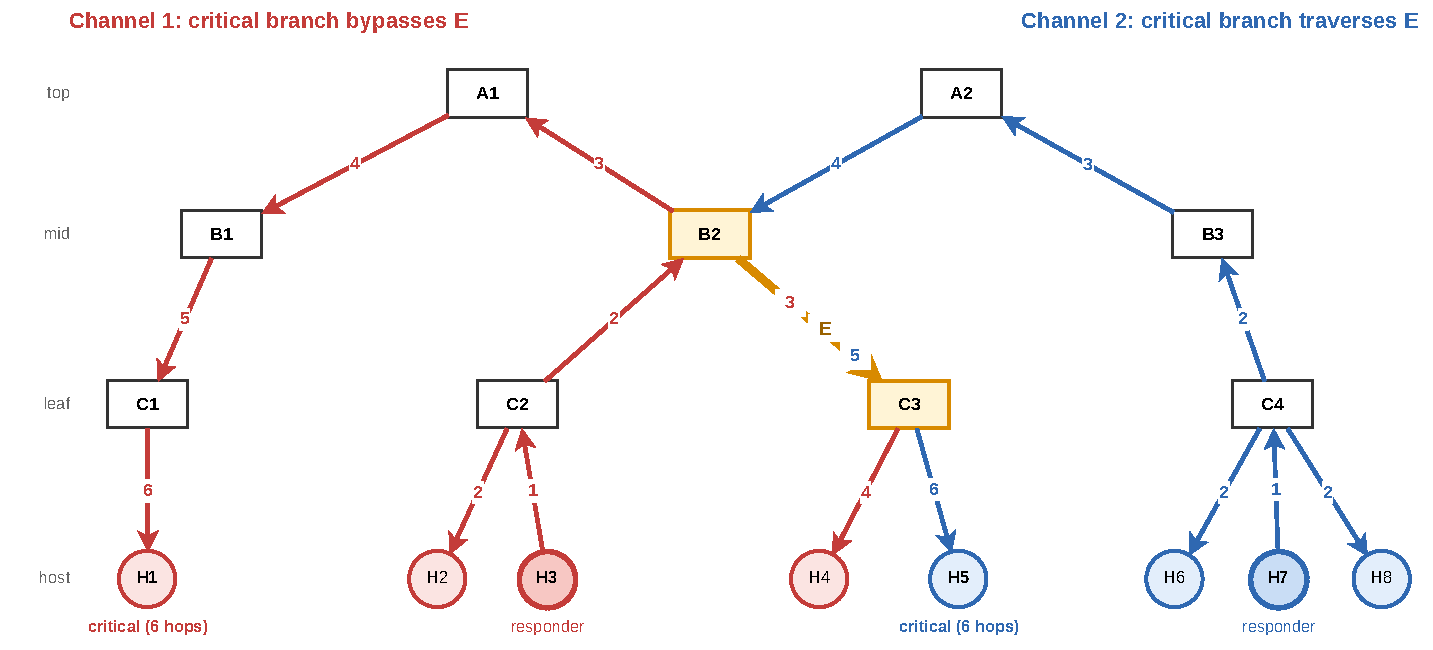
\includegraphics[width=0.94\linewidth]{img/eval/asym_2348.pdf}
\caption{\texttt{asym-2348}：用 responder 放置改变同一条队列在完成
反馈中是否可见。橙色为被测 egress $E$；配对放置保持成员、流量和 $E$
不变，仅 responder 位置使最慢分支绕过 $E$（红）或经过 $E$（蓝）。}
\label{fig:asym-2348}
\end{figure*}

\parab{过滤的公平性代价取决于控制律.}
最后，我们在同一 $E$ 上运行两个持续 backlogged 的四-rank channel。
两个 placement 采用共同的 $[1.92,5.76)$~ms 墙钟测量窗，并在 5.76~ms
同时停止发放新 offset 后排空所有已发 credit。主指标只计 completion
timestamp 落入该固定窗口的 logical bytes，不再使用各 job 自身的
submit-to-finish span，因而不包含先完成者独占的尾段。

\begin{table*}[t]
\centering
\caption{共享链路 $E$ 的反馈可见性对公平性与链路效率的影响。每个指标
的两列中，两条 channel 的流量均经过并竞争同一个 $E$：one-sided
feedback 表示只有 Channel~2 的 max-completion feedback 能感知 $E$ 上
的排队，two-sided feedback 表示双方的 feedback 都能感知。Channel~1
share 的 50\% 表示均分；aggregate completed goodput 把相同固定窗口内
两条 channel 完成的 logical bytes 相加后除以窗口长度，不再归一化。
DCQCN-style 使用 20 个 paired RNG run，其 Channel~1 share 唯一非零的
Student-t 95\% CI 为 0.003 percentage points；其余控制器的事件序列
确定，各运行一次。}
\label{tab:cc-asym}
\small
\pgfplotstabletypeset[
  col sep=comma,
  columns={controllerLabel,hiddenShare,visibleShare,
    hiddenAggregateGbps,visibleAggregateGbps},
  columns/controllerLabel/.style={
    string type,column name={Controller},column type=l,
  },
  columns/hiddenShare/.style={
    column name={One-sided feedback},
    fixed,fixed zerofill,precision=2,column type=r,
  },
  columns/visibleShare/.style={
    column name={Two-sided feedback},
    fixed,fixed zerofill,precision=2,column type=r,
  },
  columns/hiddenAggregateGbps/.style={
    column name={One-sided feedback},
    fixed,fixed zerofill,precision=1,column type=r,
  },
  columns/visibleAggregateGbps/.style={
    column name={Two-sided feedback},
    fixed,fixed zerofill,precision=1,column type=r,
  },
  every head row/.style={
    before row={
      \toprule
      & \multicolumn{2}{c}{Channel~1 share of completed goodput (\%)}
      & \multicolumn{2}{c}{Aggregate completed goodput (Gbps)}\\
      \cmidrule(lr){2-3}\cmidrule(lr){4-5}
    },
    after row=\midrule,
  },
  every last row/.style={after row=\bottomrule},
]{plots/data/pgf/cc.csv}

\end{table*}

\Cref{tab:cc-asym} 中，one-sided feedback 下 Swift 获得 93.0\% 的
completed goodput；改为 two-sided feedback 后，其 share 回到 50.0\%，
两种放置下的 aggregate completed goodput 分别为 199.0 和
198.6~Gbps——强烈的份额偏置来自瓶颈容量的重新分配，而非共享链路
空闲。Oscar 和 TIMELY 的 share 变化分别为 4.81 和 3.91 percentage
points，低于预注册的 5-point``明显偏置''门槛，我们不把它们写成强公平
性失效；其中只有 TIMELY 的 aggregate completed goodput 同时从 182.3
提高到 198.6~Gbps。DCQCN-style 的两个 placement 分别为
$49.975\pm0.003$\% 和 50.000\%，近似不受放置影响。全部 46 次运行均无
PFC 或协议错误。因此，branch-slack filtering 是信号本身的确定性边界，
但它是否放大为可见的带宽偏置取决于控制律；在该构型中，只有 Swift 达到
预注册的强边界阈值。

\section{可靠性}
\label{ssec:eval-reliability}

\parab{物理 communicator 生命周期.}
固定-$N=4$ 实验在五个新进程中交替创建和销毁 group~0/1，每个进程运行
25 轮，共验证 500 个 communicator 和 2,000 个 rank lifecycle。rank-churn
实验保持四个物理 rank、两个 poller、EAL 进程、NIC 队列和 FPGA 镜像不变，
在 group~0/3 上交替 $N=4$ 与 $N=2$，再次验证 500 个 communicator 和
2,000 个 rank lifecycle。两组实验均无残留 completion state、结构错误、
Tofino/DCMAC 错误、accelerator configuration write 或 image reload。
该结果验证 endpoint-only 建组、销毁和 message epoch 复用，不作吞吐或
建组时延声明。

\parab{物理故障证据边界.}
归档的三-rank DPDK fault-proxy 实验对七种定向竞态各运行五次，35 个
attempt 全部得到 105/105 个 PASS rank，覆盖相应 endpoint state
machine；但该实验早于最终 endpoint 源码，其三-NIC proxy 布线也已被
V80 拓扑替换。当前单层与两层镜像在正式运行中都实际执行过一般
recovery，但没有重跑这七种精确注入；本文因此不把旧 proxy 结果当作当前
routed 实现的定向故障验收，完整故障矩阵由以下包级实验给出。

包级仿真部分在 U200 上固定 16 ranks、单 job、单树、256-MiB message、
Swift 和 65,536 slots，只注入丢包、straggler 或 requester crash。
normal credit 的 cutover deadline 和 repair trigger/END 的 RTO 均为
10~ms，timeout 敏感性实验单独改变前者。结果量化所测有限故障下的恢复
代价和正确性边界。

\parab{有限丢包均能完成，但 repair 很快成为主成本.}
我们在 host-facing 和 tree 链路的两个方向独立注入 per-hop Bernoulli
loss，每个非零点包含 20 个 RNG run；实际 drop denominator、packet
class 和有向链路计数在每次运行中闭合。安装 loss model 但令 $p=0$
时，goodput 为 180.9~Gbps。\Cref{fig:loss} 显示，$p=0.01\%$ 时两个
scope 分别达到 $62.7\pm5.3$ 和 $65.8\pm4.7$~Gbps；$p=1\%$ 时约
27.6\% 的 offset 由 repair 提交，goodput 降至 4.10~Gbps，逐跳 wire
bytes 相对 $p=0$ 增加约 60.5\%。5\% 压力点仍全部完成，但 repair 比例
达到 80.6--80.7\%，goodput 只剩 0.78--0.81~Gbps。

\begin{figure*}[t]
\centering
\resizebox{\linewidth}{!}{%
\begin{tikzpicture}
\begin{groupplot}[
  group style={group size=2 by 1,horizontal sep=1.25cm},
  arbor axis,arbor panel,
  width=8.0cm,height=4.7cm,
  xmode=log,
  xmin=0.006,xmax=7,
  xtick={0.01,0.1,1,5},xticklabels={0.01,0.1,1,5},
  xlabel={Per-hop packet loss (\%)},
]
\nextgroupplot[
  title={(a) Logical goodput},
  ylabel={Goodput (Gbps)},ymin=0,ymax=75,
  ytick={0,25,50,75},
  legend to name=g6losslegend,legend columns=2,
  legend style={/tikz/every even column/.append style={column sep=5pt}},
]
\addplot[ArborBlue,thick,mark=*,error bars/.cd,y dir=both,y explicit]
  table[col sep=comma,x=loss_pct,y=host_goodput_gbps,
    y error=host_goodput_ci95]
  {plots/data/pgf/reliability.csv};
\addlegendentry{Host-facing links}
\addplot[ArborOrange,thick,dashed,mark=square*,
  error bars/.cd,y dir=both,y explicit]
  table[col sep=comma,x=loss_pct,y=tree_goodput_gbps,
    y error=tree_goodput_ci95]
  {plots/data/pgf/reliability.csv};
\addlegendentry{Tree links}

\nextgroupplot[
  title={(b) Recovery work},
  ylabel={Offsets committed by repair (\%)},ymin=0,ymax=90,
  ytick={0,20,40,60,80},
]
\addplot[ArborBlue,thick,mark=*,error bars/.cd,y dir=both,y explicit]
  table[col sep=comma,x=loss_pct,y=host_repair_pct,
    y error=host_repair_ci95]
  {plots/data/pgf/reliability.csv};
\addplot[ArborOrange,thick,dashed,mark=square*,
  error bars/.cd,y dir=both,y explicit]
  table[col sep=comma,x=loss_pct,y=tree_repair_pct,
    y error=tree_repair_ci95]
  {plots/data/pgf/reliability.csv};
\end{groupplot}
\node[anchor=south,yshift=26pt] at (group c1r1.north east)
  {\ref{g6losslegend}};
\end{tikzpicture}%
}

\caption{Host-facing 或 tree 链路双向独立随机丢包下的 20-run 均值和
Student-t 95\% CI。概率是每条所选有向链路上 eligible Arbor packet 的
per-hop loss；5\% 为压力点。}
\label{fig:loss}
\end{figure*}

\parab{Cutover deadline 过短或过长都会增加完成时间.}
我们丢弃一份 master，并交叉扫描 $\{2,10\}\times p99$ clean RTT 和固定
50-ms deadline，以及 $\{0,0.5,2\}\times p99$ requester delay；repair
RTO 始终固定为 10~ms。$2\times p99$ 把 32,682--32,768 个 offset 提前
转入 repair，goodput 为 68.5--68.9~Gbps；$10\times p99$ 只触发
129--175 次 repair，达到 173.5--185.7~Gbps。50-ms deadline 只 repair
丢失的那一个 offset，但 CCT 被该 deadline 拉长到 50.1~ms。normal
cutover 和 repair 重传因此必须使用独立 timer。

\parab{定向竞态保持单次提交.}
仿真侧的 18 个 packet-level 用例覆盖六种原语，以及 master、
payload+credit、\texttt{REGISTER\_ACK}、\texttt{END}/\texttt{END\_ACK}
和 repair trigger 的丢失、重复或迟到。跨级 master 丢失产生一次
repair trigger 和一次 repair commit；Broadcast 和 AllGather 的 push
offset 已在首发时 self-commit，丢失接收副本只重放 payload，没有二次
commit。一条 tree branch 暂停 2~ms 时，112 个 offset 转入 repair，
运行仍以 72.5~Gbps 完成。把一个 requester 限制到线速的 50\% 和
10\% 时，整组 goodput 分别为 97.4 和 19.8~Gbps；永久 crash 在
100~ms 截止前不提交缺少输入的结果。272 个有限故障点全部完成，且没有
PFC、\texttt{AGG\_MISS}、live overwrite 或协议违例；crash 边界不计入
成功均值。

\section{局限性}

评估有五项边界。第一，ns-3 不执行 payload 数值运算；其结果验证协议、
状态和链路线量，不能替代物理 FPGA 的 FP32 正确性、吞吐或资源证据。
第二，该 ns-3 fork 把 PRE 副本逐份计入同一 ingress queue；PFC pause 是
仿真中的真实事件，其 headroom 不能直接解释为商用交换机所需的物理
buffer。第三，没有一种端侧拥塞控制算法及参数配置在所有 group size、
拓扑和并发度上同时最优；正文参数按实验族在独立 calibration 上冻结，并
统一用于该实验族的 evaluation seed。第四，物理原型只有一块 V80、四个
rank 和每端口 100-GbE 的线速上限；正式性能运行以物理锁和进程门排除
ns-3、Vivado/JTAG 及其它 endpoint workload，所得 routed timing、资源和
吞吐不能外推为生产集群结果。第五，ATP-8K 和 SwitchML-8K 是按论文数据面
语义构建的独立 FPGA/endpoint 实现，不是原作者代码；物理结果支持相同
testbed 上的实现比较，不证明对原系统所有功能和优化的复现。当前 routed
镜像尚未重跑七种精确故障注入；两层动态选路虽有物理消融，但硬件计数器只
支持 500-ms 时间分辨率，控制律替换与更细响应时间仍采用包级仿真证据。

\FloatBarrier

\chapter{大模型训练评估}
\label{chap:llm-evaluation}

\Cref{chap:simulation} 分别隔离了共享聚合状态、逐-offset 选树、拥塞控制和
恢复机制。本章把这些机制放回带计算依赖的训练计划，报告 FSDP 阶段窗口和
4D final-microbatch backward tail 的完成时间。两类结果均来自直接包级仿真；
backward tail 的边界从所有 rank 到达冻结的 entry barrier 开始，到所有 rank
完成 exit barrier 为止，不外推为完整 optimizer step。

% TODO(testbed-v80-gpu): 在正式硬件实验完成后，于本章开头增加一节物理
% GPU/PyTorch 训练片段。固定四 rank、每 rank 一张 GPU/NIC、相同模型片段与
% optimizer 边界，报告 GPU-resident tensor 的端到端时间、Arbor 与未加速
% backend 的配对加速比、正确性和流水线分解。第五章只报告 transport/core/
% FPGA 指标；这里不重复其吞吐微基准。已有的“双 GPU 分片到单 NIC”工程 smoke
% 不作为该训练拓扑的结果。

\section{实验设置与比较边界}
\label{ssec:llm-setup}

\parab{拓扑与运行.}
本章使用两个冻结的 2,048-GPU Clos。8B FSDP phase-window 保留
4:1 配置：host、ToR--leaf 和 leaf--spine 链路均为 400~Gbps。
70B Classic 3D 及 405B direct-tail 矩阵使用固定 2:1 配置：64 个 ToR、
16 个 leaf 和 8 个 spine，每个 ToR 连接 32 张 GPU；host 链路为
400~Gbps，ToR--leaf 和 leaf--spine lane 为 800~Gbps，逐链路时延为
3~\textmu s。物理 packet buffer 为 128~MiB，每个聚合 slot 承载
8-KiB payload；各 workload 的聚合容量在相应小节单独给出。包级网络开启
ECN 和 PFC；PFC 只提供无损保护，结果同时审计 ECN、pause、drop、最终队列
和协议状态。

\parab{指标与重复.}
H100 计算时间来自冻结的 analytical roofline，而非实测 GPU trace。确定性
实验使用 seed 1。FSDP phase-window 每点运行一个 warm-up、一个 measured
和一个 cooldown iteration；matched-granularity direct-tail 矩阵运行一个
warm-up 和一个 measured iteration，不再启动 cooldown。两类实验均只有一个
measured observation，不生成统计误差条。

\parab{比较口径.}
本文以 compute-inclusive phase completion 或 backward-tail completion
比较系统。collective logical goodput 用完整输出 tensor 大小除以完成时间；
其分子不含链路复制和 header，不能解释为物理链路带宽。对 $N$-rank NCCL
ring，AllGather/ReduceScatter 的 bus bandwidth 等于 logical goodput 乘以
$(N-1)/N$，AllReduce 则乘以 $2(N-1)/N$。因此，DP4 AllGather 的
524.05~Gbps logical goodput 对应 393.04~Gbps bus bandwidth，没有超过
400-Gbps 链路线速。多 job 实验的 job 使用互斥 GPU 集合；direct
backward-tail 实验还固定模型、batch、并行维度、rank placement 和计算 DAG，
只替换 scale-out collective 的实现。

\parab{Scale-up 与 scale-out 分开控制.}
FSDP phase-window 实验保留两个 NCCL 对照。NCCL-flat 让全部 128 个 rank
直接通过 Ethernet 执行 collective；NCCL-NVLink 先在每个八 GPU 节点内执行
RS/AG，再让八个 16-node shard 并行使用 scale-out 网络。Arbor 行不包含
NVLink 阶段，128-rank AllGather 和 ReduceScatter 全部由 Arbor 在
scale-out fabric 上完成。因此，该实验给 NCCL 保留了更强的本地层次，但
不构成两种系统共享同一 scale-up 通路的比较。direct-tail 实验为所有系统
固定相同的 node-local TP/NVLink 与 PP 点对点通路，只改变跨节点 collective。

\parab{Baseline 拥塞控制.}
NCCL 及 ATP/SwitchML hybrid 的 scale-out RDMA 均启用 packet-level DCQCN。
DCQCN 只作用于这些 RDMA/P2P QP；ATP 的网内聚合流量使用其 ECN-AIMD
窗口，SwitchML 的聚合流量不包含端侧速率控制，两者均不继承 DCQCN。
\Cref{app:sim-models} 给出预先声明的有限调参预算；每类 workload 只在该预算内
选择 profile，并在新的随机运行上通过 held-out 检查后冻结。正式运行同时核对
DCQCN 配置、QP 实际降速、ECN、PFC、drop 和最终队列排空。该流程避免以默认或
未生效的拥塞控制代表 baseline，但不声称搜索得到 DCQCN 的全局最优参数。所有
P2P QP 中最低的测量期平均速率达到 400-Gb/s 线速的 95\% 时，记为无实质降速；
瞬时最小速率、ECN 和队列状态仍单独报告。

\parab{聚合状态.}
FSDP phase-window 的 Arbor 运行使用 65,536 个 slot 的非约束观测池，避免
选定控制参数时混入容量不足。全部正式 Arbor 点中，最大 live occupancy 为
9,293 slots，最大 allocation-sequence reuse depth 为 13,993 slots；随后
冻结的 16,384-slot（128-MiB）统一容量高于该观测深度。这个检查说明
128~MiB 对已运行 trace 足够，但 phase-window 数字仍来自配置 512~MiB
观测池的原始运行，而不是一次事后标记为 128~MiB 的重跑。

\section{FSDP 阶段窗口}
\label{ssec:llm-fsdp-windows}

该实验从 Llama-3.1-8B 的 128-rank weight-sharded 训练 DAG 中截取两个原生
窗口：forward 使用第 15 层的 compute 与 AllGather，backward 使用第 15、
14 层并保留 prefetch-distance-1 的 AllGather/ReduceScatter 重叠。每个
job 的计算节点、tensor 大小、通信组和依赖在三个 backend 间完全一致；
$J\in\{1,4,8,12,16\}$ 只改变共享同一 Clos 的独立 job 数。结果衡量这些
窗口的完成时间，不外推完整训练 step、MFU、收敛速度或 time-to-accuracy。

\begin{table*}[t]
\centering
\small
\caption{Llama-3.1-8B FSDP compute-inclusive phase completion。时间单位为
ms；speedup 为 NCCL-NVLink 时间除以 Arbor 时间，大于 1 表示 Arbor 更快。
每点包含一个 measured iteration。}
\label{tab:llm-fsdp-phase}
\begin{tabular}{llrrrr}
\toprule
阶段 & $J$ & Arbor & NCCL-flat & NCCL-NVLink &
Arbor speedup vs. NVLink \\
\midrule
Forward  & 1  & 10.376 & 11.143 &  7.581 & 0.731$\times$ \\
         & 4  & 10.376 & 11.143 &  7.517 & 0.724$\times$ \\
         & 8  & 10.377 & 11.143 &  9.262 & 0.893$\times$ \\
         & 12 & 10.377 & 16.485 & 12.082 & 1.164$\times$ \\
         & 16 & 10.379 & 19.903 & 12.413 & 1.196$\times$ \\
\midrule
Backward & 1  & 50.142 &  55.487 & 35.251 & 0.703$\times$ \\
         & 4  & 50.142 &  55.487 & 37.566 & 0.749$\times$ \\
         & 8  & 50.195 &  55.488 & 53.360 & 1.063$\times$ \\
         & 12 & 51.083 & 100.682 & 63.505 & 1.243$\times$ \\
         & 16 & 51.254 & 108.257 & 72.299 & 1.411$\times$ \\
\bottomrule
\end{tabular}
\end{table*}

\Cref{tab:llm-fsdp-phase} 显示，低并发时 NCCL-NVLink 的本地层次降低了
phase time：forward 在 $J\leq8$、backward 在 $J\leq4$ 均快于不使用
NVLink 的 Arbor。随着共享 scale-out fabric 上的 job 数增加，Arbor 的
phase time 变化较小，并分别在 forward 的 $J=12$ 和 backward 的 $J=8$
越过 NCCL-NVLink。$J=16$ 时，Arbor 的 forward 和 backward 分别快
$1.196\times$ 和 $1.411\times$；相对 NCCL-flat 则分别快
$1.918\times$ 和 $2.112\times$。在该配置范围内，node-local collective
降低了低竞争时延，但没有消除高并发下 scale-out collective 对 phase time
的影响；这些结果不说明 Arbor 使用了或替代了 NVLink。

\section{405B 4D-FSDP backward tail}
\label{ssec:llm-405b-fourd-fsdp}

405B 4D-FSDP workload 使用 Llama-3.1-405B、8,192-token sequence、TP8、PP8、
CP2 和 DP16，共 2,048 张 GPU；多租户配置把 DP 缩为 4，使每个 job 使用
512 张互斥 GPU。所有系统复用相同的 node-local TP/NVLink、PP 点对点通信、
计算 DAG 和 placement。Arbor 直接执行 scale-out AllReduce、AllGather 和
ReduceScatter；ATP 与 SwitchML 只执行其支持的 scale-out AllReduce，其余
scale-out collective 使用相同的 NCCL-flat/RDMA fallback。该 hybrid 对照
把 AllReduce-only INC 的收益与 Arbor 的多原语支持分开。

Arbor 按通信组规模选择 AllGather 注入方式。单 job 的 DP16 依次执行各
owner 的广播，避免多个 owner 同时向同一接收端汇聚；多 job 的 DP4 允许
四个 owner 并发，并把每个 owner 的每 subchannel 速率设为
$B/((N-1)S)$，使每个接收端的三路输入之和不超过 400~Gbps。DP4 使用独立的
Swift profile（window 96、target queue 20~\textmu s、$\beta=0.05$、
$AI=0.5$），DP16 保留顺序语义及原 profile。独立的 forward 与 backward
DP4 包级运行均达到 490.961~Gbps logical goodput，即 368.221~Gbps bus
bandwidth；两点均为零 PFC、drop 和 repair，结束时队列与聚合状态清空。

多租户配置在运行前一次登记四个租户，并在 $J=1,2,3,4$ 间保持同一
SwitchML 分区。已声明 communicator 在 ToR、leaf 和 spine 上的逐交换机
demand 分别为 48、128 和 64，leaf 是约束层；两个不可借用 physical set
把 16,384 个 slot 等分为每棵树每 set $Q=64$。leaf 上只经过 sharded-DP
树，因此即使管理员按 collective 类别离线分配，CP 树释放的状态也不能扩大
该约束层上的 DP window。未活跃租户的分区不被借用，故 $J=1$ 同样包含为
四租户声明上限预留状态的代价。

正式评估直接运行冻结 DAG 的 final-microbatch backward tail。U1/DP16 使用
全部 2,048 张 GPU；U4/DP4 在同一四租户预注册 universe 下运行
$J=1,2,3,4$，其中 $J=1$ 是静态预留已经发生但尚无租户竞争的诊断 control，
$J=2,3,4$ 构成多租户曲线。$J=3$ 在其余点完成后释放，不参与协议或参数选择。
每点保留原生 compute、TP、CP、PP、AllReduce、AllGather 和 ReduceScatter
依赖，并审计全部 DAG 节点、通信字节、ECN、PFC、drop、DCQCN 实测速率、
聚合状态和最终队列。早期稿件使用单独 calibration 得到的 operation 时延
重新调度完整 step；DP4 AllGather 语义修正后，这批组合结果已作废。

% DIRECT 405B TAIL RESULT PLACEHOLDER (2026-08-20): insert the U1 and
% U4/J={1,2,3,4} four-system table only after all direct packet runs pass the
% streamed DAG/runtime/protocol audit and the 40-point paper-data join.

\section{70B Classic 3D：隔离 scale-out AllReduce}
\label{ssec:llm-70b-classic-threed}

该实验回答一个更窄的问题：当训练 DAG 中由 backend 选择的 scale-out
collective 只有 AllReduce 时，Arbor 相对 NCCL、SwitchML 和 ATP 的
compute-inclusive tail 收益是多少？workload 使用 Llama-3.1-70B、
8,192-token sequence、microbatch 1、gradient accumulation 32 和 1F1B。
三个并行维度固定为 TP8、PP16 和 DP，CP 为 1；U1、U4 和 U8 分别取
DP16、DP4 和 DP2，因此每个 job 使用 2,048、512 和 256 张 GPU。
四种系统共享计算 DAG、node-local TP/NVLink、PP RDMA、placement 和
arrival time；只有 FP32 gradient AllReduce 的 scale-out backend 不同。
该控制避免把 SwitchML/ATP 不支持 AllGather 或 ReduceScatter 的 fallback
代价计入比较，但 tail 仍包含各系统共有的计算和非 scale-out 通信，因而不是
孤立的 AllReduce 微基准。

正式矩阵包含五个 cell：U1/J1，以及 U4 的 $J=1,4$ 和 U8 的 $J=2,8$。
后两组分别构成 25\% 和 100\% active-GPU 的匹配对照：
$1\times512$ 对 $2\times256$，以及 $4\times512$ 对 $8\times256$。
从 U4 到 U8，active communicator 数分别由 128 增为 256、由 512 增为
1,024；总 active GPU 和 aggregate DP replica 数保持不变，但 DP group size
从 4 变为 2，因此该对照同时包含通信粒度变化。每个 aggregation-capable
switch 为所有 INC 系统固定 64~MiB，即 8,192 个 8-KiB slot；SwitchML
使用预先冻结的双 physical-set 静态分区（$Q=32$），未活跃 communicator
的分区不可借用。Arbor 的 PP/collective work-conserving 调度约定见
\cref{app:classic-pp-scheduler}。

冻结 DAG 直接执行 final-microbatch backward tail；mb0--mb30 的已完成累积
状态由 all-rank entry barrier 表示。每个 cell 先运行一个 warm-up tail，
再运行一个 measured tail。主指标从 measured entry barrier 的最晚 rank
ready 开始，到最晚 active tenant 完成为止；多租户平均值只作描述性统计，
不充当独立重复。

\begin{table*}[t]
\centering
\small
\caption{70B Classic 3D final-microbatch backward-tail completion。时间单位
为 ms，越低越好；主指标取 active tenant 的最大完成时间。``最快 baseline''
在 NCCL、SwitchML 和 ATP 中逐 cell 选择，最后一列为 Arbor 相对它的时间
降幅。每个 cell 包含一个 measured iteration。}
\label{tab:llm-classic3d-tail}
\setlength{\tabcolsep}{3.5pt}
\resizebox{\linewidth}{!}{%
\begin{tabular}{llrrrrlr}
\toprule
Cell & jobs$\times$GPUs/job & Arbor & NCCL & SwitchML & ATP &
最快 baseline & 降幅 \\
\midrule
\inputtabularbody{plots/data/pgf/classic3d-2to1-table-body.tex}
\bottomrule
\end{tabular}}
\end{table*}

\Cref{tab:llm-classic3d-tail} 中 Arbor 在五个 cell 均最快，完成时间为
349.960--376.935~ms。相对 SwitchML，Arbor 将 tail 缩短
21.8\%--27.2\%；相对 NCCL 和 ATP 的降幅分别为 20.5\%--39.5\% 和
13.9\%--81.5\%。若逐 cell 只比较最快 baseline，降幅仍为
13.9\%--27.1\%。ATP 的 U1/J1 点为 1,935.962~ms，并同时出现 4,085 次
PFC pause；表中保留该 return-zero、最终排空的异常慢点，而不截断或以其它
运行替换。

匹配对照没有显示 SwitchML 随 communicator 增多而退化。25\% load 下，
U8/J2 相对 U4/J1 的 completion ratio 在 Arbor 和 SwitchML 上分别为
0.998 和 0.999；100\% load 下分别为 0.998 和 1.001。该结果说明本 workload
中的静态分区尚未成为 SwitchML 的可见瓶颈；它支持五个 cell 上的端到端
AllReduce-backend 比较，但不能单独证明 Arbor 的收益来自动态 SRAM 共享。
同时，由于 U4/U8 还改变 DP group size，这两个 ratio 只作为匹配负载下的
粒度敏感性结果，不作单变量因果解释。

所有 Arbor cell 均为零 PFC、零 drop、零 protocol violation 和零 timeout，
结束时队列与 live aggregation state 清空。U4/J4 并非零 miss：它记录
5,656 次 aggregation miss、5,528 次 repair trigger 和同数 repair commit，
最终 live slot 为 0。因而该点表明 repair 在这条 trace 上完成了恢复，而不
表明 64~MiB 消除了所有容量压力。每个 cell 只有 seed 1 的一个确定性重复；
此外 U4/J1 Arbor 是冻结调度方法时使用并随后按 exact-run 身份提升的 canary，
不是独立 held-out 重复。这些数字限定为该 direct tail，不外推完整 optimizer
step、MFU 或 time-to-accuracy。

\chapter{相关工作}
\label{chap:related}

\section{集合通信运行时}

NCCL~\cite{nccl} 和 Gloo~\cite{gloo} 使用 ring、tree 和分层算法实现常用集合
通信。MSCCL~\cite{msccl}、HiCCL~\cite{hiccl} 和 TACCL~\cite{taccl} 进一步
允许编译器或用户组合发送、接收、规约和拷贝动作。这些系统决定数据如何分块及
依赖如何调度，底层传输仍接收点对点操作。\sysname 不替换 collective schedule；
它为 schedule 提供多播-聚合流，使同一 packet offset 的输入在网络中保持共同的
路径、聚合和恢复边界。

\section{在网集合通信}

SwitchML~\cite{switchml} 在可编程交换机中执行规约，并按任务划分聚合状态；
NetReduce~\cite{netreduce} 在 NIC-FPGA 的 RDMA 路径中聚合；SHARP~\cite{sharp}
由控制面建立硬件 reduction tree。这些系统以任务级资源映射隔离并发聚合。
ATP~\cite{atp} 改用共享 slot 和数据面哈希，并在冲突时由参数服务器补全；
A2TP~\cite{a2tp} 与 PA-ATP~\cite{paatp} 分别改进公平性和进度调度。AIRP~
\cite{airp} 则根据全局视图规划网络中的聚合资源。

EPIC~\cite{epic} 把交换机暴露为传输端点，可以在交换机终结连接，也可以让端点
发起的传输状态经交换机翻译到后续链路。\Cref{ssec:inc-limits} 按组外端点、连接
终结和连接翻译归纳这些组织方式。它们分别解决资源分配或连接推进，但 packet
路径、聚合位置和恢复状态仍由不同连接或控制过程维护。\sysname 用一份组播 credit
绑定 packet offset、subchannel 和逐级 slot。responder 用整组完成事件更新拥塞
控制，并在超时或 owner mismatch 时启动整组 repair。

\section{Receiver-driven 传输与拥塞控制}

Homa~\cite{homa}、NDP~\cite{ndp} 和 ExpressPass~\cite{expresspass} 由接收端
发放 grant 或 credit，以限制发送端注入。\sysname 同样把发送许可放在接收端，
但一份 credit 同时授权 requester group 对一个 packet offset 各发送一份输入。
该许可还指定 subchannel，并在返回路径取得聚合位置；普通 unicast grant 不需要
维持这些组内一致性条件。

DCTCP~\cite{dctcp}、DCQCN~\cite{dcqcn}、HPCC~\cite{hpcc} 和 TIMELY~
\cite{timely} 分别使用 ECN、INT 或 RTT 调节发送窗口和速率。\sysname 不固定
控制律，而是在 responder 提供 rate/window 两道 credit gate。基于时延的算法
读取整组 fan-in 的完成时间；ECN 算法读取各分支 CE 的 OR。该接口改变反馈的
聚合范围，但保留所选控制律自身的收敛和公平性限制（\cref{ssec:cc}）。

\section{多路径传输}

ECMP~\cite{ecmp} 按 flow 哈希路径；CONGA~\cite{conga}、Hermes~\cite{hermes}、
Presto~\cite{presto} 和 LetFlow~\cite{letflow} 根据网络状态在 flowlet 或 packet
粒度切换路径。Themis~\cite{themis} 使用确定性的 PSN--path 映射，在 commodity
RNIC 的重传语义下支持 packet spraying，并用基于乱序程度的信号暂时避开检测到
的慢路径或失效路径。MRC~\cite{mrc,mrcsrv6} 定义 per-connection EV 集合和
sender-side congestion-control 信号，并把具体 load-balancing algorithm 留给
实现；其生产实现逐 packet 轮转 active EV，临时避开带 ECN 的 EV，并在路径丢包
后替换 EV。这些机制以单个 unicast packet 或 flow 为调度对象。

\sysname 为每棵预装 subchannel 维护独立的 rate/window gate，并把后续 offset
分配给当前允许发放的候选。该选择器可以调度单个 packet；用于在网 fan-in 时，
一次决定覆盖同一 packet offset 的整组输入。整组完成事件更新所选 subchannel
的 gate，使后续 offset 只在当前允许发放的聚合树间分配。

在网 fan-in 另有一项正确性条件：同一 packet offset 的全部输入必须选择同一
聚合树，并在共享子树中命中同一 slot。\sysname 由 responder 选择 subchannel，
再通过组播 credit 把选择复制给全部 requester；已发出的 Credit Context 不迁移。

\chapter{总结}
\label{chap:conclusion}

\sysname 用独立的 rate/window gate 表示预装 subchannel，并以反馈门控选择器逐
packet offset 分配路径。用于在网 fan-in 时，组播 credit 把所选 subchannel 和
逐级聚合位置绑定到整组 requester，使通信组内的输入共享 Credit Context。
responder 根据整组完成事件控制后续 credit，并在超时或 owner mismatch 时启动
整组 repair。该传输对象使 packet-level 路径选择、聚合状态、拥塞反馈和恢复
使用相同边界。
六种集合通信原语只改变 channel 集合和 payload 方向，传输与恢复规则保持不变。

Normal credit 在带内推进各级共享循环 allocator，并把位置压栈返回；加速器
从 request 的位置栈直接访问共享 slot，并用 owner 隔离轮转后的迟到输入。
Normal request 单注入使数据面只需计数；requester 身份和 repair 去重保留在
responder。循环 allocator 的根本条件是 $A_e\geq D_e$，其中 $D_e$ 包含同一
domain 的全部 normal advance。严格 all-advance envelope 给出
$\lceil B_e+\lambda_eR_e\rceil$ 充分界；
把每个 fixed-$P$ data context 与一份 payload packet 一一对应，可得到通用
$2R_e$ 端口界，full-payload carrier 再收紧为 $R_e$。端口界对实际推进同一 allocator 的端口
求和，不随 job 数或 rank 数额外放大。
当 $A_e=D_e$ 时，带内循环分配以最小安全深度运行，并使 100\% 的已配置地址
成为无提前复用冲突的有效容量，不受哈希冲突或 per-job 分区影响。

包级仿真验证了共享状态、反馈驱动的逐-offset 选树、四种端侧拥塞控制算法和
故障恢复。在四棵候选树依次受限的
单-job 实验中，dynamic 达到 190.0~Gbps，而全程最优固定配额为
154.6~Gbps；前者在 4--5.5 个反馈周期内完成迁移。状态实验
分别覆盖共用端口和端口分散的 switch-wide allocator；110 次运行均满足相应
的循环复用界。在固定 32$\times$200-Gbps spine 和按端口界配置的 42-MiB
状态上，我们将配置人口从 16 增至 512，并令约 75\% 的 job 持续通信；相对
各点由拓扑确定的 per-job service budget，\sysname 保持 97.42\%--97.98\%，
静态分区的 SwitchML-like 在分区成为瓶颈后为 69.99\%--75.03\%，ATP-like
随哈希冲突增加从 97.59\% 降至 40.50\%。在 200-Gbps 一、二、三层拓扑
中，单-job 256-MiB AllReduce 分别达到 196.25、197.17 和
195.83~Gbps；50\%-active 的八-job 轨迹中，两/三层 aggregate goodput
为 763.96 和 754.97~Gbps，相对最优静态 SwitchML-like 提高
17.0\% 和 15.6\%。
当前 ns-3 模型不执行 FP32 运算，
1024-host 结果也只验证协议和状态路径。

% TODO(testbed-v80-final): 补最终四 rank V80 FP32、端侧 core、ATP/SwitchML、
% 资源/功耗与 GPU/PyTorch 训练片段结论；不要恢复旧三 rank DPDK proxy 数字。


\bibliographystyle{plain}
\bibliography{ref}

\appendix

\chapter{物理原型实现与 baseline 调优审计}
\label{app:physical-implementation-audit}

\parab{CPU 资源口径.}
每次正式运行记录 rank、角色、poller 数、EAL lcore、NUMA socket、NIC 队列和
内存放置。正文以执行协议数据面的已配置 poller lcore 为资源单位；只负责
发布 collective 和等待完成的 EAL main lcore 不计入该指标。四台主机在运行前
固定 performance governor，并对实际选用的 lcore 逐核核对；不满足 governor、
NUMA、进程互斥或链路门禁的运行不进入正式统计。我们不使用进程生命周期上的
CPU-time 比值，因为初始化、测量和退出阶段的分母并不对应同一数据面窗口。

\parab{镜像绑定与两层参数.}
正式绑定为：Arbor 单层结果使用 r81 镜像，细粒度物理状态扫描与其后的
端侧 fast-path 实验使用通过同等 route/timing 门的 r88；ATP-8K 与
SwitchML-8K 分别使用独立的 r87 和 r79；两层实验使用 r60。两层实验固定
Swift target 40~\textmu s、$W_0=2$、cap 16、8-\textmu s startup
stagger、12-credit shared window 和 200-\textmu s stall repair；端点
日志中的 \texttt{slot\_pool\_size=1024} 只是可动态映射的逻辑标识
空间，不计作物理 row。归档 fault-proxy 批次的 35 个成功 attempt 之外，
另有三个 attempt 在发包前因基础设施 preflight 被拒，不计入成功统计。

\parab{Baseline 优化边界.}
ATP-8K 与 SwitchML-8K 使用各自独立的端侧协议状态机和 FPGA 镜像。端侧候选
包括 borrowed RX、NUMA-local payload、每 poller 独立队列、批处理、状态查找
快速路径和多段 TX；每个候选先通过 exact-FP32、RX/TX 守恒和 poller 所有权
检查，再用独立 engineering pilot 判断是否保留。无收益或降低吞吐的候选仍
保留源码、命令和原始日志，不从审计中删除。Arbor 的 credit 调度、repair
触发和共享 allocator 不移植到 baseline，因而端侧优化不会改变被比较算法的
恢复或资源分配语义。

正式 CPU 扫描保留 Arbor 和 SwitchML 的 1/2/4/8-poller 曲线，以及 ATP
的 1/1、2/2、4/4、8/4 和 8/8 PS/worker 配置。每个点绑定源码、binary、
PDI/UUID、lcore、NUMA 策略、CPU governor 和五次原始吞吐；正文只从该
冻结曲线选择首个达到 90~Gbps 的配置。
SwitchML 的 50 次正式端点运行均通过 exact-FP32；整批上行共恢复
322/18,032,518 个包（17.86~ppm），下行丢包、Tofino TM drop 和端点硬错误
均为零。因此正文把该批次标为 recovery-qualified，而不写成零丢包。

\parab{SwitchML 端侧关键路径审计.}
保留实现让 RX result payload 在 callback 生命周期内直接借用 mbuf，并把
slot 查找、generation 校验、完成迁移和 replacement 生成合并为单写者
\texttt{ConsumeResult} 快路径；scheduler 也长期持有连续输入区，避免逐包
共享指针增减。我们另外测试了显式 \texttt{memcpy}、AVX-512、poller 与内存
全部放置在 NIC NUMA~0、non-temporal store、强制 TX coalescing，以及外部
payload 的两段式 zero-copy TX。前几项没有增益或降低吞吐；两段式 TX 虽
消除了 payload copy，却增加 mlx5 multi-segment WQE 与 TX burst 开销，因而
不进入正式实现。保留快路径的 p4 profiling 中，result callback 与线性 TX
serialization 合计约 5.2--5.7k cycles/packet。由于 SwitchML 每个 slot 的
下一份贡献由当前 result 完成后释放，这些工作直接位于 slot 的自时钟进度
路径；p8 通过并行独立 slot 周转达到线速。该审计解释本原型的核数曲线，
不把 p8 表述为 SwitchML 算法或其它 NIC 实现的固有下界。

\parab{最小 poller 配置下的原语覆盖.}
正文的端侧扫描选择 Arbor R2/P2，即每 rank 两个 datapath poller、两个
channel replica，全系统共八个 poller。为检验这一最小配置是否只对
AllReduce 有利，我们固定四个 rank、单 job 和 $A=1024$，对五种原语与
六种消息大小运行完整笛卡尔积。warm-up 使用独立的 lane~0，正式迭代
轮转访问每 rank 预注册的 128-MiB buffer ring。每种原语在正式矩阵前
冻结传输参数；每个 cell 随后运行五个新进程，不按消息大小重新调参。
端点可按 primitive 和 message size 选择 CPU-copy 或同 NUMA I/OAT
delivery path；16-MiB AllGather 及 64-MiB AllGather/AllReduce 的选择由
独立交替配对实验冻结，不增加 poller。Reduce
的 P2 16/64-MiB 点使用等字节 cold-payload 对照：前者连续执行四次
16-MiB Reduce 并访问四个不同区域，后者执行一次连续 64-MiB Reduce；
两者每 rank 均测量 64~MiB，协议 warm-up 使用另一块内存。

\begin{table*}[t]
\centering
\small
\caption{Arbor 在最小 R2/P2 端侧配置下的五原语与消息大小矩阵。每格为
五个新进程的中位 logical goodput（Gbps）。AllGather 和 ReduceScatter
报告 API goodput / $N=4$ 瓶颈链路等效 goodput；其余原语的换算系数为 1。}
\label{tab:physical-workload}
\setlength{\tabcolsep}{3.5pt}
\resizebox{\linewidth}{!}{%
\begin{tabular}{lrrrrrr}
\toprule
原语 & 64~KiB & 256~KiB & 1~MiB & 4~MiB & 16~MiB & 64~MiB \\
\midrule
% Generated by analyze_cache_diverse_transport_rerun.py, with the P2 Reduce
% 16/64-MiB cold-payload override recorded in the installed provenance.
AllReduce & 7.489 & 23.622 & 50.890 & 77.749 & 90.359 & 97.217 \\
Reduce & 10.303 & 28.479 & 57.202 & 73.295 & 85.109 & 86.592 \\
Broadcast & 11.901 & 33.514 & 64.950 & 85.838 & 93.564 & 96.580 \\
AllGather & 8.136 / 24.407 & 16.593 / 49.778 & 23.720 / 71.160 & 28.213 / 84.640 & 30.154 / 90.462 & 30.851 / 92.553 \\
ReduceScatter & 7.547 / 22.642 & 16.925 / 50.775 & 26.605 / 79.816 & 31.055 / 93.166 & 32.396 / 97.189 & 32.761 / 98.283 \\
\bottomrule
\end{tabular}}
\end{table*}

AllGather 和 ReduceScatter 的 API 分子只计一次用户消息；四-rank 下每个
rank 的瓶颈方向需要搬运三份 peer 数据，故链路等效值为 API goodput 的
三倍。跨原语比较使用斜线右侧：64-MiB AllGather 的 30.851~Gbps API
goodput 对应 92.553~Gbps 链路等效 goodput。64-MiB 的交替配对中，I/OAT
相对 CPU-copy 将 AllGather/AllReduce 的中位数从 89.139/93.969 提高到
92.553/97.217~Gbps，两者均为 5/5 胜。所有正式样本均保留恢复事件，
并通过数值与 DMA 门；物理计数器缺口
须能精确归因并在表后披露，否则样本失效。表中数值不表示零恢复事件。
除上述两个 Reduce cell 外，该口径是
cache-diverse steady state：lane~0 只预热协议，正式阶段遍历预注册的
128-MiB ring。等字节对照中，四个不同 16-MiB 区域和连续 64-MiB 区域
分别达到 85.109 和 86.592~Gbps；独立五次确认得到 84.970 和
86.069~Gbps。重复同一 16-MiB 区域达到 90.044~Gbps，但该 payload-reuse
对照不进入表格。两批确认均逐次通过数值校验；硬件封口分别记录
4/184,320 和 2/184,320 帧的 converter ingress 缺口，故这两个 cell 为
recovery-qualified，而非物理零丢包。

Reduce 的大消息路径还执行一次只改变 responder 并行度的 P2/P4 对照：

\begin{table*}[t]
\centering
\small
\caption{Arbor Reduce 的 responder poller 对照。P2 的 16/64-MiB cell
使用等字节 cold-payload 对照；其余 cell 使用 cache-diverse buffer ring。
每格为五次运行的中位 logical goodput（Gbps）。}
\label{tab:physical-reduce-pollers}
\setlength{\tabcolsep}{3.5pt}
\resizebox{\linewidth}{!}{%
\begin{tabular}{lrrrrrr}
\toprule
Responder poller & 64~KiB & 256~KiB & 1~MiB & 4~MiB & 16~MiB & 64~MiB \\
\midrule
2/rank & 10.303 & 28.479 & 57.202 & 73.295 & 85.109 & 86.592 \\
4/rank & 9.005 & 28.804 & 60.418 & 85.205 & 95.155 & 97.869 \\
\bottomrule
\end{tabular}}
\end{table*}

R2/P2 在 16 和 64~MiB 时分别达到 85.109 和 86.592~Gbps，未出现随
消息增大而下降。只把 Reduce responder 扩展到每 rank 四个 poller 后，
16 和 64~MiB 分别达到 95.155 和 97.869~Gbps；镜像、wire protocol 和
拥塞参数均不变，因此差值来自 endpoint reduction service capacity。
该对照不改变正文的跨系统 AllReduce 和最小 poller 结论。64~KiB 的 P4
结果从 10.303 降至 9.005~Gbps，增加 poller 并非所有消息大小都受益。

% TODO(testbed-v80-resource-appendix): 在最终镜像与硬件运行封存后加入完整
% Vivado hierarchy 表。分别报告 deployed whole image、公共 shell、DCMAC/
% converter buffering、payload accumulator 与协议控制 dataplane 的
% LUT logic/LUTRAM/FF/BRAM18/BRAM36/URAM/DSP；绑定 PDI、routed DCP、UUID、
% 原生 timing、NoC 和 source hash。r74 的 2048-depth converter 与每 bank
% 512-entry completion-descriptor FIFO 必须单列，不能归因于 accumulator。

\chapter{仿真 baseline 模型与配置校准}
\label{app:sim-models}

\parab{ATP-like.}
ATP-like 以 \texttt{CRC32(job,index)} 映射逻辑聚合表；碰撞后，PS 从尚未
声明的位置中选择新位置，无法在交换机完成的输入由端侧 reducer 处理。
多机架下只有 worker ToR 和 PS ToR 执行聚合，上行 data packet 使用
ECMP，parameter packet 沿固定树返回。该模型保留 ATP~\cite{atp} 的动态
remap、端侧 fallback 和恢复语义，RTO 或连续三个高序 parameter packet
触发当前缺失区间的重传；它不另设小于物理 slot pool 的
congestion-window 上限，也不限制独立逻辑 hash 表或端侧 reducer 吞吐。

\parab{SwitchML-like 与 p2p-CCL.}
SwitchML-like 为每个 job 构造一棵固定的分层聚合树，树上的 ToR、中间层
和 root 均执行聚合。p2p-CCL 采用四条 NCCL-style ring，相邻 channel
方向相反；每条有向 ring edge 保留一条 persistent RDMA queue pair
（QP），并传输 reduce-scatter 与 all-gather 合计 $2(N-1)/N$ 倍的
channel payload。该模型使用 4096-B RDMA payload MTU，并在连续
collective 间保留 QP 与 DCQCN 状态；各 workload family 在独立
calibration 中冻结 DCQCN 参数。

\parab{拓扑深度比较.}
三个 INC 模型均使用 1536 个 8-KiB 物理 slots。\sysname 在两/三层为每个
job 固定四棵候选树；SwitchML-like 每个 job 固定一棵分层树，并把八个 job
按每个 root 两个 job 的方式均衡分配。ATP-like 由组内一个 rank 兼任 PS，
不增加 endpoint；worker/PS ToR 执行聚合，上层 data packet 使用 ECMP。

\parab{LLM training baseline 的拥塞控制校准.}
NCCL 及 ATP/SwitchML hybrid 的 RDMA fallback 使用 packet-level DCQCN。
我们在正式结果生成前声明有限且可复现的调参预算：三个 DCQCN profile 分别
覆盖 AllReduce 与 AG/RS、flat 与 hierarchical NCCL，并各运行三个独立
\texttt{RngRun}，共 54 个 calibration 点。每个 workload family 在通过
DAG、字节、QP 和队列完整性检查的候选中，选择几何平均 goodput 最高的
profile；随后在 $J=1,8,16$ 和新的 \texttt{RngRun=4} 上运行 18 个 held-out
点，再冻结正式配置。正式实验不根据结果重新调参。

选参分数不作为带宽结果报告。冻结的 flat NCCL 在 128 ranks 上取得
188.688~Gbps AllReduce goodput，为其
$400\times128/(2\times127)=201.575$~Gbps ring 上限的 93.607\%；
AllGather 和 ReduceScatter 分别取得 358.857 和 376.879~Gbps，为各自
$400\times128/127=403.150$~Gbps ring 上限的 89.013\% 和 93.484\%。

运行时审计同时核对配置和控制器遥测：fallback QP 必须报告
\texttt{CcMode=1} 及冻结的 DCQCN 参数。Classic 3D direct-tail 实验中，
所有 P2P QP 的最低测量期平均速率达到 400-Gbps 初始速率的 95\% 即记为
无实质降速；瞬时最小速率、ECN 标记、PFC 事件和最终队列排空仍分别报告。
该方法得到的是在公开预算下经独立验证的部署配置，不声称对 DCQCN 参数空间
取得全局最优。

\parab{Classic 3D 的 host-NIC 调度约定.}
\label{app:classic-pp-scheduler}
四种系统执行相同的 PP ready event、payload、route 和训练依赖。Arbor 的
host-NIC egress 另采用一个显式、work-conserving 的次序：ACK/CNP control
仍具有最高优先级；当前可发送的 PP RDMA QP 先于已排队的 Arbor data；PP
不存在、被 DCQCN pacing、window 或 PFC 阻塞时，Arbor 立即使用链路。
Arbor 与 PP 在交换机中仍使用相同的 PG，该约定不预留带宽，也不改变交换机
queue、ECN、PFC、routing 或 collective DAG。

该约定来自 U4/J1 的单变量 canary。旧 host queue 把 Arbor data 放入
ACK-priority queue，持续的 multipath AllReduce 因而可在源 NIC 上把 PP
RDMA 延迟数十毫秒；canary 只打开
\texttt{pp\_preempts\_arbor=1}，随后五个正式 Arbor cell 均冻结相同设置。
正文将它视为训练组合器的实现约定，而不是动态 SRAM 共享机制；用于方法选择
的 U4/J1 canary 被按 exact-run 身份提升，因此不计作独立 held-out 重复。

\parab{50\%-active 轨迹与停止条件.}
八 job 轨迹枚举 $\mathrm{GF}(2)^3$ 上全部 14 个 affine hyperplane：每个
epoch 含四个 job，每个 job 出现七次，任意 job 对共同出现三次。因此任意
均衡的 SwitchML-like 两-job-per-root 配对具有相同的累计共活跃次数，正文
映射不是从性能结果中选择。活动事件只关闭下一轮 collective 的 launch
gate；已启动 collective 继续排空。192~ms 的最后一个事件关闭全部 gate，
随后不再启动配置 backlog 中的后继。审计要求每个 job 完成从 iteration 0
开始的连续前缀、所有已启动 collective 完整提交一次、未启动项无协议状态，
且最终队列和聚合状态排空。

\chapter{在线选树的边界与补充结果}
\label{app:multipath-details}

\parab{时间尺度边界.}
我们还运行了 1、4、16 和 64 个 $R_{fb}$ 的对称轮换。由于每个
256-MiB collective 的无干预完成时间约为 11.3~ms，nonblocking static 的
各树队列可以先发放其它树上已经分配的未来 offset；这些短事件中 uniform 与
dynamic 的 completed-offset goodput 相同。正文采用的 $512R_{fb}$ 是覆盖已审计
隔离完成时间的最小二次幂周期，而不是从旋转实验结果中挑选。这个结果限定了
机制收益：反馈选择减少持续到 collective 尾部的路径失配；更短且能被已有
offset backlog 吸收的瞬态本来就不应显示收益。

\parab{背景流量与方向性锚点.}
64 条与 collective endpoint 不重叠的 DCQCN 长流从 0~ms 开始，并在
1.6--4.8~ms 的共同窗口按每条 QP acknowledged bytes 计量。单 job 的
10\%、25\% 和 50\% offer 下，背景 aggregate goodput 分别为 1.245、3.101 和
5.833~Tbps，dynamic 与 uniform 完全相同。八个 job、25\% offer 时，两者均为
1.141~Tbps，per-flow Jain 均值仅 0.370；因此证据只表明 dynamic 没有造成
额外伤害，不能解释为背景流量不受 collective 竞争。全部 160 个点均无丢包或
PFC。ReduceScatter 和 AllGather 的单 job 锚点中，两种策略都约为
200~Gbps；fixed-window counter 的边界量化值分别为 201.1 和 202.3~Gbps。
方向变化没有引入回退，也没有显示选树收益。

\chapter{共享循环 allocator：记账约定、包络条件与端口界}
\label{app:allocator-port-bound}

\parab{记账约定.}
\Cref{sssec:slot-bound} 的精确条件依赖以下约定。保护区间长度上界
$R_e$ 至少包含一个 allocator arbitration quantum。allocation 与各
Context 的 $t_f$ 事件在交换机 $e$ 内形成全序；同一时刻先处理 $t_f$
事件，再处理复用 allocation。无法保证该同周期顺序的实现应在 $R_e$ 中
再包含一个 arbitration quantum。若 repair cutover 早于 slot 绑定，则
取 $t_f=t_a$，保护区间为空。$N_e$ 对保护区间的计数从 $x$ 自身的
allocation（含）到其 $t_f$（不含）。

\parab{推进包络给出另一条充分条件.}
若实现或 shaper 对任意区间 $I$ 保证
\begin{equation}
 N_e(I)\leq\left\lceil B_e+\lambda_e|I|\right\rceil ,
 \label{eq:allocator-arrival-envelope}
\end{equation}
其中 $B_e$ 是 advance burst，$\lambda_e$ 覆盖该 allocator 的全部
normal advance，则
\begin{equation}
 A_e\geq\left\lceil B_e+\lambda_eR_e\right\rceil
 \label{eq:allocator-depth-envelope}
\end{equation}
满足 \cref{eq:allocator-exact-condition}。$\lambda_e$ 必须是实现保证
的严格包络，而非 trace 平均速率。该条件不依赖正文的 payload 一一
配对前提；在包络保证仍成立的前提下，同样可以代入部署契约保证的
$R_{\max}$。

\parab{端口界的证明.}
对 fixed-$P$ normal-data workload 中的每个 context $y$，在交换机 $e$ 选择
一份与其一一对应、至少携带 $P$ bytes 的 packet $q_e(y)$。
\texttt{Broadcast} 和 \texttt{AllGather} 可选择携带 payload 的 response；
\texttt{Reduce} 和 \texttt{ReduceScatter} 选择 credit 授权的 request；
\texttt{AllReduce} 可选择其中一个方向。每份 packet 只按其实际经过的一条有向
端口计数，multicast copies 不重复计数。记 $t_q(e,y)$ 为该 packet 的末 bit
完成所选有向端口串行化的时刻；同一端口上相邻这类事件至少相隔一个 packet 的
串行化时间。要求
\begin{equation}
 t_a(e,y)\leq t_q(e,y)<t_a(e,y)+R_e.
 \label{eq:allocator-payload-witness}
\end{equation}

固定任一 context $x$。在 $[t_a(e,x),t_f(e,x))$ 内分配的 context $y$ 满足
$t_a(e,y)<t_a(e,x)+R_e$，其配对 packet 又满足
$t_q(e,y)<t_a(e,y)+R_e$。这些 packet 因而都经过长度为 $2R_e$ 的区间
$[t_a(e,x),t_a(e,x)+2R_e)$。端口串行化限制该区间内能够经过的 fixed-$P$
packet 数，逐端口计数即得到 \cref{eq:allocator-directed-port}。若推进
allocator 的 packet 本身携带 payload，则 $t_q(e,y)=t_a(e,y)$，全部配对
packet 已位于长度为 $R_e$ 的 allocation window 内，从而得到
\cref{eq:allocator-payload-carrier-bound}。

\chapter{拥塞控制模块接口}
\label{app:rate-modules}

\Cref{ssec:cc} 为每个 subchannel 提供速率门 $r_s$ 和窗口门 $W_s$。端侧拥塞控制模块可以
更新其中一个或同时更新二者；未更新的速率门取链路线速，窗口门取配置的安全
上限。该模块读取 credit 发出与完成时间、发出时与当前的在途量，以及 repair
事件。基于 completion delay 的算法只使用 responder 本地状态；ECN 算法还接收
各分支 CE 的 OR。控制律不改变 credit、聚合位置或恢复状态。

DCQCN-style group ECN、TIMELY、Swift 和 Oscar 可作为该接口的四个实例。前者
使用显式 ECN，其余三个使用闭环完成时延或梯度。Packet window 按 credit
payload 大小换算为在途 credit 数。\Cref{ssec:eval-cc} 在相同 credit gate 上
比较四个实例的利用率、队列和公平性。

\parab{DCQCN-style group ECN~\cite{dcqcn}.}
普通交换机按 egress queue 标记 CE。requester 把下行 credit/response 的 CE
回显到对应 normal request；上行路径保留沿途 CE，逐级聚合对所有输入取 OR。
aggregated packet 因而表示本轮任一分支是否被标记。responder 将标记样本比例
映射为 DCQCN 的拥塞程度，并按其降速与恢复状态机更新 $r_s$；$W_s$ 使用配置
的安全上限。CE 汇合复用 IP ECN 位和已有聚合头部状态，不引入 per-flow
交换机状态。

\parab{TIMELY~\cite{timely}.}
TIMELY 从连续闭环完成时延估计梯度，经平滑后更新 $r_s$；$W_s$ 使用配置的
安全上限。原算法中的 packet RTT 在此对应 \cref{eq:completion-delay} 的 $T_s$。
共享链路位于非关键分支时，梯度要到分支余量耗尽后才反映该链路的排队。

\parab{Swift~\cite{swift}.}
Swift 比较闭环完成时延与目标值，并按时延误差更新 $W_s$。窗口低于一份 credit
时，responder 设 $W_s=1$ 和 $r_s=P\cdot\mathrm{cwnd}/\mathrm{RTT}$，对应
$\mathrm{RTT}/\mathrm{cwnd}$ 的发放间隔。目标值由无队列完成时延加排队预算
得到。Swift 原有的 fabric/host 时延拆分在此合并为整条完成时延；单个样本无法
区分 fan-in 等待、requester 停顿和网络排队。

\parab{Oscar~\cite{oscar}.}
Oscar 同时使用时延、时延梯度、参考在途量和实际完成速率。Credit entry 在发出
时记录在途量，完成时把参考状态与 $T_s$ 交给批式估计器。控制律协调 window
loop 与 rate loop 后更新 $r_s$ 和 $W_s$；实际发放仍由
\cref{eq:cc-two-gates} 中更紧的门限制。该映射保留 Oscar 的参考状态同步，但
输入从单条点对点 RTT 变为 requester group 的最大完成时延，不能直接沿用其
单路径公平性结论。

具体控制律不属于 \sysname 的贡献。四个实例说明 rate/window gate 可以承载
显式标记和 completion delay 两类反馈。\Cref{ssec:eval-cc} 进一步量化
\cref{eq:branch-slack} 的分支过滤对利用率、公平性和队列的影响。

\section{真实队列上的分支过滤核对}
\label{app:cc-slack}

我们在 \texttt{asym-2348} 上保持四个成员、流量和有向 egress
$E=C3\rightarrow B2$ 不变，只改变 responder 放置。两个放置分别让经过
$E$ 的分支拥有余量，或使其成为当前最慢分支。独立无排队运行测得
$\Delta=12.664~\mu\mathrm{s}$；正式运行短时降低 $E$ 的服务率，并以 payload
packet 在 $E$ 上的 enqueue-to-service 中位数作为 $q_E$。每个放置包含一个
$q_E=0$ 对照和六个正 queue pulse；六个 pulse 在 $\Delta$ 两侧各取三个点。

\begin{figure*}[t]
\centering
\begin{tikzpicture}
\begin{axis}[
  arbor axis,arbor panel,axis on top,
  width=0.76\textwidth,height=0.34\textwidth,
  xmin=-0.6,xmax=24,ymin=-0.8,ymax=24,
  xtick={0,5,10,15,20},ytick={0,5,10,15,20},
  xlabel={Queueing delay added on $E$, $q_E$ ($\mu\mathrm{s}$)},
  ylabel={Delay visible in group completion ($\mu\mathrm{s}$)},
]
\path[fill=ArborSky,fill opacity=0.10,draw=none]
  (axis cs:0,-0.8) rectangle (axis cs:12.664,24);

% Parameter-free predictions frozen before the formal pulse runs.
\addplot[ArborBlue,thick,dashed,mark=none]
  coordinates {(0,0) (12.664,0) (24,11.336)};
\addplot[ArborOrange,thick,dash dot,mark=none]
  coordinates {(0,0) (24,24)};

% Measured medians from the two paired responder placements.
\addplot[ArborBlue,thick,only marks,mark=*,mark size=2.4pt,
  restrict expr to domain={\thisrow{critical}}{0:0}]
  table[col sep=comma,x=qUs,y=observedUs]
  {plots/data/pgf/cc_slack.csv};
\addplot[ArborOrange,thick,only marks,mark=square*,mark size=2.4pt,
  restrict expr to domain={\thisrow{critical}}{1:1}]
  table[col sep=comma,x=qUs,y=observedUs]
  {plots/data/pgf/cc_slack.csv};

\draw[ArborGray,densely dotted,line width=0.8pt]
  (axis cs:12.664,-0.8)--(axis cs:12.664,24);
\node[font=\scriptsize,text=ArborGray,anchor=north east]
  at (axis cs:12.35,23.4) {$\Delta=12.664~\mu\mathrm{s}$};

\node[font=\scriptsize,text=ArborBlue,align=left,anchor=west,
  fill=white,fill opacity=0.88,text opacity=1,inner sep=1.5pt]
  at (axis cs:14.2,5.0)
  {$E$ starts on a faster branch:\\only $\max(0,q_E-\Delta)$ is visible};
\node[font=\scriptsize,text=ArborOrange,align=left,anchor=west,
  fill=white,fill opacity=0.88,text opacity=1,inner sep=1.5pt]
  at (axis cs:10.4,17.6)
  {$E$ is on the slowest branch:\\all $q_E$ is visible};
\node[font=\scriptsize,text=ArborBlue,anchor=south]
  at (axis cs:6.3,0.7) {blue case, $q_E\le\Delta$: no completion change};

\node[font=\scriptsize,anchor=north west] at (axis cs:0.3,23.4)
  {markers: measured medians; lines: pre-declared predictions};
\end{axis}
\end{tikzpicture}

\caption{同一条 $E$ 队列是否进入整组完成反馈。$E$ 位于最慢分支时，每
$1~\mu\mathrm{s}$ 排队都增加约 $1~\mu\mathrm{s}$ 完成时延；$E$ 所在分支拥有
$\Delta=12.664~\mu\mathrm{s}$ 余量时，排队先消耗该余量，只有超出部分进入反馈。
标记为受 pulse 影响 offsets 的中位数；线为使用独立无排队运行所得
$\Delta$ 的无拟合参数预测。}
\label{fig:cc-slack}
\end{figure*}

\chapter{共享 allocator 的 slot 需求实验细节}
\label{app:state-depth}

\parab{拓扑与 workload.}
\Cref{ssec:eval-state} 使用 ls128 leaf-spine，并只报告同一台 focus spine
的状态。Host link 与 leaf--spine link 的单向速率均为 100~Gbps，传播时延为
3~\textmu s。每个 job 持续发送 8-GiB 的 3-rank 数据传输 workload，payload
为 8~KiB，使用一个 subchannel、4096 个共享 slots 和 32~MiB switch buffer。
job 数取 1、2、4、8、16、32、48 和 64；各 job 的起始时刻加入
$U(0,1~\mu\mathrm{s})$ 扰动。

共用端口配置运行 single-channel Broadcast，固定 sender host，并随 job
编号轮转其余两个成员。该放置保持一条共同的 sender-facing cut，但不要求
job 的完整 rank 集合相同。端口分散配置运行 per-rank AllGather；每个
AllGather 在状态核算中对应三个 3-rank Broadcast channels，spread placement
把不同 job 的 sender 分布到多个 leaf-facing 端口。这些端口共同推进同一
spine allocator。两类配置的 per-channel cold-start rate 分别为
1.5625 和 0.1953125~Gbps，并使用同一组冻结 Swift 参数：
startup window 为 4，target queue 为 5~\textmu s，flow-scaling range 为
10~\textmu s，cwnd 范围为 0.1--100，AI 为 0.5，$\beta$ 为 0.8，maximum
MDF 为 0.5，maximum pacing burst 为 1。它们用于实例化两种端口放置的容量
条件，不构成吞吐量基线比较。

\parab{所需 slot 数与理论界.}
主测量窗口为 $[150,190)$~ms，仿真运行到 200~ms 以排空 cohort。对该窗口中
分配的每个 normal context，仿真记录从本级 slot 绑定到本级收齐全部上行贡献
并完成聚合之间的 inclusive allocator sequence span。逐运行最大 span 即
exact cyclic reuse depth，也是该运行的实测所需 slot 数。聚合完成时结果已
形成，slot 进入可安全覆盖状态；旧内容可保留到 allocator 再次访问时。

原始记录还区分推进 allocation 的 packet payload 长度。分析在聚合前要求
focus spine 的 \texttt{payloadSizedAllocs} 等于全部 \texttt{allocs}，且
\texttt{headerOnlyAllocs}=0；任一 header-only credit 推进 allocator 都使
该运行失败。该检查核对
\cref{eq:allocator-payload-carrier-bound} 的 carrier 前提。分析再对
\texttt{run-switch\_perchan.csv} 中测量窗口边界的累计 allocation 计数作差，
并与 \texttt{run-messages.csv} 的 responder 放置连接，得到该次 cohort
实际参与推进的有向端口集合 $\mathcal P_e^{\rm obs}$。逐 channel 增量之和
必须等于 focus spine 的总 allocation 数。

令 $R_{\max}^{\rm obs}$ 为同一运行中 normal credit 的最大端到端 completion
delay。由于本级 slot 区间包含在该闭环内，用
$R_{\max}^{\rm obs}$ 代替本级生命周期得到保守理论界。令 $P=8192$ bytes，
分析逐运行计算
\begin{align}
A_{\rm common}^{\rm obs}
  &=\left\lceil\frac{C_{p^\star}R_{\max}^{\rm obs}}{8P}\right\rceil,\\
A_{\mathcal P}^{\rm obs}
  &=\sum_{p\in\mathcal P_e^{\rm obs}}
    \left\lceil\frac{C_pR_{\max}^{\rm obs}}{8P}\right\rceil .
\end{align}
共用端口配置要求实测所需 slot 数不超过
$A_{\rm common}^{\rm obs}$；端口分散配置要求其不超过
$A_{\mathcal P}^{\rm obs}$。逐端口取 ceiling 保留并行 packet 的边界效应。
实验代入 $R_{\max}^{\rm obs}$ 核对两条关系；部署时应代入
部署 contract 保证的 $R_{\max}$。

\parab{重复、无漂移检查与完整性.}
每个点运行五个 ns-3 RNG run，并报告双侧 Student-t 95\% CI（$df=4$）。
每次运行至少要求 10,000 个 normal-credit 样本。16、32 和 64 jobs 另在
$[350,390)$~ms 复测，并运行到 400~ms。
预先规定最大 normal-credit completion delay、实测所需 slot 数和 allocator
rate 的早晚窗口五次运行均值变化均不超过 10\%。

完整矩阵包含 110 次运行；最小 normal-credit cohort 有 58,261 个样本。
共用端口放置的 55 次运行全部满足单端口理论界，最小逐运行余量为 25 slots；
端口分散放置的 55 次运行全部满足实际参与端口集合的求和界，最小余量为
107 slots。最大 completion delay、实测所需 slot 数和 allocator rate 的
早晚窗口均值变化最大为 8.89\%。

分析没有纳入失败、删失或选择性排除的运行。每次运行的 16 个 switch cohort
均在停止前排空，focus spine 的 allocation 与本级完成计数一致。全部
focus-spine allocation 均由至少携带 8192-byte payload 的 response 推进，
header-only allocation 为零；所有运行还同时满足无 PFC pause、
\texttt{AGG\_MISS}、repair、提前覆盖和协议违例的 clean-run 条件。

\chapter{固定基础设施多租户实验细节}
\label{app:state-capacity}

\parab{固定拓扑与放置.}
\Cref{fig:multitenant-memory} 固定一台 32$\times$200-Gbps 被测 spine，
单链路传播时延为 3~\textmu s。内存扫描的 Arbor/SwitchML-like 拓扑装配
使用四个 access domain，每个 domain
以一条 1.6-Tbps bundle 表示八个物理端口；每个八-rank job 以 $4+4$ 放在
一对 domain 上，job 交替使用两对 domain，$J=12$ 时每台 leaf 使用 24 张
互不复用的 NIC。ATP-like 使用其贯穿全文的 worker-ToR/PS-ToR U200
装配；其 worker access 与 fabric link 均为 200~Gbps，但每 job
logical offer 固定为 100~Gbps，该 access link 不比 bundle 装配更紧。

\Cref{fig:multitenant-population} 使用总端口容量相同的 64$\times$100-Gbps
spine；仿真将四条物理 lane 合并为一条 400-Gbps access-domain bundle。每个
八-rank job 放在一对 domain 上，两侧各有四个独占 NIC；job 增加后只竞争
domain--spine carrier。两组实验的 leaf 聚合状态均充足，被测状态池只位于
root。人口扫描按各自的拓扑预算归一化，不跨拓扑比较绝对 Gbps。

\parab{p99 operating point 的取得.}
我们先在人口扫描的固定 6.4-Tbps spine、256-MiB AllReduce 和充足状态下运行
三次，
在 $[40,100)$~ms 稳定窗口记录 normal completion delay。三次精确样本数为
1,041,345、1,046,260 和 1,042,882，p99 分别为 51,906、49,692 和
48,421~ns，最大值分别为 101,103、101,529 和 100,348~ns；所有 cohort 均在
停止前排空，且无 \texttt{AGG\_MISS}、repair、PFC 或丢包。
我们将最坏 p99 向上取整为 $R_{99}=55$~\textmu s，并按
\cref{eq:allocator-payload-carrier-bound} 配置
\begin{equation}
  64\left\lceil\frac{100\,\mathrm{Gbps}\times55\,\mu\mathrm{s}}
  {8\times8192\,\mathrm{bytes}}\right\rceil
  =64\times84=5376\ \text{slots}=42\ \mathrm{MiB}.
\end{equation}
该数值是实测 p99 operating point。因为 pilot 仍有超过 55~\textmu s 的 tail，
它不构成部署 hard guarantee；需要 hard guarantee 时仍须使用
\cref{ssec:bounded-state} 所要求的契约 $R_{\max}$。

\parab{内存扫描的 workload 与状态变量.}
\Cref{fig:multitenant-memory} 中，每个 job 连续执行 16 轮 256-MiB
AllReduce，不插入 compute gap；iteration~0 用于 warm-up，rank submit
skew 为 8~\textmu s，
compute 与 start jitter 均为 0。这样 $J$ 就是实测窗口内同时通信的 job 数，
而不是由 communication duty 推断出的名义并发。每个配置运行三次。

spine 总内存逐 MiB 取 1--8~MiB，即 128--1024 个 8-KiB slots。
SwitchML-like 始终按配置人口 $K=16$ 静态等分总 slots；每个 logical index
由两个交替使用的 physical version sets 支撑，因此 logical window 是分区
深度的一半。每 MiB 总内存为每个配置 job 提供八个 physical slots 和四个
logical indices。正文图统一显示 2--8~MiB；未显示的 1-MiB 原始点仍保留在
正式 CSV 中。该点为 SwitchML-like 提供 4 个 active slots/job，goodput 为
19.55~Gbps，且 hash collision 为零；host window 在 root 插入前阻止越界
context，因此静态分配把状态不足转化为端侧 window stall，而不是 root
聚合冲突。\sysname 使用 switch-wide cyclic
allocator。ATP-like 使用
cumulative expected sequence，开启 collision-driven remap、PS fallback
及其 ECN/AIMD 路径；初始与最大窗口为 128/512 个 8-KiB packet，每个 job
配置 512 个逻辑 hash entries。每个 job 使用独立 100-Gbps PS access link 和
100-Gbps fallback reducer；normal aggregate 与 collision fallback 共用该链路。
两个 baseline 均采用各自的 idealized 8-KiB payload 语义，用于隔离状态管理
而非复刻生产实现的全部开销。
本实验中的 AllReduce 两个方向均携带 payload；spine allocator 的 normal
advance 均由携带 payload 的 response 推进。

\parab{内存扫描的测量与完整性.}
对每次运行，分析器以所有 job 的 iteration~0 完成时间最大值作为公共窗口起点，
以所有 job 的 iteration~15 完成时间最小值作为终点。仅当 collective 中点落在
该窗口内时才计入，并逐点验证该中点上恰有全部 $J$ 个 job 在通信，且每个 job
至少有四个样本。每个 collective 的 logical goodput 定义为
$256\,\mathrm{MiB}\times8/\mathrm{CCT}$；分析先在每个 job 内取均值，再对
job 等权平均，最后跨三次运行报告均值与双侧 Student-t 95\% CI（$df=2$）。
图中的百分比仅将 Gbps 值除以固定 100~Gbps，不随观测并发改变分母。

完整矩阵包含 $3\times8\times3\times3=216$ 个 task；全部 task 完成，
公共饱和窗口共保留 25,557 个 collectives。没有失败 task 或选择性剔除的
重复运行。全部运行在停止前排空 leaf 和 spine 状态，无协议违例或 PFC
pause，充足 leaf 层始终为零 \texttt{AGG\_MISS}。稀缺 spine 点中的
\texttt{AGG\_MISS}、repair 和覆盖均保留在结果中，而非作为异常删去。
72 个 SwitchML-like task 均实际使用两个 physical version sets，并在停止时
清空聚合状态。72 个 ATP-like task 均执行 cumulative expected-sequence transport；
高序 parameter packet 不释放发送窗口，缺口由快速重传或 timeout 修复。ATP-like
总计产生 49,152,582 次 root collision bypass 和 98,324,256 个 PS fallback
packets；这些 packet 全部经过每 job 独立的 100-Gbps PS 链路与 reducer。

\begin{figure*}[t]
\centering
\begin{tikzpicture}
\begin{groupplot}[
  group style={group size=3 by 1,horizontal sep=0.025\textwidth},
  arbor axis,
  arbor panel,
  width=0.315\textwidth,height=0.30\textwidth,
  xmin=1.7,xmax=8.3,ymin=0,ymax=30,
  restrict x to domain=2:8,
  xtick={2,3,4,5,6,7,8},
  ytick={0,10,20,30},
  xticklabel style={font=\scriptsize},
  xlabel={Spine memory (MiB)},
]
\nextgroupplot[
  title={(a) $J=4$},
  ylabel={Shared-map conflicts / attempts (\%)},
  legend to name=multitenantconflictlegend,
  legend columns=2,
  legend style={/tikz/every even column/.append style={column sep=5pt}},
]
\addplot[ArborBlue,thick,mark=*,error bars/.cd,y dir=both,y explicit]
  table[col sep=comma,x=memoryMiB,y=arbor,y error=arborCi,
    restrict expr to domain={\thisrow{jobs}}{4:4}]
    {plots/data/pgf/multitenant-capacity-conflicts.csv};
\addlegendentry{Arbor}
\addplot[ArborOrange,thick,dashed,mark=square*,
  error bars/.cd,y dir=both,y explicit]
  table[col sep=comma,x=memoryMiB,y=atp,y error=atpCi,
    restrict expr to domain={\thisrow{jobs}}{4:4}]
    {plots/data/pgf/multitenant-capacity-conflicts.csv};
\addlegendentry{ATP-like}

\nextgroupplot[
  title={(b) $J=8$},
  yticklabels={},
]
\addplot[ArborBlue,thick,mark=*,error bars/.cd,y dir=both,y explicit]
  table[col sep=comma,x=memoryMiB,y=arbor,y error=arborCi,
    restrict expr to domain={\thisrow{jobs}}{8:8}]
    {plots/data/pgf/multitenant-capacity-conflicts.csv};
\addplot[ArborOrange,thick,dashed,mark=square*,
  error bars/.cd,y dir=both,y explicit]
  table[col sep=comma,x=memoryMiB,y=atp,y error=atpCi,
    restrict expr to domain={\thisrow{jobs}}{8:8}]
    {plots/data/pgf/multitenant-capacity-conflicts.csv};

\nextgroupplot[
  title={(c) $J=12$},
  yticklabels={},
]
\addplot[ArborBlue,thick,mark=*,error bars/.cd,y dir=both,y explicit]
  table[col sep=comma,x=memoryMiB,y=arbor,y error=arborCi,
    restrict expr to domain={\thisrow{jobs}}{12:12}]
    {plots/data/pgf/multitenant-capacity-conflicts.csv};
\addplot[ArborOrange,thick,dashed,mark=square*,
  error bars/.cd,y dir=both,y explicit]
  table[col sep=comma,x=memoryMiB,y=atp,y error=atpCi,
    restrict expr to domain={\thisrow{jobs}}{12:12}]
    {plots/data/pgf/multitenant-capacity-conflicts.csv};
\end{groupplot}
\node[anchor=south,yshift=26pt] at (group c2r1.north)
  {\ref{multitenantconflictlegend}};
\end{tikzpicture}

\caption{内存扫描中的共享映射冲突诊断。Arbor 的事件为 root
\texttt{AGG\_MISS}，ATP-like 的事件为 root collision bypass；分母均为
root aggregation attempts。三个面板使用与\cref{fig:multitenant-memory}
相同的 $J$、2--8~MiB 内存横轴和三次运行。SwitchML-like 不执行共享地址
映射：静态 active bank 耗尽时由 host window 在 root 插入前停发，因此不画
一条无信息量的零冲突曲线。标记为三次运行的均值，误差线为双侧 Student-t
95\% CI。}
\label{fig:multitenant-pressure}
\end{figure*}

该诊断不能被解释为三种方案的统一性能指标。以 $J=12$ 为例，Arbor 在
2、4 和 8~MiB 的 \texttt{AGG\_MISS}/attempt 分别为 3.92\%、0.26\% 和零；
ATP-like 在相同三点的 collision/attempt 为 16.04\%、8.97\% 和 5.73\%，
对应 fallback context rate 为 27.64\%、16.46\% 和 10.84\%。SwitchML-like
的状态压力则表现为正文所述的 active-bank window stall；它没有 shared-map
collision，不表示其静态分区仍有可供活跃 job 使用的状态。

\parab{约 75\% 活跃人口的 configured-population 扫描.}
\Cref{fig:multitenant-population} 固定 42~MiB spine 状态并扫描
\[
K\in\{16,32,64,128,192,256,336,512\}.
\]
每个点约 75\% 的 job 持续通信，其余 job 在该快照中保持静默。实际活跃人口和
启动偏移记录在 paper-data CSV 与 immutable manifest 中。每个活跃 job 连续
执行四轮 256-MiB AllReduce，iteration~0 为 warm-up；三个确定性运行将相同的
启动偏移逐项复用于三种方案。

令 $n$ 为最繁忙 domain pair 上的活跃 job 数。ATP-like 与 SwitchML-like 的
per-job network-only service budget 为
$\min(100,400/n)$~Gbps；Arbor 的 $4+4$ AllReduce 在该 carrier 上具有实测的
1.5 倍 wire factor，其预算为 $\min(100,400/(1.5n))$~Gbps。发送端加载冻结
预算的 98\%，图中仍除以完整预算。该分母只由拓扑、放置和活跃人口计算，不由
观测吞吐反推。

SwitchML-like 为全部 $K$ 个 job 静态预留状态；每-job 分区依次为
336、168、84、42、28、21、16 和 10 个 physical slots。每份分区再均分为两个
交替的 physical version banks，因此 active bank 依次含
168、84、42、21、14、10、8 和 5 slots。Arbor 和 ATP-like 不为未活跃 job
分配运行时状态。三种方案均对每个 $K$ 运行三次，共 72 个 task。

分析只保留该点全部活跃 job 均在通信的公共饱和窗口，先在 run 内对 job
等权，再对三次运行报告双侧 Student-t 95\% CI（$df=2$）。72 个 task
全部通过 completion、placement、root-memory、lifecycle 和 PFC 审计。SwitchML-like
的 alternating banks 在停止时均清空；Arbor 的 spine \texttt{AGG\_MISS}、repair
和 PFC 均为零。ATP-like 的 collision/preaggregation-output 比例随 $K$ 从
0.007\% 增至 16.87\%；该模型的冲突 offset 转入每-job PS fallback 路径。

\parab{暂时离开干预.}
\Cref{fig:multitenant-state} 的
动态离开实验使用 U200 topology、608-KiB root 状态、3 个 endpoint-disjoint
job 和 8 ranks/job。每个 job 不插入 compute gap，连续执行 48 轮
256-MiB AllReduce；前 23 轮把干预移出启动阶段。第三个 job
完成 iteration~23 后额外等待 250~ms，再提交 iteration~24；另外两个 job
的调度不变。三次冻结运行使用配对的初始启动偏移；ATP-like 的 hash seed
随运行编号独立变化。分析器从原始完成时间定位各方案的暂停边界，并将其对齐为
$t=0$；job 在 $t=250$~ms 返回。collective 按完成时刻进入 50-ms bin，iteration~0
不计。每个 bin 先在 job 内求均值，再对两个未暂停 job 等权；正文曲线为三次
运行的均值，阴影为最小值至最大值。

正文对称报告 $[-100,350]$~ms，即离开前和返回后各 100~ms；该区间内三个
方案、三次运行和两个未暂停 job 在每个 bin 均有样本。350--400~ms bin 中至少
一个未暂停 job 没有 collective 完成，因此分析器不延续最后一次观测，也不据此
判断返回后的长期收敛。响应时间单独由事件后提交的首个
完整 collective 计算。9 个 task 均通过 completion、placement、单次提交守恒和
PFC 审计。Arbor 的 allocator-pressure profile 允许 \texttt{AGG\_MISS} 和 repair；
停止时 root state 为空，且没有协议违例。

\parab{初始启动安排的敏感性.}
我们另在冻结的 $J=8,M=4$~MiB workload 上比较 job 同时启动、
均匀错开和五组预先生成的启动安排。不同安排改变 ATP-like 的数值，
但没有改变三种方案的排序；因此正文各图不把它作为扫描变量。

\begin{table}[t]
\centering
\small
\begin{tabular}{lrrrr}
\toprule
Scheme & Aligned & Staggered & Random range & Max dev. \\
\midrule
Arbor & 99.455 & 99.455 & 99.455--99.455 & 0.00\% \\
ATP-like & 80.059 & 95.195 & 88.691--94.006 & 11.37\% \\
SwitchML-like & 78.532 & 78.532 & 78.532--78.532 & 0.00\% \\
\bottomrule
\end{tabular}
\caption{不同初始启动安排下的 per-collective logical goodput (Gbps)。
Random range 覆盖五组预先生成的启动安排。}
\label{tab:g5-phase}
\end{table}


\end{document}
